\documentclass[a4, 12pt]{cmspaper}

\usepackage{multirow}
%\usepackage{subfigure}
%\usepackage{subfig}

\usepackage[pdftex]{graphicx}
\usepackage{verbatim}
\usepackage{amsmath}
\usepackage{epsfig}
\usepackage{array}% in the preamble

\newcommand{\be}{\begin{equation}}
\newcommand{\ee}{\end{equation}}
\newcommand{\bea}{\begin{eqnarray}}
\newcommand{\eea}{\end{eqnarray}}
\newcommand{\nn}{\nonumber}
\newcommand{\dsn}{\displaystyle{\not}}

\begin{document}

%==============================================================================
% title page for few authors

\begin{titlepage}

% select one of the following and type in the proper number:
%  \internalnote{2009/000}
%  \conferencereport{2005/000}
   \date{\today}

  \title{Performance of QCD background estimation methods in single lepton mode SUSY searches.}

  \begin{Authlist}
   O.~Buchmueller\Aref{a}, L.~Gouskos\Aref{b}, Z.~Hatherell\Aref{a}, G.~Karapostoli\Aref{a}, A.~Sparrow\Aref{a}, P.~Sphicas\Aref{b, c}
       \Instfoot{ic}{a) Imperial College London, United Kingdom}
       \Instfoot{uoa}{b) University of Athens, Greece}
       \Instfoot{cern}{c) CERN, Geneva, Switzerland}
   \end{Authlist}

\begin{abstract}
  Following the promising results of the $\alpha_{T}$ approach to all-hadronic SUSY searches, we present a generalization of the method for the search for SUSY in the exclusive single-lepton plus jets and missing energy channel.
The main motivation for the usage of the $\alpha_T$ variable remains the reduction of the QCD background and the associated reliable control over this background, especially in the early SUSY searches.  This reduction and control of the QCD background is particularly important for the one-lepton analysis when the lepton transverse momentum is lowered to values as low as 5 GeV. The present analysis is applied to the case of an integrated luminosity of $100 \text{pb}^{-1}$ and demonstrates a possible method to establish a robust deviation of New Physics from the Standard Model expectations utilizing the centrality of the leading jet in the SUSY signal region.   
 
\end{abstract}

% if needed, use the following:
%\conference{Presented at {\it Physics Rumours}, Coconut Island, April 1, 2005}
%\submitted{Submitted to {\it Physics Rumours}}
%\note{Preliminary version}

\end{titlepage}

\tableofcontents

\setcounter{page}{2}%JPP

\section{Introduction}
\label{sec:intro}

We present a general-purpose search for supersymmetry (SUSY) in events containing one (and only one) lepton ($e$ or $\mu$, but not $\tau$)), multiple jets and large missing transverse energy. 

In terms of hadronic requirements, the single-lepton channels maintain the inclusive nature of the all-hadronic searches (i.e. jets plus missing energy), while the requirement of a charged lepton leads, in principle, to a cleaner signature, albeit at the usual reduction of signal events. Past studies have shown that single-lepton searches, with a significant suppression of the QCD N-jet background and despite the reduced production rate, can reach a sensitivity which is similar that of the all-hadronic channel. Clearly, the Electroweak (EWK) (W/Z + jets, di-bosons etc), and $t\bar{t}$ + jets backgrounds are now more important; it is hoped that these backgrounds will be measured, understood and thus controlled to a greater extent than the all-hadronic QCD ones.

This analysis utilizes the kinematic $\alpha_{T}$ jet-balancing method which has been recently developed within CMS, as a generic approach to discover New Physics (most favorably supersymmetry) in the single-lepton plus missing energy channel. We study the extension of the $\alpha_{T}$ method from the all-hadronic channels, with main motivation the reduction of the QCD background and the reliable control over severe jet mismeasurements. This reduction and control of the QCD background is particularly important for the one-lepton analysis when the lepton transverse momentum is lowered to values as low as 5~GeV. This, in turn, would allow to cover more of the important soft lepton parameter space predicted by many SUSY models.

The present analysis is studied in the context of the early physics data at the LHC and demonstrates a promising way of establishing a deviation of New Physics from the Standard Model expectations. The method relies entirely on kinematic properties of a SUSY signal and therefore provides a model-independent way for SUSY discovery.

\section{Analysis Framework}
\label{sec:framework}

The analysis uses data samples for the signal and background processes produced with the summer08/Fall08 full simulation production for Physics at 10~TeV \cite{data}, with CMS. The Standard Model background processes considered are listed below:
\begin{itemize}
\item QCD as well as $b\bar{b} + \textrm{N - jet}$ processes, in complete bins of the $\hat{p_{T}}$ ([100, 250], [250, 500], [500, 1000], [1000, inf]), were produced with the event generator MadGraph \cite{mad}. MadGraph is a matrix-element event generator, where higher order effects, like the emission of extra ISR gluons, are included in the matrix-element calculation\footnote{This is opposed to parton-shower based generators, like PYTHIA, where the emission of extra jets, other than the ones emitted by the $2 \rightarrow 2$ hard scattering process, is simulated by the parton-shower model.}. The total QCD bacgkround consists of approximately 20~M events, whereas the $b\bar{b}$ sample is $\approx 10$~M. The main QCD sources which stem as a background to single-lepton SUSY searches, originate from the presence of heavy-flavor muons, fake electrons and to a minor extent from the presence of heavy-flavor electrons, when these leptons survive the quality as well as the isolation requirements.
\item $t \bar{t}$ events produced with MadGraph. The single-lepton background arise from the semi-leptonic top decays, and to less extent from the di-leptonic top decays with one lepton missed due to acceptance or other quality criteria.
\item $W + $ jets events produced with MadGraph. $W (\rightarrow e \nu / \mu \nu)$ events are expected to play an important role especially when the two-jet bin is included, due to its high cross-section.
\item $Z + $ jets events produced with MadGraph. Z to di-lepton ($ee / \mu\mu$) background events appear when one lepton is lost due to acceptance or failing the quality/isolation criteria.
\end{itemize}

The signal samples of the analysis are taken among the Low Mass mSUGRA benchmark points (LMx , x=1,..11 benchmarks) of CMS, generated with PYTHIA 6, and were used to estimate signal yields for SUSY scenarios relevant to early SUSY searches (LM0 and LM1 test points). More details on these SUSY models can be found here \cite{lmx}. \\

The coding structure used for this analysis has been developed in CMSSW\_2\_2\_X releases on top of the SusyAnalysis software package \cite{susypat1}, which is itself an extension of the Physics Analysis Toolkit (PAT) \cite{susypat2}. A detailed description of the code can be found here \cite{susypat}. The PAT provides post-processing of reconstructed event data, in order to eliminate the information and condense the number of physics objects in an event for simplified physics analysis purposes. The framework comprises three layers. The initial layer reprocesses RECO or AOD data with the aim to refine the reconstructed object collections (remove duplicates for example).

The second layer formulates the cleaned data into simple object collections, such as PAT::Jet, PAT::Electron, PAT::Muon etc which are sorted in uncorrected transverse energy.  At this stage, the data are available for use in analysis. A third layer may optionally used as well, providing utilities such as cross cleaning between various object collections. The purpose of the cross-cleaning module is to eliminate overlaps between physics objects which share energy deposits, such as jets and electrons, and correct their energy appropriately. The output of the above PAT processing steps, is a ROOT ntuple which is further analysed with private code as described here \cite{ICNT}.

%\newpage
\section{Event selection}
\label{sec:evtsel}

%The physics objects definition follows the recommendations of the CMS SUSY group Reference Analysis, for the single-electron and muon channels, as proposed in \cite{}.
A ``single-lepton'' event is defined through a series of selection requirements on the basic physics objects, i.e. the electrons, muons, jets and the missing transverse energy. A concrete list of these requirements, including acceptance as well as identification (ID) and quality criteria, have been proposed by the Single-lepton Reference Analysis (RA4) \cite{ra4}. In this Note, we follow the guidelines proposed in RA4, while for some specific selection requirements we investigate possible changes which improve the analysis within the context of usage of the $\alpha_{T}$ variable to control the QCD background. The main modifications with respect to the RA4 guidelines are the lowering of the lepton momenta (down to 5 GeV threshold) as well as a redefinition of the lepton isolation -- applicable to a soft lepton selection.

\subsection{Single-lepton Reference Analysis (RA4) baseline}

The RA4 selection \cite{ra4} has been proposed to provide a baseline selection in the single-lepton mode SUSY searches for CMS. It was not intended to be, and nor is it currently, the most optimal choice of the selection requirements.  Nevertheless, it provides a reference to all possible analysis strategies to start with. In the current analysis, we adopt the following definition of physics objects from RA4:

\begin{description}
\item[Electron selection:] Electron objects are reconstructed with the PixelMatchGsfElectron algorithm whereas the ID imposed is the ''IdRobustLoose'' cut-based identification requirement \cite{elecid}. The electron transverse momentum is required to be above 10 GeV and the $\eta$-acceptance is $|\eta|<2.4$. There is also a cut on the impact parameter ($d_{0}$) of the electron track in order to eliminate electrons which are incompatible with the primary vertex (PV): $|d_{0}| < 0.2$ is imposed.

\item[Muon selection:] Muon objects are ``global muons'', which are provided by the best matching pair between a ``standalone-muon track'' and charged-particle tracks reconstructed in the inner tracker system (``tracker-tracks''). For each pair of such tracks, a combined fit using all hits in both tracks is performed based on the Kalman filter technique, in order to obtain the final ``global muon'' object. Global muons are required to satisfy the muon identification algorithm ``GlobalMuonPromptTight'' \cite{muonid}, which applies quality requirements to the muon tracks.  The muon transverse momentum is required to be above $10$ GeV and within $|\eta|=2.1$. A $\chi^{2}/Ndof < 10$ cut is further applied to the combined muon track, while the tracker track is required to have more than eleven (11) valid hits. As in the case of electrons, muons are required to be compatible with the PV, by applying $|d_{0}| < 0.2$.

\item[Jet selection:] Jet objects are identified starting from the CaloJet collection, produced with the ``IterativeCone5'' algorithm. The following selection criteria are applied; each jet must have $P_{T}>30$ GeV and $|\eta| < 3$. A quality requirement using the electromagnetic energy fraction (EMF) in the CaloJet, is applied as $EMF < 0.9$, in order to obtain the final ``good-jet'' object.

\item[Missing Transverse Energy (MET) selection:] The calorimeter missing energy (CaloMET) is determined from the transverse vector sum over energy deposits in projective Calorimeter Towers:
\begin{eqnarray}
%\not{\vec{E}_{T}} = - \sum_{n} ( E_{n} \sin \theta_{n} \cos \phi_{n} \hat{i} + E_{n} \sin \theta_{n} \sin \phi_{n} \hat{j} ) = \not{E_{x}} \hat{i} + \not{E_{y}} \hat{j}
\not{\vec{E}_{T}} = \not{E_{x}} \hat{i} + \not{E_{y}} \hat{j}
\end{eqnarray}
Further corrections on the calorimetric MET are applied to take into account the jet energy response (jet energy scale corrections), as well as the muon corrections.

\end{description}

\subsection{Lepton selection and isolation requirements}

Lepton isolation is a key tool in reducing backgrounds from fake or heavy-flavor electrons and muons -- collectively referred to as ``QCD sources'' in what follows. The standard recommendations for lepton isolation are provided by the V+jets Cross PAG group \cite{vjets}, and have been shown to work well for electrons and muons with momenta above $\sim$ 30 GeV. For lower lepton $p_{T}$, however, the standard isolation selection has a significant impact on the efficiency of both electrons and muons. For this reason, a different isolation is considered for leptons in the region $p_{T}^{\ell} < 30$ GeV (``soft lepton'' region). An optimization of the electron and muon isolation performance in the soft $p_{T}$ region has been developed elsewhere \cite{iso}. The isolation variables and the resulting cut values are optimized for optimal efficiency of SUSY signal leptons versus background rejection. 

The overall isolation requirements imposed to the electron and muon objects of the analysis are summarised in table \ref{tab:iso}. In the high $p_{T}$ region, electrons and muons are required to pass the combined relative isolation criterio according to the V+jets recommendations:
\bea
\textrm{CombIso}_{rel} = \frac{\sum_{\Delta R < 0.3} p_{T}^{\textrm{track}}}{p_{T}^{\ell}} +  \frac{\sum_{\Delta R < X} E_{T}^{\textrm{ECAL}}}{E_{T}^{\ell}} +  \frac{\sum_{\Delta R < Y} E_{T}^{\textrm{HCAL}}}{E_{T}^{\ell}}
\eea
where $\sum_{\Delta R < 0.3} p_{T}^{\textrm{track}}$ is the sum of the transverse momenta of the tracker-tracks in a cone ($\Delta R < 0.3$ for both electrons and muons) around the lepton direction. $\sum_{\Delta R < X} E_T^{\textrm{ECAL}}$ and $\sum_{\Delta R < Y} E_T^{\textrm{HCAL}}$ are the
sums of the energy deposits in a cone ($\Delta R < 0.3$ for muons and $\Delta R < 0.4$ for electrons) around the lepton direction in the electromagnetic and hadronic calorimeter respectively.

In the soft lepton $p_{T}$ region, we choose to use only the tracker based isolation since this is expected to perform more reliably at least for the early phase of the LHC operation. A cut on the absolute tracker isolation is set to $\sim$ 3 GeV for electrons and $\sim$ 5 GeV for muons:
\bea
\textrm{TrkIso}_{\textrm{abs}} = \sum_{\Delta R < 0.3} p_{T}^{\textrm{track}}
\eea

\begin{table}[h!]
\centering
\begin{tabular}{|c||c|c|}
\hline
$p_{T}$ region & Electron iso & Muon iso \\ \hline
``high'' ($p_{T}^{\ell} > 30 \textrm{GeV}$) & $\textrm{CombIso}_{\textrm{rel}} < 0.1$ & $\textrm{CombIso}_{\textrm{rel}} < 0.1$ \\ \hline
``soft'' ($5 < p_{T}^{\ell} < 30 \textrm{GeV}$) & $\textrm{TrkIso}_{\textrm{abs}} < 3 \textrm{GeV}$ & $\textrm{TrkIso}_{\textrm{abs}} < 5 \textrm{GeV}$ \\ \hline
%``soft'' ($5 < p_{T}^{\ell} < 30 \textrm{GeV}$) & $\textrm{TrkIso}_{\textrm{abs}} < 2. + 0.06 p_{T}^{\e}$ & $\textrm{TrkIso}_{\textrm{abs}} < 7. + 0.3 p_{T}^{\e}$ \\ \hline
\end{tabular}
   \caption{\textit{\small{Isolation requirements imposed to the electron and muon objects of the single-lepton analysis. The tracker absolute isolation is chosen for the ``soft lepton'' region, with a $p_{T}$-dependent cut value, and the relative combined isolation (V+jets cross PAG recommendation) is chosen in the ``high-$p_{T}$'' region.}}}
 \label{tab:iso}  
\end{table}

For purposes of the lepton isolation performance study, a lepton classification
tool based on Monte Carlo (MC) truth information was developed. Reconstructed electrons and muons were matched to
generator level leptons ($e$ or $\mu$'s), and assigned to a certain category according to the
generated lepton: i) ``Prompt'' leptons were identified as the ones originated by
the decay of a SUSY particle, a $W/Z$ or a $\tau$; 
ii) ``Heavy-Flavor''  originated from hadronic decays of heavy-flavor 
particles ($b/c$ decays); iii) ``Fake''  reconstructed leptons did not have any correspondent
lepton at the truth generated level. In the case of muons, the latter category
includes in-flight decays of $\pi/K$-mesons, as well as jet punch-through.


Matching between generated and reconstructed leptons was performed using a
cone in ($\eta, \phi$) plane. %phase space.
The distance between generated and reconstructed leptons,
$\Delta R = \sqrt{(\Delta \eta)^2 + (\Delta \phi)^2}$, was required to be less then 0.5, and the
closest generated lepton was associated with the corresponding reconstructed candidate. If no
generated lepton was found within the $\Delta R$ cone the reconstructed lepton was considered to be
a ``fake''. The leptons were reconstructed at detector level and passed identification
procedure as described in the previous subsection. Only electrons that satisfied RobustLoose and muons that satisfied
GlobalTight identification requirements were selected. Generated and reconstructed electrons were
required to have $p_{T} >$ 5~GeV and $|\eta| < 2.5$, muons, $p_{T} >$ 3~GeV  and $|\eta| < 2.1$. 

Lepton reconstruction and isolation efficiencies, defined as the ratio of the number of reconstructed and matched
leptons to the total number of generated leptons, were estimated for prompt leptons and leptons from heavy-flavor decays separately, using the SUSY
LM0 sample. The efficiency curves are presented in fig.~\ref{fig:ele-eff} for electrons and fig.~\ref{fig:muon-eff}
muons as a function of the generated lepton $p_{T}$. 

\begin{comment}
An additional ``isolation'' variable can be formed by the $\Delta R (\ell - \textrm{jet})$, which is the distance, in the eta-phi space, between the electron or muon and its closest (good) jet. This variable has been shown to be quite effective in reducing remaining background leptons in QCD events, and can be applied in order to complement the tracker and calorimeter isolation above. In the scope of this analysis, a separation between each electron or muon from a jet is imposed with the following veto requirement:
\bea
\Delta R(e - \textrm{jet}) > 0.5, \;\;\;\; \Delta R(\mu - \textrm{jet}) > 0.5
\eea			

The effectiveness of this veto is shown in table \ref{tab:drveto}, where the efficiency of the cut in the SUSY signal and all the SM background processes has been calculated. Overall, a lepton-jet separation rejects almost $\sim 50\%$ of the QCD events, while having a small impact on the SUSY signal efficiency.

\begin{table}[h!]
   \centering
\begin{tabular}{|c||c|c|c|c|c|c|}
\hline
& LM0 & LM1 & $t\bar{t}$ & $W$ & QCD & $b\bar{b}$ \\ \hline
$\Delta R(\mu-j) > 0.5$ & 0.13 & 0.09 & 0.13 & 0.05 & 0.45 & 0.42 \\ \hline
\end{tabular}
  \caption{\textit{\small{blabla}}}
  \label{tab:drveto}
\end{table}

\end{comment}

\begin{figure}[h!]
\begin{minipage}[b]{0.5\linewidth}
\centering
{\label{fig:lm1_cor}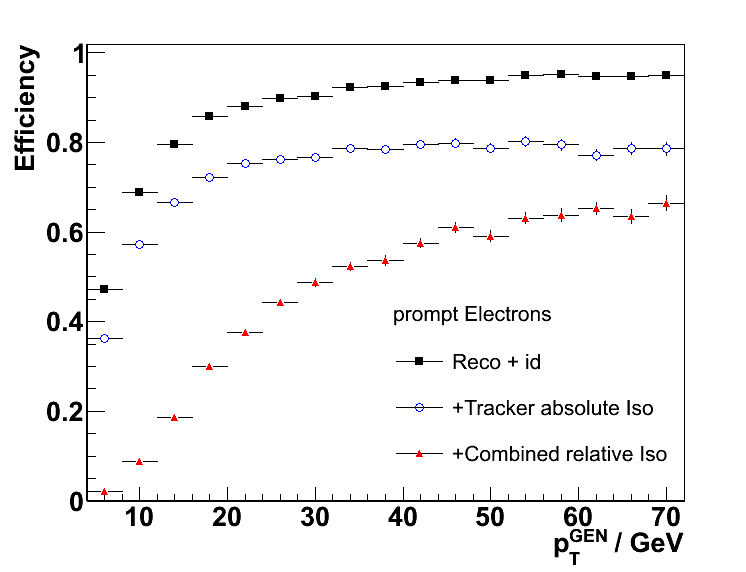
\includegraphics[scale=0.32]{./plots/prompt_ele_eff.png}}
\end{minipage}
\begin{minipage}[b]{0.5\linewidth}
\centering
{\label{fig:qcd_cor}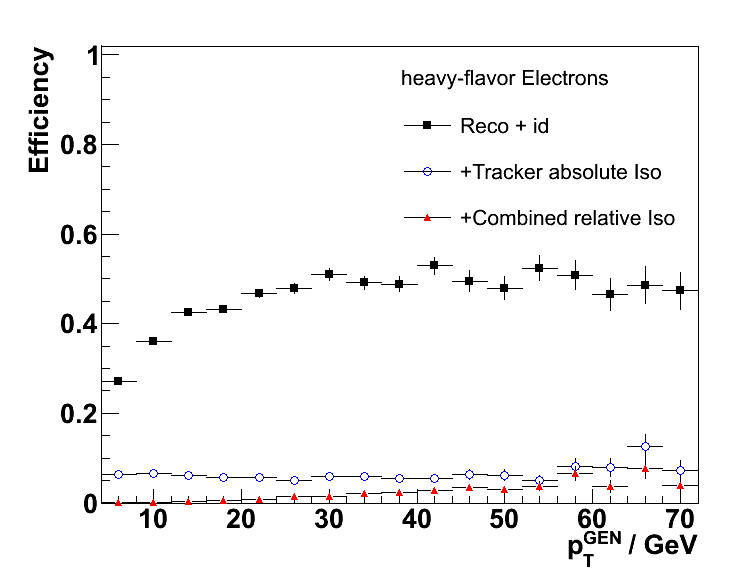
\includegraphics[scale=0.32]{./plots/hadron_ele_eff.png}}
\end{minipage}
\caption{\textit{Electron reconstruction and isolation efficiencies as a function of the generated electron $p_{T}$, for prompt electrons (left) and electrons from heavy-flavor decays (right). } }
\label{fig:ele-eff}
\end{figure}

\begin{figure}[h!]
\begin{minipage}[b]{0.5\linewidth}
\centering
{\label{fig:lm1_cor}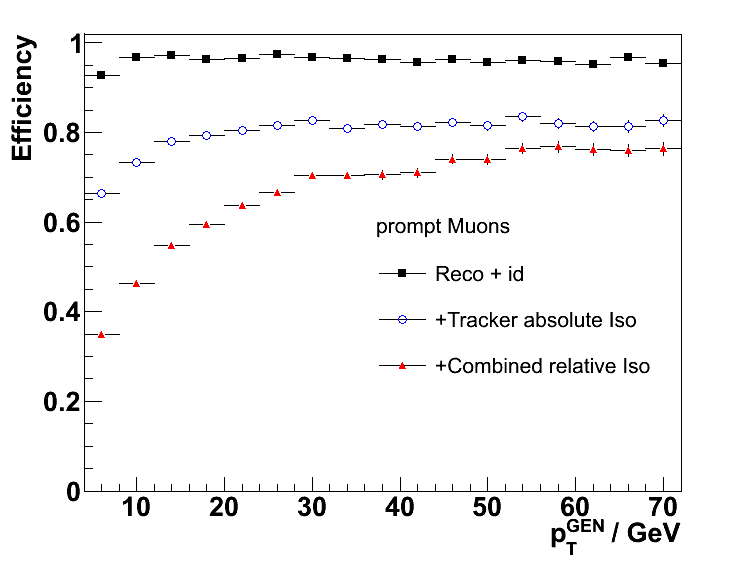
\includegraphics[scale=0.32]{./plots/prompt_muon_eff.png}}
\end{minipage}
\begin{minipage}[b]{0.5\linewidth}
\centering
{\label{fig:qcd_cor}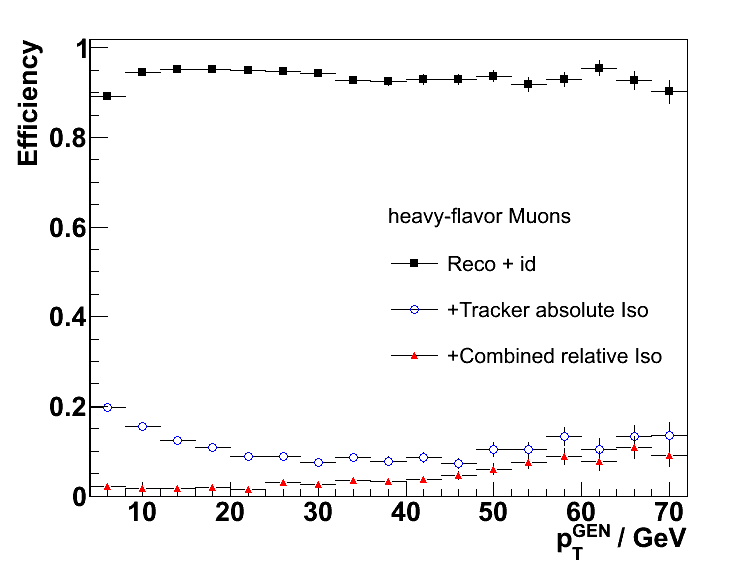
\includegraphics[scale=0.32]{./plots/hadron_muon_eff.png}}
\end{minipage}
\caption{\textit{Muon reconstruction and isolation efficiencies as a function of the generated muon $p_{T}$, for prompt muons (left) and muons from heavy-flavor decays (right). } }
\label{fig:muon-eff}
\end{figure}

\subsection{Physics objects cross cleaning}

Additional ``isolation-like'' requirements are imposed to the leptons and jets of the analysis, with the objective of resolving ambiguities between overlapping objects. In general, it is quite usual in the reconstruction, that some low-level detector information (e.g. energy deposit in the calorimeters) is shared between different candidate objects. In many of the cases, this effect may result in duplication of the energy, which in turn distroits the overall energy balancing in the event. Therefore, one needs to apply an object cleaning across different collections of reconstructed candidates (electrons, muons, jets etc). 

For the current analysis, it is vital to apply an electron-jet cleaning, so that not to count an isolated electron as an additional (fake) jet which appears in the jet collection. Furthermore, a muon-jet cross-cleaning is necessary to correct for the energy in jets taken by a (non-isolated) muon, in the heavy-flavor decays. The overall cleaning requirements are based on whether the electron or muon is isolated or not. In short, the following cross-cleaning steps have been applied: \\

\noindent \textbf{Electron-jet cross cleaning}: for each electron passing the ID criteria, the shared energy between the electron and its closest jet (within $\Delta R = 0.5$) is calculated, based on the electronmagnetic energy in towers shared by the two objects. If the electron is isolated, the shared energy is subtracted from the jet, and both objects are kept in the event. If, however, the ratio of shared energy to electron energy is above a threshold (0.7), then the jet is completely removed. If the electron is non-isolated and the shared energy is above a threshold, then the electron is removed and its energy minus the shared energy added vectorially to the jet. All other electrons, not passing the ID requirements and having an overlap with a jet, are rejected from the event.

\noindent \textbf{Muon-jet cross cleaning}: only muons passing the quality and identification criteria are considered. If the muon is not isolated and within a $\Delta R < 0.5$ from a jet, then the muon is dropped and its energy is added vectorially to the jet.

Other cross-cleaning procedures between different combinations of collections are applied such as: photon-jet cross-cleaning, with similar considerations as in the electron-jet case, as well as electron-photon cross-cleaning in order to remove fake photons originating from electrons.

\begin{comment}

\nonindent \textbf{Electron-jet cross cleaning}: if an isolated electron is found close to a jet (with EMF$<0.9$), i.e. $\Delta R (\textrm{e-Jet}) < 0.5$, and within a cone of 0.5, then the event is considered to be ambiguous and it is vetoed. If there is a non-isolated electron found in the event, then this is rejected if it has $p_{T} < 30$~GeV\footnote{In general, a non-isolated electron is most likely a fake electron, originating from a jet. For low $p_{T}$ non-isolated electrons, the source jet is also on average of low $p_{T}$ which may have been rejected by the jet energy threshold requirement.}. In all other cases ($p_{T}^{e} > 30$~GeV), the electron is rejected if it is found within a jet ($\Delta R(\textrm{non-iso e - Jet}) < 0.5$) - electron is included in the jet -, or otherwise, the whole event is vetoed ($\Delta R (\textrm{non-iso e - Jet}) > 0.5$).  \\

\noindent \textbf{Muon-jet cross cleaning}:

\end{comment}

%\end{itemize}


%\subsection{Event cleaning and kinematics}


%\newpage

\section{The $\alpha_{T}$ variable}

A new approach to SUSY searches, making use of the $\alpha_{T}$ variable, has been developed recently in CMS. It has been originally proposed in \cite{lisa} and was successfully applied to the all-hadronic search as a robust way of controlling the most challenging background at a hadron collider, the QCD multi-jet background. It is natural to look for extensions of this approach to the single-lepton search which maintains very significant hadronic jet and missing energy requirements which imply the presence of large backgrounds from QCD processes. This is the case especially when relatively soft leptons are included in the analysis.


\subsection{$\alpha_{T}$ in the N-jet case}
In the N-jet all-hadronic analysis \cite{njet}, the $\alpha_{T}$ variable has been redefined in such a way so as to reproduce, or ``simulate'', the kinematics of a di-jet system in a typical QCD event. The idea is to construct two ``pseudo-jets'' which balance each other in $H_{T}$, where the pseudo-jet $H_{T}$ equals the scalar sum of the transverse momenta $p_{T}$ of all the jets comprising the pseudo-jet. Jets are combined into pseudo-jets by minimizing the variable $\Delta H_{T} = | H_{T,1} - H_{T,2} |$. In this approach, the $\alpha_{T}$ variable is written as:
\bea
\alpha_{T} = \frac{1}{2} \frac{H_{T} - \Delta H_{T}}{M_{T}} =  \frac{1}{2} \frac{H_{T} - \Delta H_{T}}{\sqrt{H_{T}^{2}-MH_{T}^{2}}}
\eea

For a perfectly balanced system, we expect $\Delta H_{T} = 0$; in practice, mis-measurements of the jet energies as well as the exclusion of physics objects (in this case jets) due to acceptance or the quality cuts, cause a deviation of the $\Delta H_{T}$ variable from this (ideal) value. In this sense, $\Delta H_T$ is a measure of each kind of instrumental effect that distorts the momentum balance of the N-jet system.

An interesting feature of the $\alpha_{T}$ variable is the handling of the correlation of two quantities in a pseudo-dijet system: that is the correlation of the $\Delta H_T / H_T$ with the $MH_T / H_T$ variable. In an event topology with real sources of missing Energy (MET), a possible imbalance of a di-jet (or a pseudo-dijet) system is reflected in $\Delta H_T$, but also in MHT. The former will reflect an imbalance of the scalar energies, while the latter will show the angular deviation from a perfectly balanced system. It is understood that the deviation of $\Delta H_T$ is reflected in a deviation in the $MH_T$.
The relation between these two quantities is expected to show a strong correlation in a di-jet system, unless there is some source of real missing $H_T$ (that is MH$_T$ or MET). We therefore expect that a QCD di-jet system should display a correlation between these two variables. In the SUSY signal topology, on the other hand, where the presence of the two LSPs cause significant (real) MHT, this correlation should be much weaker.

\subsection{$\alpha_{T}$ in the N-jet plus 1-lepton case}

In the single-lepton analysis, the final state signature comprises one lepton in addition to the N-jet objects with respect to the all-hadronic analysis. The formation of the $\alpha_{T}$ variable implies in the same way, the requirement of at least two high-$p_{T}$ jets which are used to construct the pseudo-dijet system.
 The sources of the one lepton object in the 1-lepton final state are, whatsoever, similar to those producing a jet (quark) in the 0-lepton final state for jet multiplicities $N_{\textrm{jets}} \geq 3$. Such sources involve, namely, the charginos/neutralinos as well as the vector-bosons W and Z's decaying either hadronically (0-lepton mode) or leptonically (1-lepton mode).

Therefore, typical events of the 0-lepton and 1-lepton SUSY mode searches, appear generically similar but fall into different categories due to the presence (or absence) of a lepton, e.g.: 
\bea
 pp \rightarrow \tilde{q}_{R} \tilde{q}_{L} \rightarrow
 \begin{cases}
  q \tilde{\chi}_{1}^{o} \\ q \tilde{\chi}_{1}^{\pm} \rightarrow
\begin{cases}  q q \bar{q}' \tilde{\chi}_{1}^{o} \;\;\; \textrm{in \bf{0-lepton mode}} \\
 q \ell^{\pm} \tilde{\nu}_{\ell} \tilde{\chi}_{1}^{o} \;\;\; \textrm{in \bf{1-lepton mode}} \end{cases} \end{cases}
\eea

Having said that, the single-lepton analysis extends the definitions of the kinematic variables $\Delta H_{T}$, $MH_{T}$, $H_{T}$ and eventually $\alpha_{T}$, to include the lepton object in addition to jets. There exists, however, a correlation between the shape of these kinematic variables with the object multiplicity. A strong correlation appears in the $\Delta H_{T}$ and $MH_{T}$ variables which can be seen in fig.~\ref{fig:obj-mult} for different jet-multiplicities in the 0-lepton mode. The figures show that the values of these variables decrease on average with increasing the object multiplicity\footnote{The reason is that the higher the object multiplicity the more combinations can be formed to minimise the $\Delta H_{T}$ for example.}. It is therefore natural to assign an association between the N-jet bin of the 0-lepton analysis and the (N-1)-jet plus 1-lepton bin of the 1-lepton analysis. Kinematic variables, like the $\alpha_{T}$, will then resemble in shape between the 0-lepton and 1-lepton final states when compared in the same ``object'' multiplicity bin\footnote{A small discrpancy is however expected due to the different jet and lepton $p_{T}$ thresholds as well as the presence of an extra neutrino in the 1-lepton final state.}. Figure \ref{fig:kin} illustrates this effect for the $\alpha_{T}$ and $MH_{T}$ variables, in three object-multiplicity bins ($N_{\textrm{obs}}=3,4,5$).

\begin{figure}[h!]
\begin{minipage}[b]{0.5\linewidth}
\centering
{\label{fig:lm1_cor}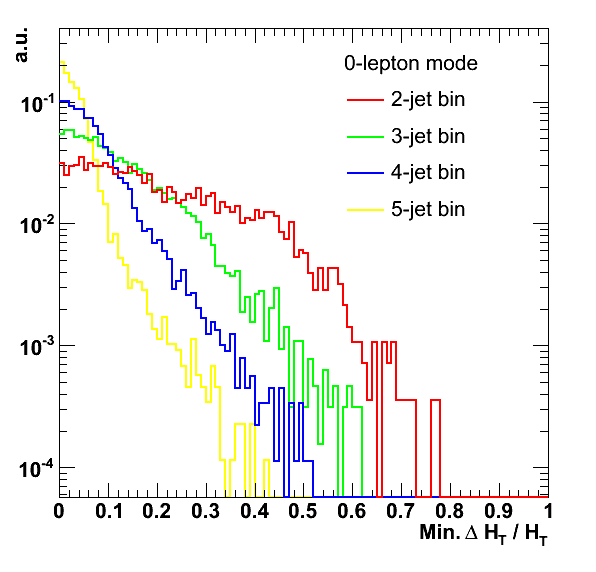
\includegraphics[scale=0.36]{./plots/dht_njet.png}}
\end{minipage}
\begin{minipage}[b]{0.5\linewidth}
\centering
{\label{fig:qcd_cor}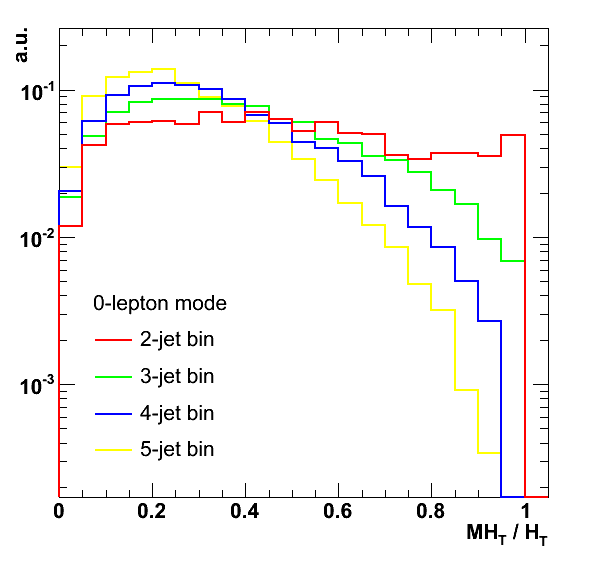
\includegraphics[scale=0.36]{./plots/mht_njet.png}}
\end{minipage}
\caption{\textit{The $\Delta H_{T}$ (left) and $MH_{T}$ (right) distribution at LM0, decomposed in N jet-multiplicity bins (N = 2, 3, 4, 5), for the all-hadronic channel.} }
\label{fig:obj-mult}
\end{figure}

\begin{figure}[h!]
\begin{minipage}[b]{0.5\linewidth}
\centering
{\label{fig:lm1_cor}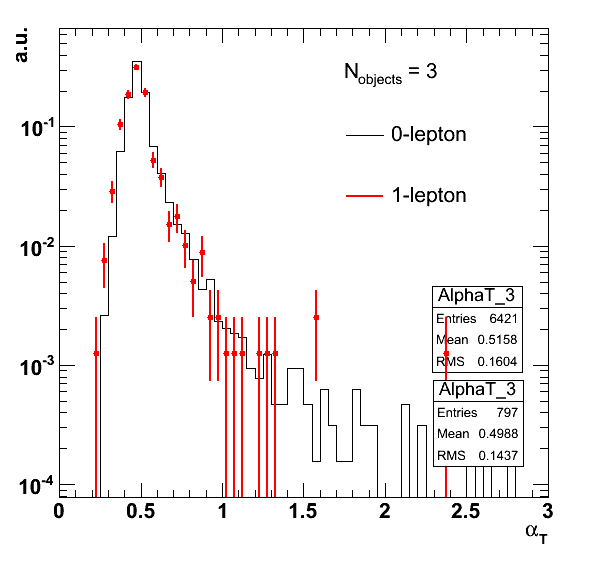
\includegraphics[scale=0.36]{./plots/aT_njet.png}}
\end{minipage}
\begin{minipage}[b]{0.5\linewidth}
\centering
{\label{fig:qcd_cor}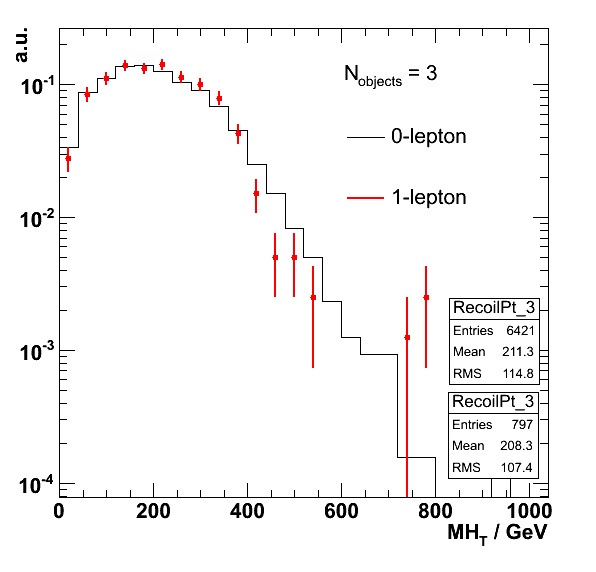
\includegraphics[scale=0.36]{./plots/recoil_njet.png}}
\end{minipage}
\caption{\textit{The $\alpha_{T}$ (left) and $MH_{T}$ (right) shapes at LM0, decomposed in object-multiplicity bins (N = 3, 4, 5 objects), for the all-hadronic and 1-lepton mode SUSY channels superimposed. }}
%The agreement in shape is obvious between the two channels, for the same object multiplicity - $N_{0-lepton}$ = n-jets and $N_{1-lepton}$=(n-1)-jet + 1-lepton.} }
\label{fig:kin}
\end{figure}


\begin{comment}
\begin{figure}[h!]
\begin{minipage}[b]{0.5\linewidth}
\centering
{\label{fig:lm1_cor}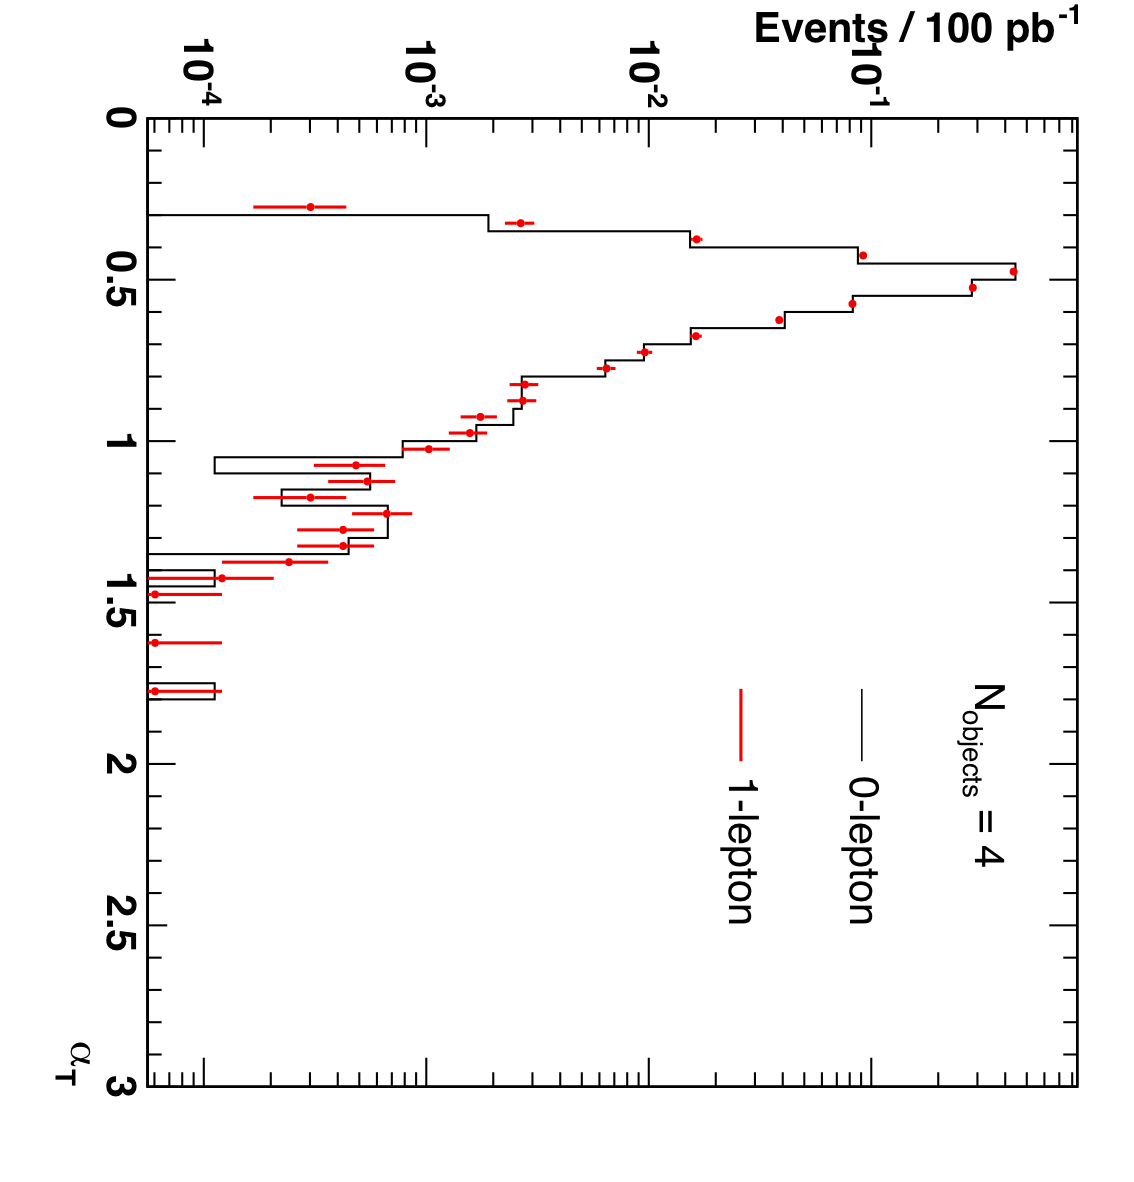
\includegraphics[scale=0.36, angle=90]{./plots/aT_4}}
\end{minipage}
\begin{minipage}[b]{0.5\linewidth}
\centering
{\label{fig:qcd_cor}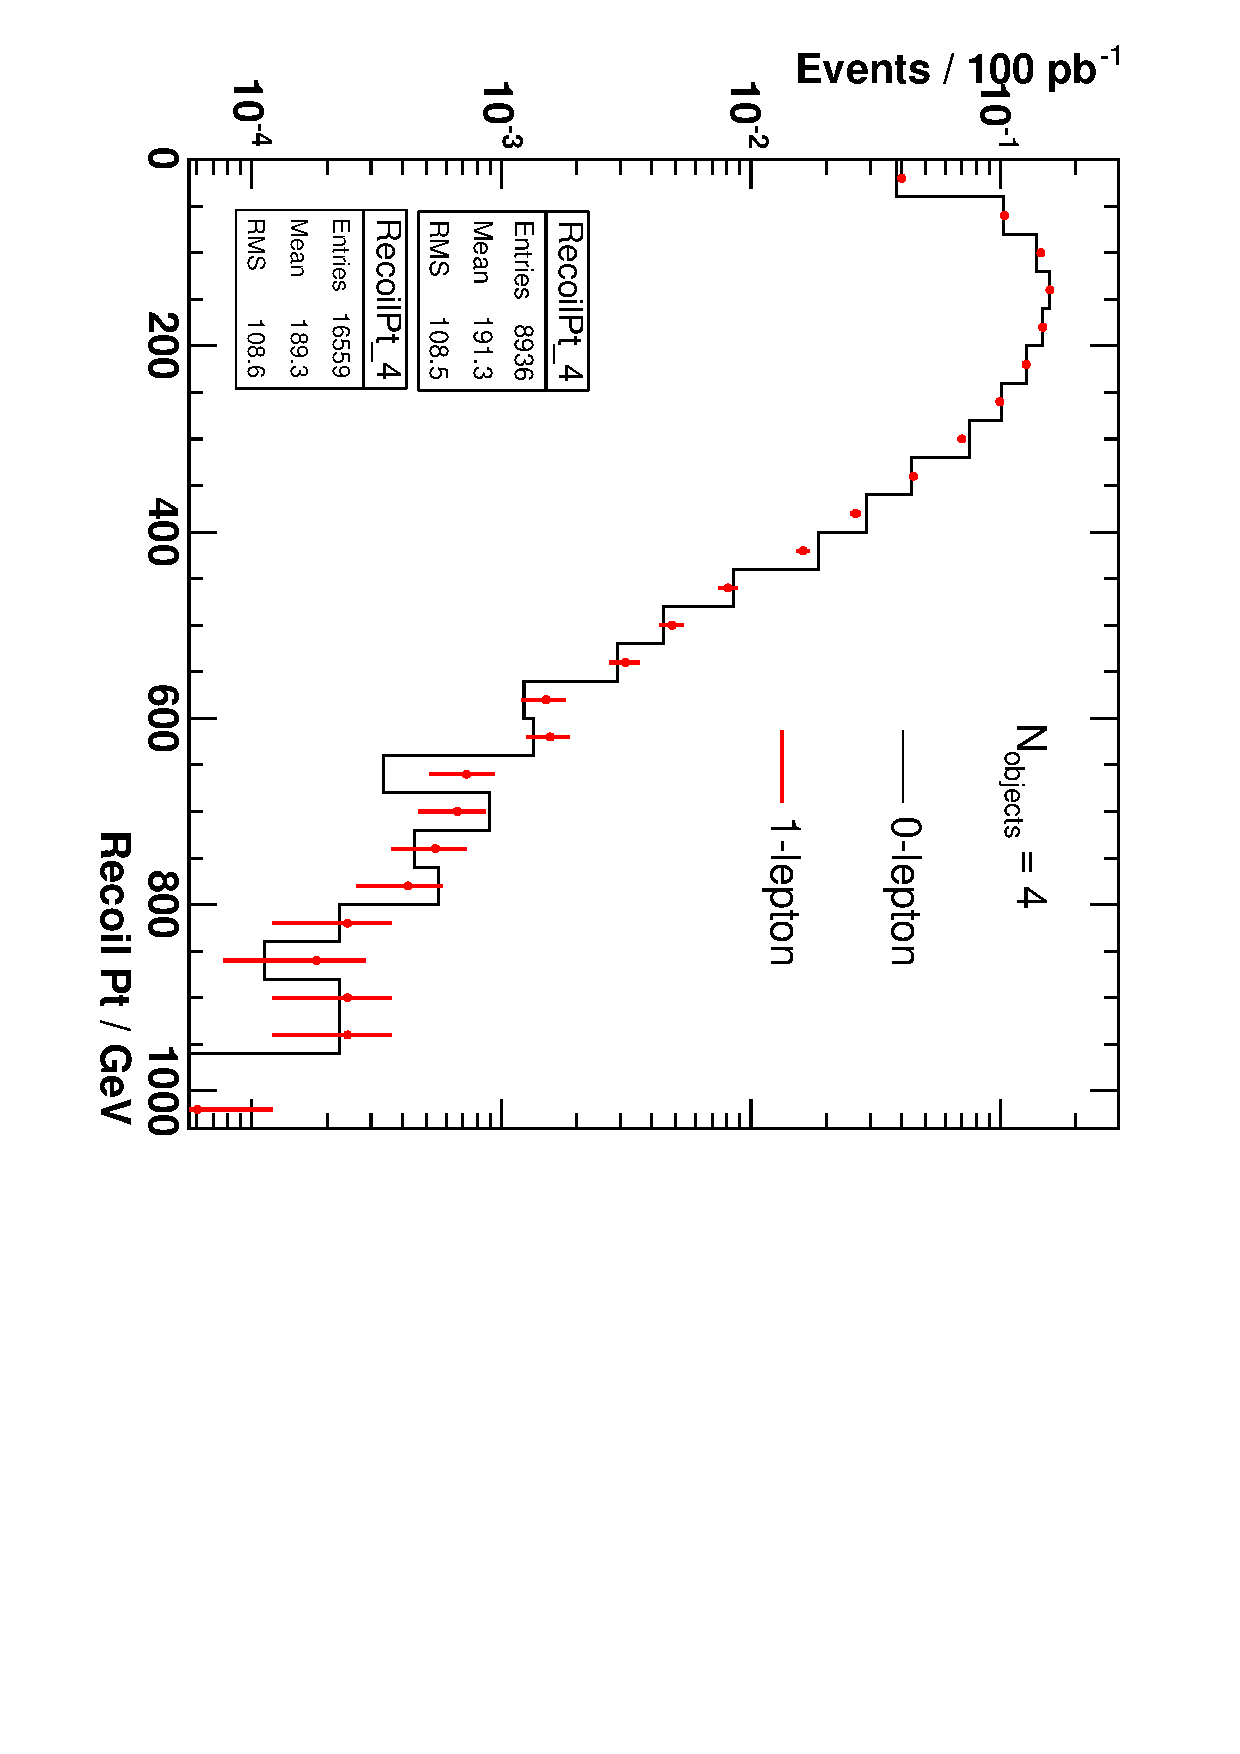
\includegraphics[scale=0.36, angle=90]{./plots/mht_4}}
\end{minipage}
%\caption{\textit{} }
\label{fig:cor}
\end{figure}
\begin{figure}[h!]
\begin{minipage}[b]{0.5\linewidth}
\centering
{\label{fig:lm1_cor}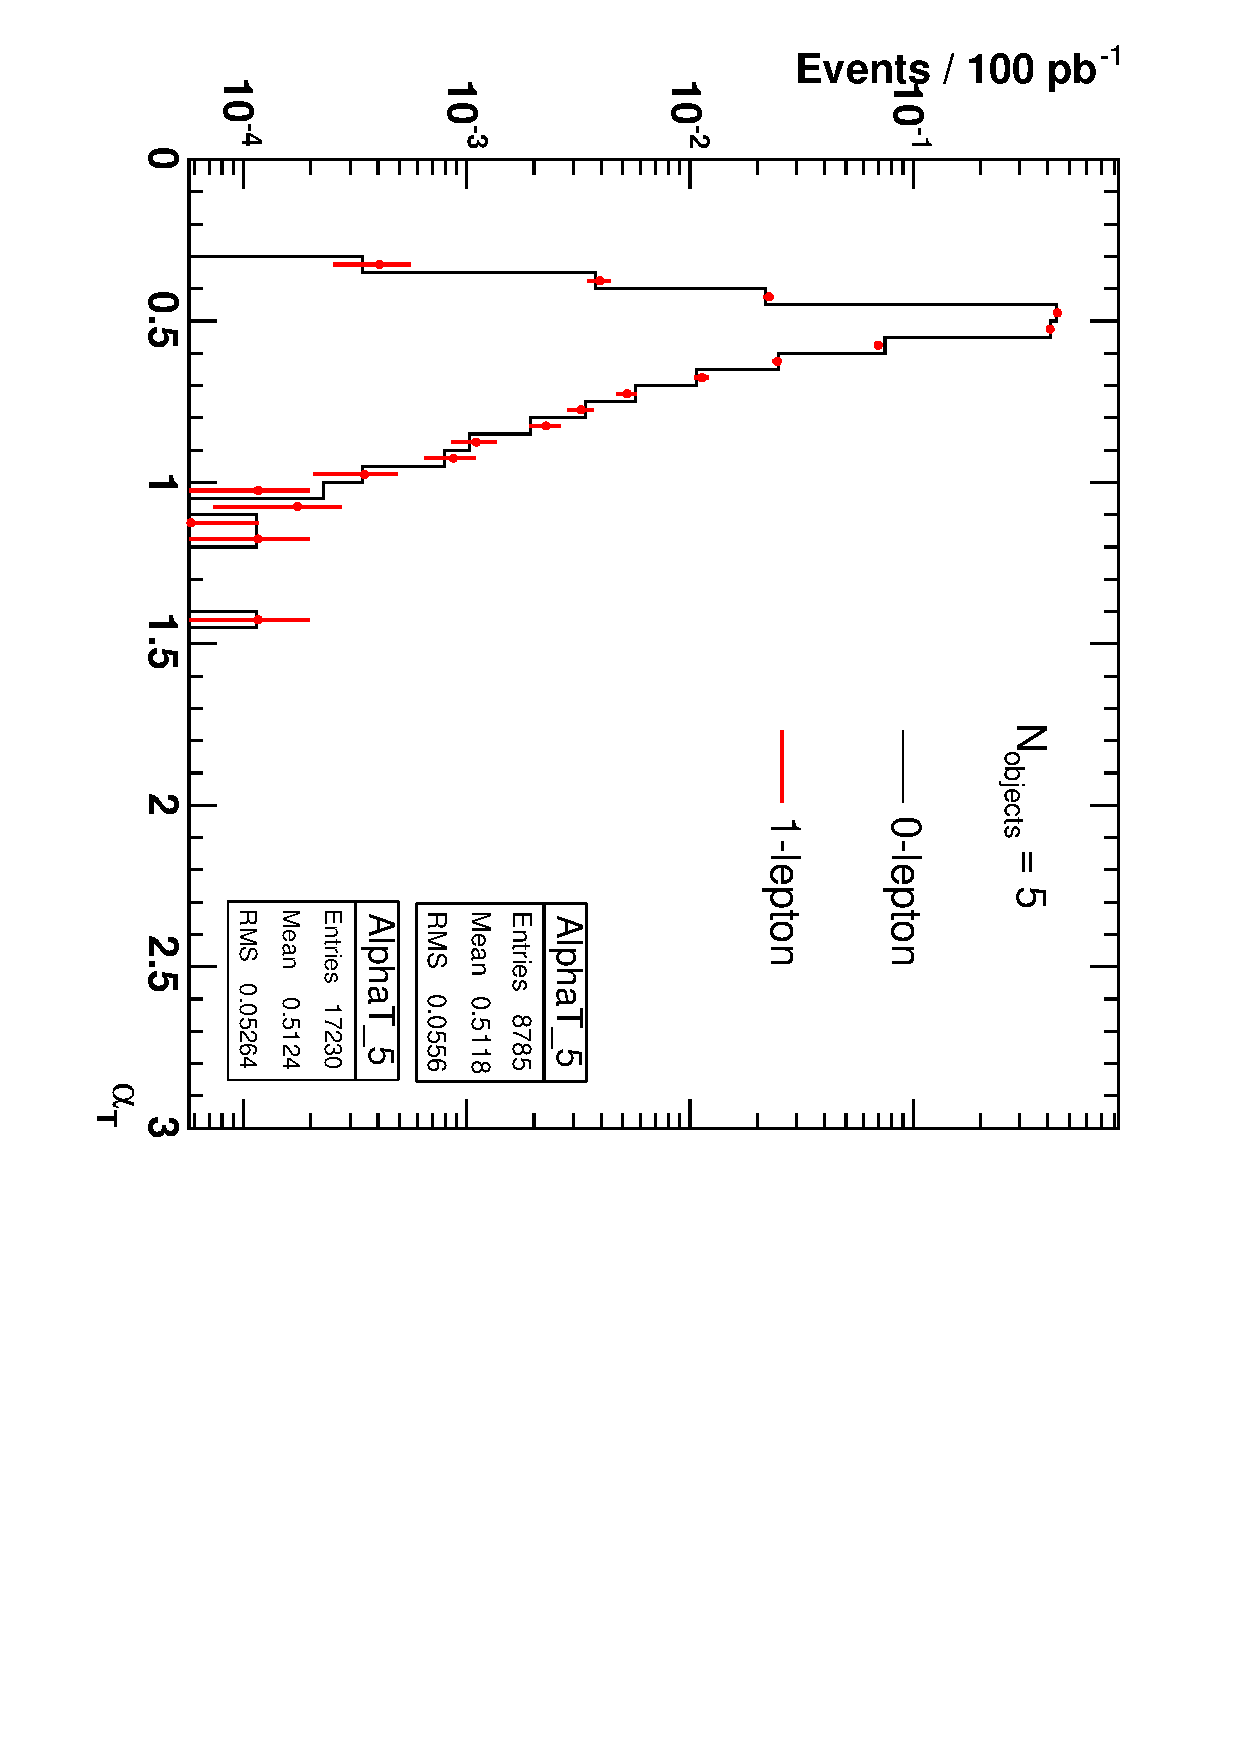
\includegraphics[scale=0.36, angle=90]{./plots/aT_5}}
\end{minipage}
\begin{minipage}[b]{0.5\linewidth}
\centering
{\label{fig:qcd_cor}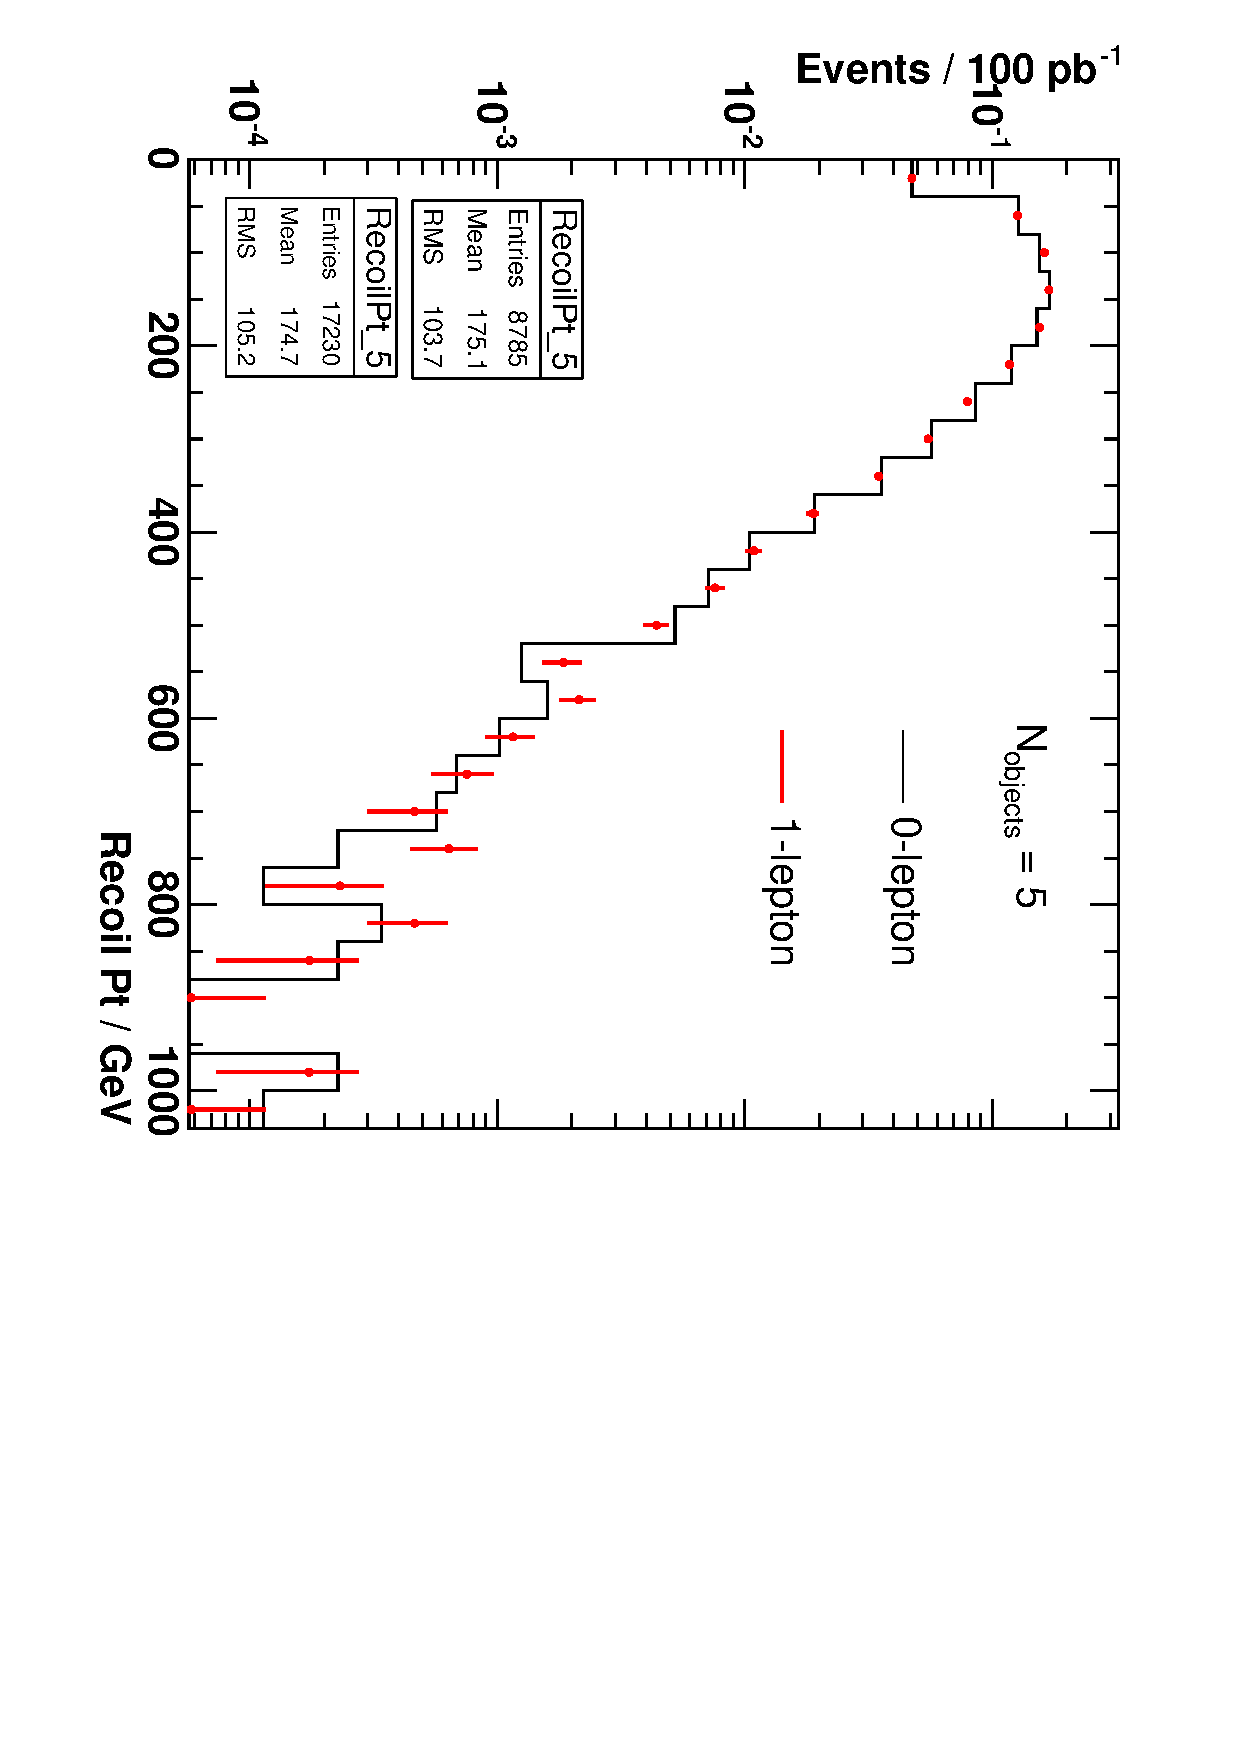
\includegraphics[scale=0.36, angle=90]{./plots/mht_5}}
\end{minipage}
\caption{\textit{\small {The $\alpha_{T}$ (left) and $MH_{T}$ (right) shapes at LM0, decomposed in object-multiplicity bins (N = 3, 4, 5 objects), for the all-hadronic and 1-lepton mode SUSY channels superimposed. The agreement in shape is obvious between the two channels, for the same object multiplicity - $N_{0-lepton}$ = n-jets and $N_{1-lepton}$=(n-1)-jet + 1-lepton.}} }
\label{fig:kin}
\end{figure}
\end{comment}

The ``leptonic'' version of the $\alpha_{T}$ variable is intended to control the QCD background which survives the one-lepton selection due to fake leptons or leptons from heavy-flavor decays. It has been shown to maintain the good performance in controling the QCD background as in the all-hadronic channel. This is illustrated in fig.~\ref{fig:cor}, which shows the correlation between the $\Delta H_{T}$ and $MH_{T}$ in the one-lepton channel, for the SUSY signal and the QCD N-jet background. One can notice that in the case of QCD (right plot), the correlation grows strong across the diagonal where the severe mismeasurements appear: large values of $\Delta H_{T}$ are grown along with large values of $MH_{T}$.

The functional form of the (leptonic) $\alpha_{T}$ is shown on the same figure for constant values equal to 0.55. It can be seen that the curve $\alpha_{T}>0.55$ is able to reject all of the QCD events, as expected.


\begin{figure}[h!]
\begin{minipage}[b]{0.5\linewidth}
\centering
{\label{fig:lm1_cor}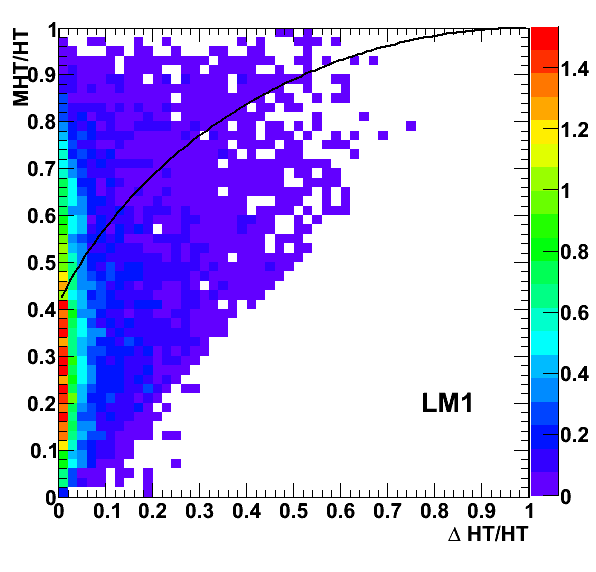
\includegraphics[scale=0.36]{./plots/lm1_cor.png}}
\end{minipage}
\hspace{3mm}
\begin{minipage}[b]{0.5\linewidth}
\centering
{\label{fig:qcd_cor}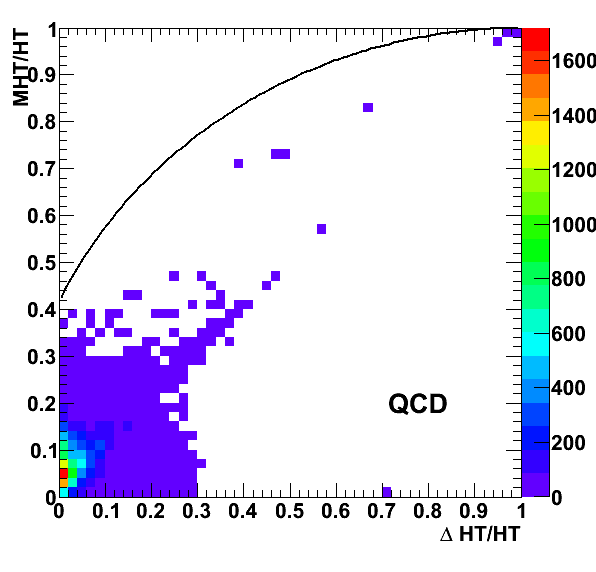
\includegraphics[scale=0.36]{./plots/qcd_cor.png}}
\end{minipage}
%\subfloat[LM1 events.]{\label{fig:lm1_cor}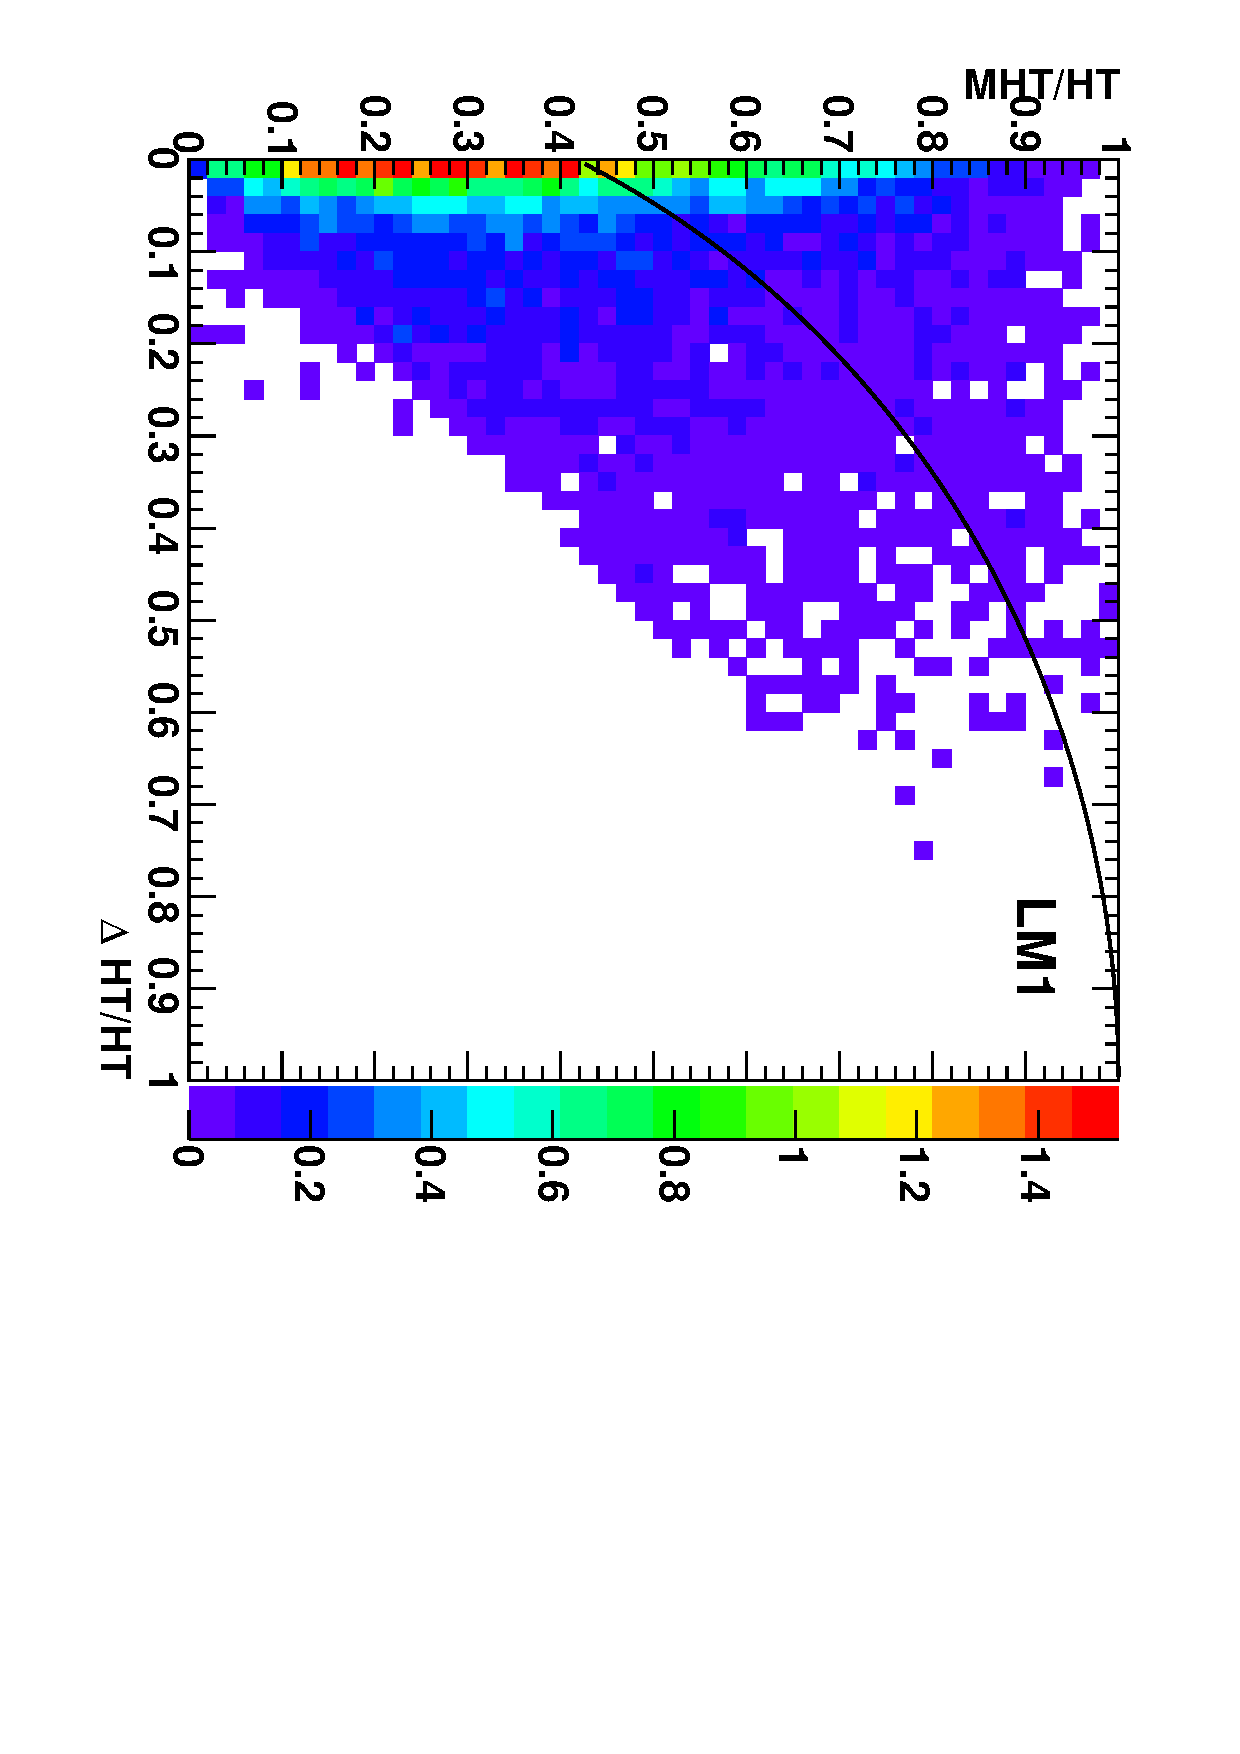
\includegraphics[scale=0.4, angle=90]{./plots/lm1_correlation_1lepton_afterHT}} 
%\subfloat[QCD plus $b\bar{b} + \textrm{jets}$ events.]{\label{fig:qcd_cor}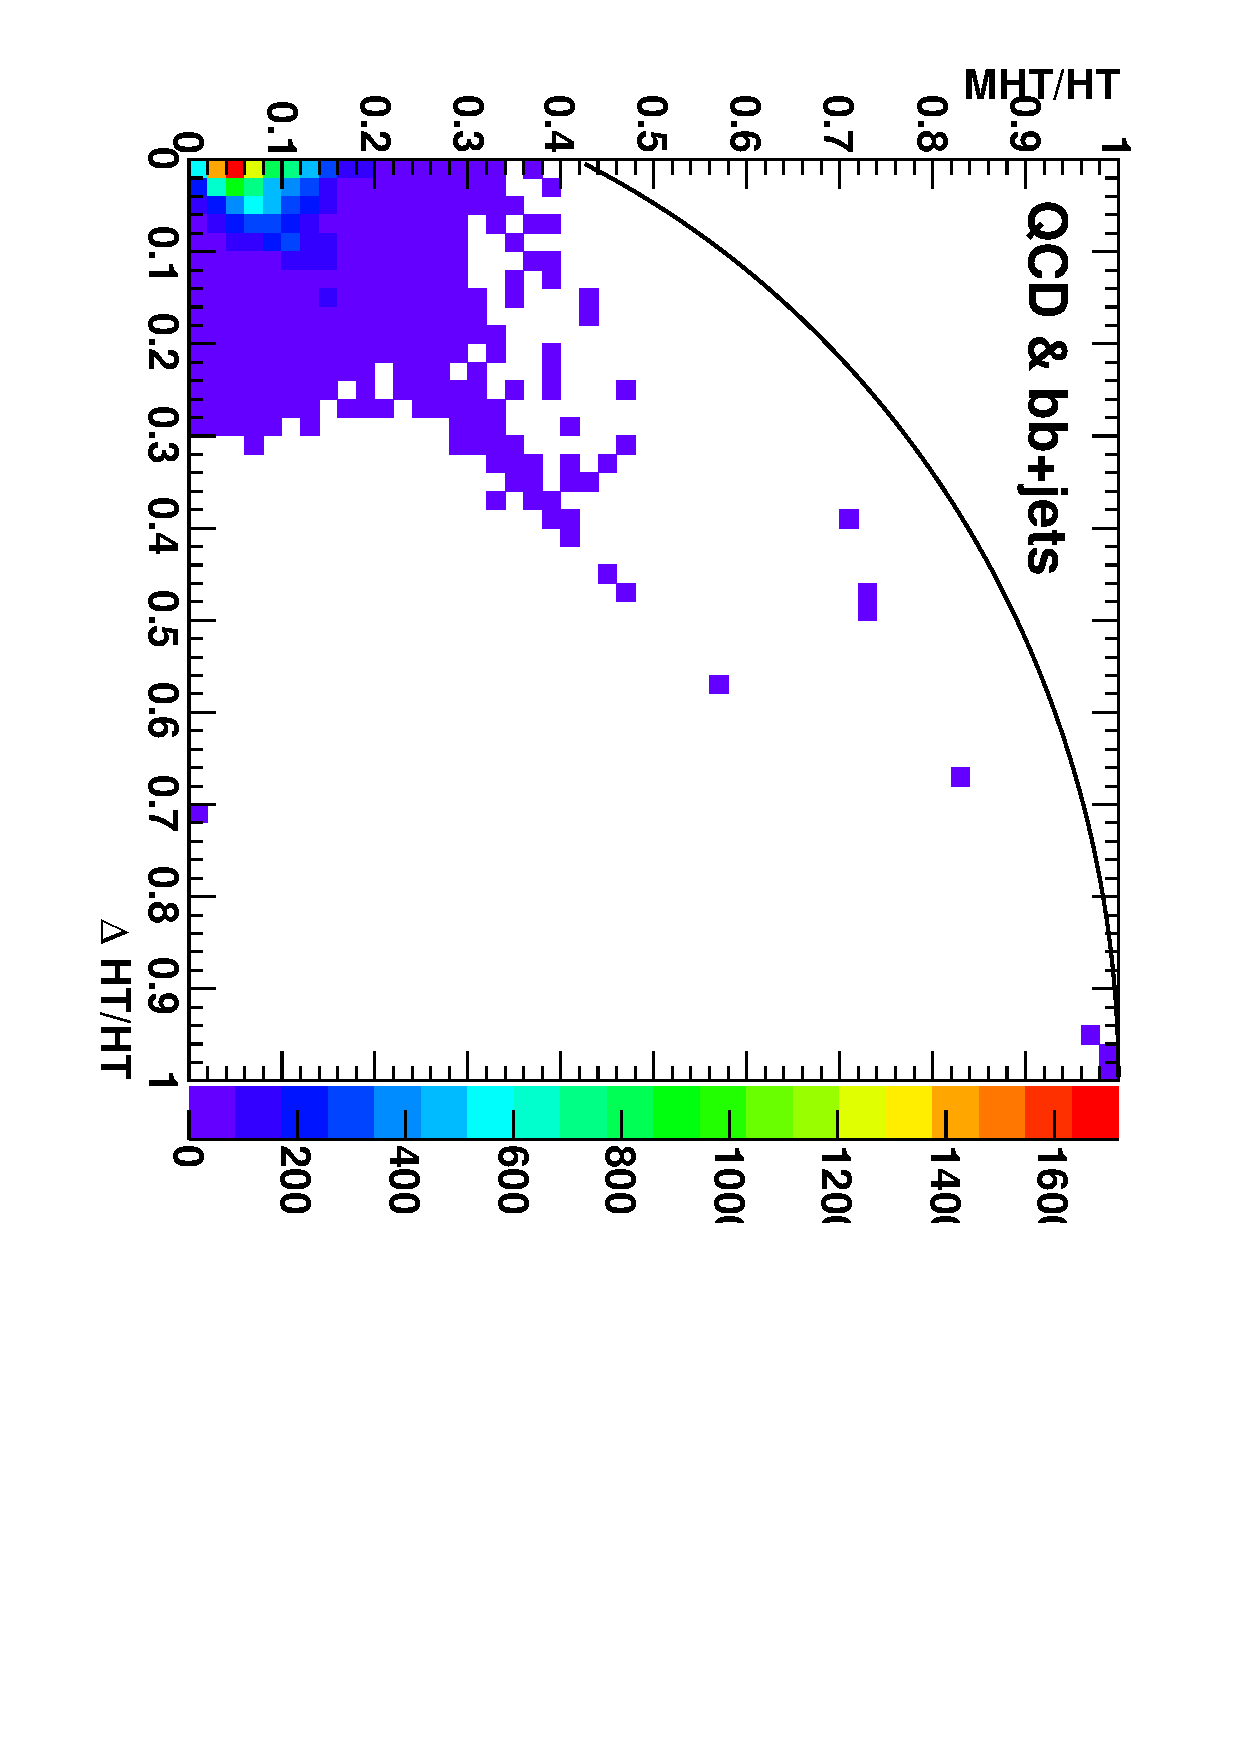
\includegraphics[scale=0.4, angle=90]{./plots/qcd_correlation_1lepton_afterHT}} 
\caption{\textit{The correlation of $\Delta H_{T}/H_{T}$ with $MH_{T}/H_{T}$ in SUSY LM1 events (a) and QCD events (b), in the 1-lepton mode channel. An $H_{T}$ cut of 350 GeV has been applied. The black line indicates constant values of $\alpha_{T}=0.55$.} }
\vspace{5mm}
\label{fig:cor}
\end{figure}

%\clearpage

\section{Analysis method and results}

\subsection{$\alpha_{T}$ selection}

The single-lepton analysis cut-flow starts with the requirement of exactly one ``good'' lepton (electron or muon), with $p_{T} > 5$ GeV, in the event. The jet cuts has been driven by the all-hadronic N-jet analysis and constist in the requirement of at least two jets with $p_{T}>30 \textrm{GeV}$ and $|\eta|<3$. The second jet must have $p_{T}>100 \textrm{GeV}$. An $H_{T}$ cut at 350 GeV is applied in addition, in order to select events with significant amount of hadronic-jet activity relevant to the SUSY environment. The final step in the selection consists of the requirement that the variable $\alpha_{T}$ should be above $0.55$. This cut is expected to supress (almost) all of the QCD N-jets (including $b\bar{b} + \textrm{jets}$) events, as explained earlier.

Figures ~\ref{fig:dists1} and ~\ref{fig:dists2} display the distributions of basic kinematic observables that are utilized in the analysis, for all the SM backgrounds and the SUSY signal (LM0 and LM1), after the standard selection but the $\alpha_{T}$ cut. Such observables, besides the $\alpha_{T}$ itself, are basically the recoil missing transverse energy, $MH_{T}$, defined as the vectorial sum of the energies of all jets plus the lepton in the event:
\begin{eqnarray}
MH_{T}= - \sum_{i = 1,..,N} p_{T}^{i , \textrm{jet}} + p_{T}^{\ell}
\end{eqnarray} 
and the scalar sum of the energies of all jets plus the lepton, $H_{T}$. All of these observables provide a discriminating power of the SUSY signal over the SM expectations, to some extent. As will be proven in the next sections, the $\alpha_{T}$ variable is the dominant cutting variable in terms of robustness and control over QCD jet mismeasurements.

\begin{figure}[h!]
\begin{minipage}[b]{0.5\linewidth}
\centering
{\label{fig:aT}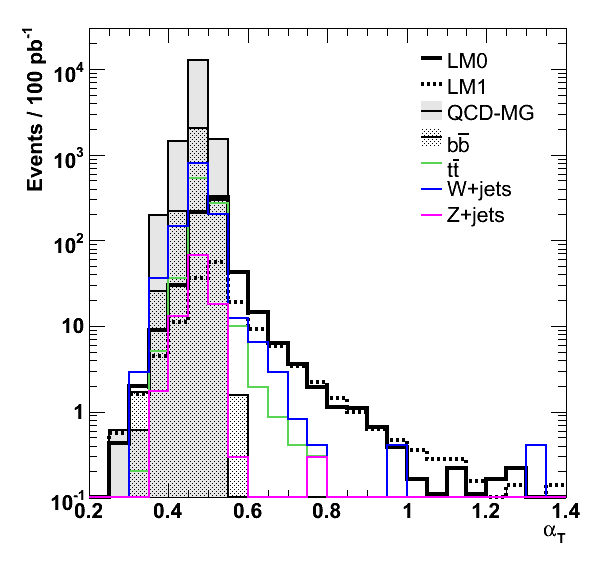
\includegraphics[scale=0.38]{./plots/aT-AllSignals.png}} 
\end{minipage}
\begin{minipage}[b]{0.5\linewidth}
\centering
{\label{fig:mht}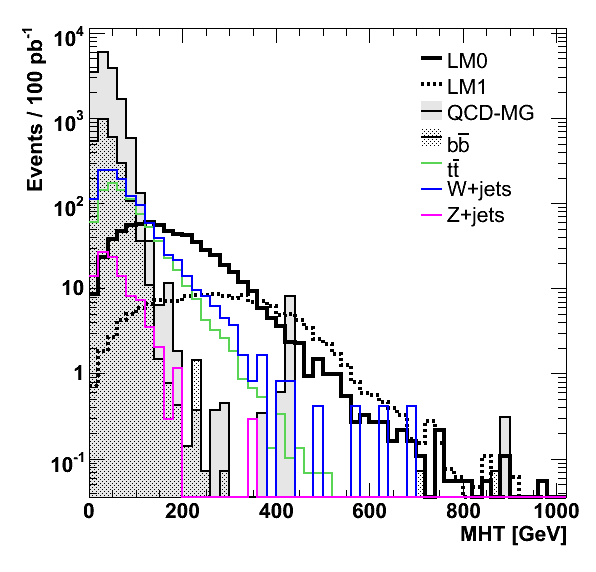
\includegraphics[scale=0.38]{./plots/MHT-AllSignals.png}} 
\end{minipage}
%\subfigure[The $\alpha_{T}$ distribution after all cuts but $\alpha_{T}$.]{\label{fig:aT}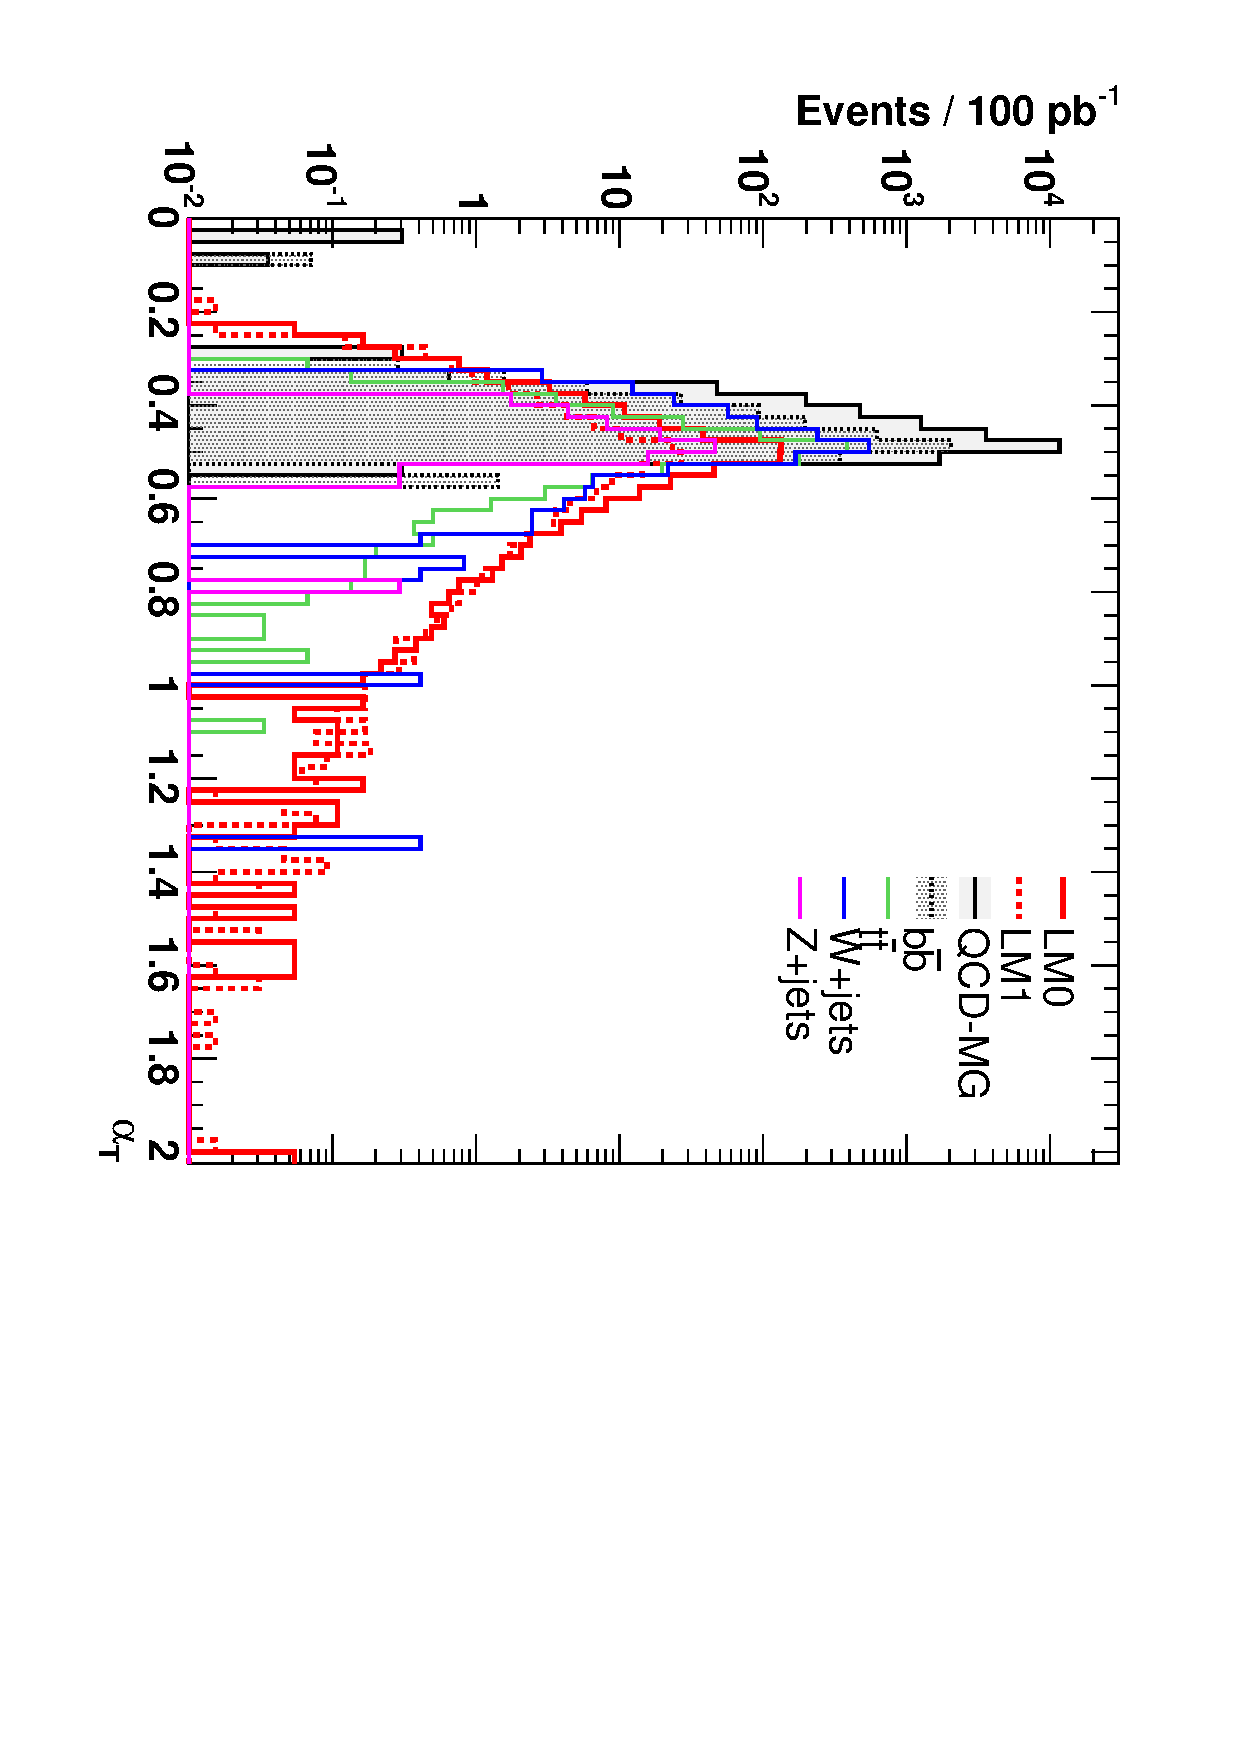
\includegraphics[scale=0.4, angle=90]{./plots/aT-NT7-SigAndBkg-AfterHTcut}} 
%\subfigure[The $\textrm{MH}_{\textrm{T}}$ distribution after all cuts but $\alpha_{T}$.]{\label{fig:mht}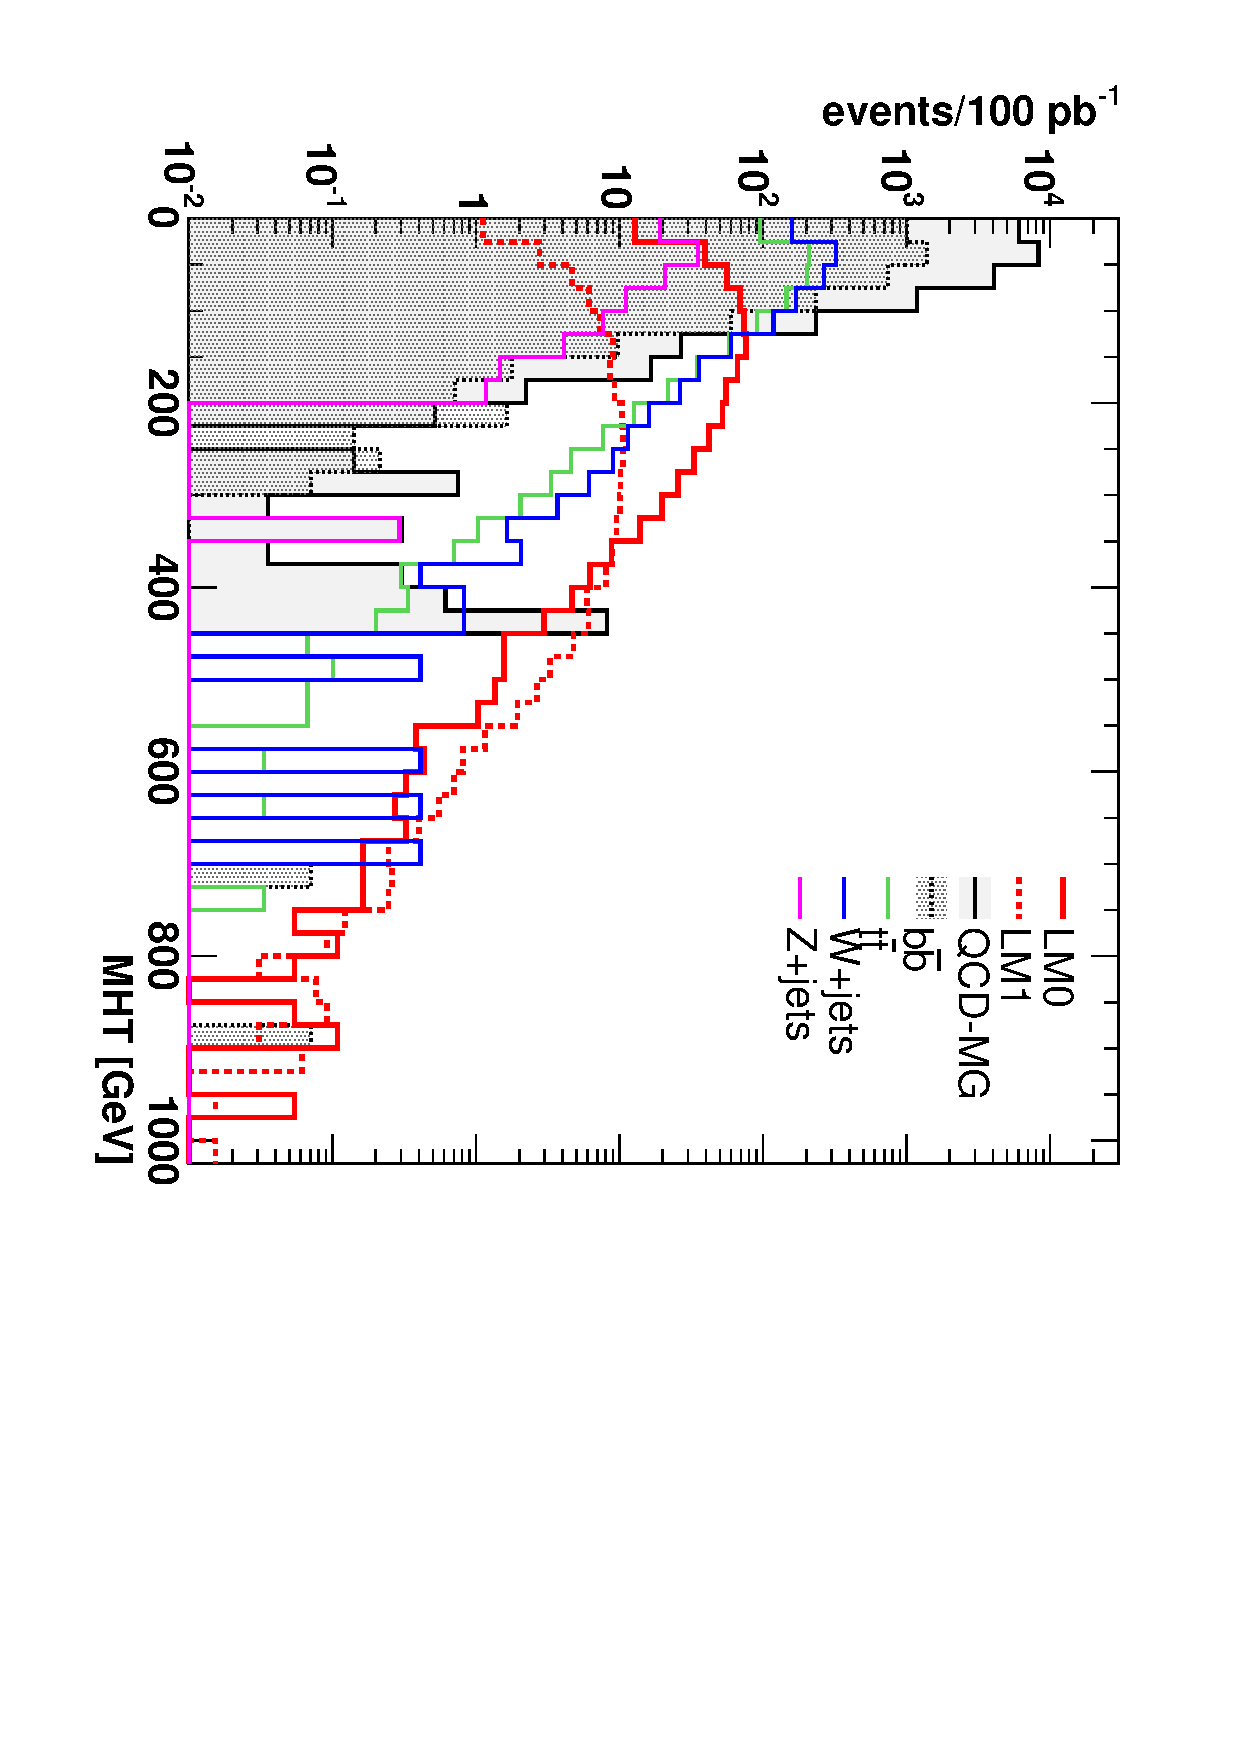
\includegraphics[scale=0.4,angle=90]{./plots/MHT-NT7-SigAndBkg-AfterHTcut}} 
\caption{\textit{The $\alpha_{T}$ (a) and $MH_{T}$ (b) distributions for the LM0 and LM1 SUSY signal and all the SM backgrounds superimposed, for an integrated luminosity of $100 \textrm{pb}^{-1}$.} }
\label{fig:dists1}
\end{figure}
\begin{figure}[h!]
\begin{minipage}[b]{0.5\linewidth}
\centering
{\label{fig:mhtovht}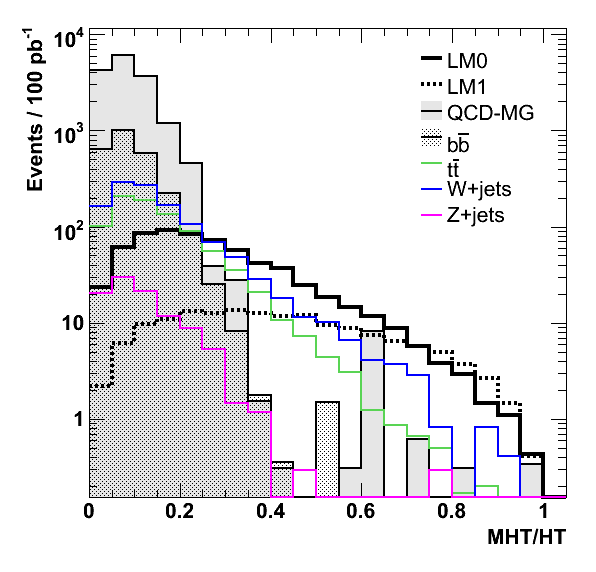
\includegraphics[scale=0.38]{./plots/MHTovHT-AllSignals.png}} 
\end{minipage}
\begin{minipage}[b]{0.5\linewidth}
\centering
{\label{fig:ht}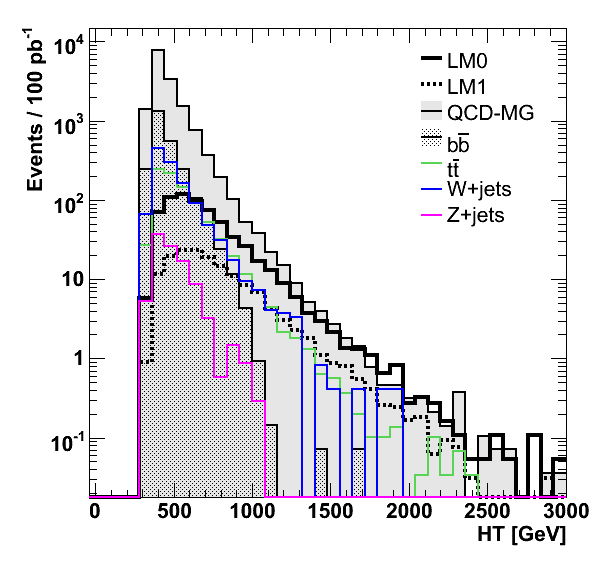
\includegraphics[scale=0.38]{./plots/HT-AllSignals.png}} 
\end{minipage}
\caption{\textit{The $MH_{T}/H_{T}$ (a) and $H_{T}$ (b) distributions for the LM0 and LM1 SUSY signal and all the SM backgrounds superimposed, for an integrated luminosity of $100 \textrm{pb}^{-1}$.} }
\vspace{5mm}
\label{fig:dists2}
\end{figure}


\subsection{Comparison with RA4}

For the sake of completeness, a comparison of the event yields between the $\alpha_{T}$ cut-flow and the RA4 selection, normalized for $100 \textrm{pb}^{-1}$ of integrated luminosity, is presented next.

The RA4 selection follows a more traditional cut-flow involving a cut in the missing transverse energy. From Monte Carlo (MC) studies, it has been shown that the missing energy variable provides a fairly good separation between the SUSY signal events, in R-parity conserving models, and most of the SM background processes ($W/Z + \textrm{jets}, t\bar{t} + \textrm{jets}$ and QCD ). Although, originally the MET cut in RA4 is rather loose (set to $100$ GeV)\footnote{A loose cut in the missing energy at $100$ GeV has been set to RA4, as the most suitable cut for the LM0 events separation, but also to allow a significant event yield in order to allow further cuts for background estimation purposes (ABCD method etc).}, we alternatively try to tighten the cut at $180$ GeV, which seems to be an optimal cut value for most of the LMx SUSY points, for the purpose of comparison with the $\alpha_{T}$ approach.

The event pre-selection for the two analysis paths ($\alpha_{T}$ versus RA4), show rather different in the two approaches:
\begin{description}
\item[$a_{T}$ approach:] i) Exactly one muon or one electron with $p_{T}>5$ GeV, while vetoing a second different-flavor lepton. Both electron and muon objects are required to satisfy the customly proposed isolation. ii) Veto on events with: a second lepton not passing the quality as well as isolation criteria or a jet outside the eta acceptance. iii) At least two jets with $p_{T}>30$ GeV, and the second leading jet $p_{T} > 100$ GeV. iv) An $H_{T} > 350$ GeV. 
\item[RA4 approach:] i) Exactly one muon or one electron with $p_{T}>10$ GeV, while vetoing a second different-flavor lepton. The isolation imposed on the electron and muon objects is taken from the standard V+jets recommendation (relative combined isolation). ii) At least three jets with $p_{T}>30$ GeV, and the third leading jet $p_{T}>50$ GeV. 
\end{description}

The number of events expected for $100 \textrm{pb}^{-1}$ of integrated luminosity, is calculated at each step in the cut flow, for all the SM backgrounds and the LM0 and LM1 SUSY signals. Tables ~\ref{tab:ey1} and ~\ref{tab:ey2} show the event yield in the 1-muon channel, for the $\alpha_{T}$ and RA4 approaches respectively, whereas tables ~\ref{tab:ey3} and ~\ref{tab:ey4} show the 1-electron channel numbers similarly. The $\alpha_{T}$ cut-flow includes alternatively the event-yield out of a cut on the $MH_{T}/H_{T}$ variable, which shows equivalent performance with the $\alpha_{T}$ cutting variable. The final event yield is compared between the two approaches in terms of Signal-to-Background ratio (S/B) and the signal significance ($S/\sqrt{B}$). The LM0 and LM1 points were used as the SUSY signal.

It can be seen that, the input lepton selection differs significantly between the RA4 and $\alpha_{T}$ approaches as a result of the different lepton $p_{T}$ thresholds and the isolation requirements. In both muon and electron channels, the dominant background contributions come from the W+jets and $t\bar{t}$+jets events. It is interesting to notice that in the case of the $\alpha_{T}$ (or equivalently the $MH_{T}/H_{T}$) cut-flow, the W gets higher than the $t\bar{t}$ and almost twice as that. This is opposed to the RA4 selection result where the dominant background is by far the $t\bar{t}$. The effect can be understood by the inclusion of the 2-jet bin in the $\alpha_{T}$ selection which maintains a large amount of $W$ events, opposed to RA4. Moreover, a direct cut on the $MH_{T}/H_{T}$ variable (or an indirect one using the $\alpha_{T}$), enhance in addition the W events\footnote{With the given high $H_{T}$ cut (350 GeV), $MH_{T}/H_{T}$ falls more rapidly for the $t\bar{t}$ events than the W's in the tails of such a distribution.}. For what concerns the QCD/$b\bar{b}$ backgrounds, these are drastically suppressed only after the final step in the selection ($\alpha_{T}$ or $ME_{T}$ cut). The striking result is the strong suppression of the QCD using the $\alpha_{T}$ selection, leaving zero events after a cut on $\alpha_{T}$. 

With the LM0/LM1 being the SUSY signal, the $S/B$ shows comparable performance between the $\alpha_{T}$ approach and RA4, whereas an improved significance is observed in the final signal significance when the RA4 cut-flow is used. The reduced signal event yield of the $\alpha_{T}$ approach\footnote{With an improved ``EMF treatment'' in the one-electron channel, it is possible to achieve a significance above 5 - thus significantly improving the results presented in this note. Still, since the major focus is now on the commissioning of the analysis with real data rather than continued MC studies, that was postponed for later versions of the Note.} indicates a first drawback of the method. Nevertheless, as it will be shown in the next sections, the $\alpha_{T}$ shows a strong advantage compared to RA4 when arguments of robustness against jet energy mismeasurements (mainly introduced by QCD jet events) are considered.

\begin{table}[h!]
\vspace{3mm}
   \centering
   \begin{tabular*}{0.95\textwidth}{@{\extracolsep{\fill}}| c | c c c c c c c |}
      \hline	
	Selection cut & QCD & $b\bar{b}$ & Z & W & $t\bar{t}$ & LM1 & LM0 \\ \hline
		$\mu$-selection & 2414.2 & 619. & 59095.5 & 716527. & 4502.9 &175.7 &1247.6 \\ 
3-jet cut & 649.6 & 160.9 & 106.6 & 987.9 &1639. &95.3 & 752.8 \\ \hline \hline
\small{$ME_{T}>100$} & 1.3 & 1.9 & 8.8 & 176.5 & 356.1 &85.6 & 498.3  \\ \hline 
	\small{$ME_{T}>180$}  & $7 \cdot 10^{-2}$ & 0 & 0.9 & 37.3 & 51.5 & 66.7 & 232.2  \\ \hline
\end{tabular*}
   \caption{\textit{\small{Event-yield out of the RA4 cut-flow, normalized to $100 \textrm{pb}^{-1}$, in the one-muon channel. }}}
   \label{tab:ey1}
\end{table} 

\begin{comment}

\begin{table}[h!]
\vspace{5mm}
   \centering
    \begin{tabular*}{0.95\textwidth}{@{\extracolsep{\fill}}| c | c c c c c c c |}
%   \begin{tabular}{|c|ccccccc|}
      \hline
	Selection cut & QCD & $b\bar{b}$ & Z & W & $t\bar{t}$ & LM1 & LM0  \\ \hline
		$\mu$-selection & 50860. & 14118.2 & 59862.9 & 752110. &  4822.6 & 186. & 1368.3 \\
		2-jet cut & 11364.3	 & 3031.2 & 131.8 & 1134. & 883.5 & 124. & 686.7 \\ 
		$H_{T}$ cut & 5477.9 & 1444.2 & 89.9 &  786.8 & 786.9 & 121.9 & 670.0 \\ 
			Odd cuts & 1504.4 & 405.5 &   46.6 &  568.1 & 438.4 & 69. & 335. \\ \hline \hline
		\small{$\alpha_{T}>0.55$ }& 0 & <1 & 0.3 & 11.5 & 7.0 & 20.1 & 34.3 \\ \hline
%		\scriptsize{$MH_{T}/H_{T}>0.4$} & &&&&&&&&\\ \hline
			
 \end{tabular*}
    
\caption{\textit{\small{Event-yield out of the $\alpha_{T}$ cut-flow with leptons of $p_{T}>10$ GeV, normalized to $100 \textrm{pb}^{-1}$, in the one-muon channel. }}}
   	\label{tab:ey2}
\end{table} 
\begin{table}[h!]
\vspace{5mm}
   \centering
    \begin{tabular*}{0.95\textwidth}{@{\extracolsep{\fill}}| c | c c c c c c c |}
%   \begin{tabular}{|c|ccccccc|cc|}
      \hline
	Selection cut & QCD & $b\bar{b}$ & Z & W & $t\bar{t}$ & LM1 & LM0  \\ \hline
		$\mu$-selection & 177681.6 & 34484.2 & 66107.5 & 808264. & 5233.5 & 230.1 & 1554.8 \\
			2-jet cut & 45369.9 & 8341.5 & 144.7 & 1202.2 & 991.8 & 153.3 & 789.3 \\ 
		$H_{T}$ cut & 20017.12 & 3613.6 & 94.9 & 822.9 & 880.3 & 150.6 & 768.7 \\ 
		Odd cuts & 7493.8 & 1211.3 & 47.5 & 579.9 & 451.1 & 80.5 & 359.3 \\ \hline \hline
		\small{$\alpha_{T}>0.55$ }& 0.3 & 0.07 & 0.6 & 13.5 & 7.3 & 23.7 & 39.8 \\ \hline
%		\scriptsize{$MH_{T}/H_{T}>0.4$} & 0.3 & 0.7 & 0.6 &33.2 & 15.2 & 44.1 & 76.6 & 1.5 & 10.8\\ \hline
			
 \end{tabular*}
  
\caption{\textit{\small{Event-yield out of the $\alpha_{T}$ cut-flow with leptons of $p_{T}>5$ GeV, normalized to $100 \textrm{pb}^{-1}$, in the one-muon channel. }}}
   	\label{tab:ey3}
\end{table} 

\begin{table}[h!]
\vspace{5mm}
   \centering
    \begin{tabular}{@{\extracolsep{\fill}}| c || c c c || c c c |}
    \hline
    &\multicolumn{3}{c||}{\textbf{LM0}} & \multicolumn{3}{c|}{\textbf{LM1}} \\ \cline{2-7}
    & RA4 & $\alpha_{T, 10}$ & $\alpha_{T, 5}$ & RA4 & $\alpha_{T, 10}$ & $\alpha_{T, 5}$ \\ \hline \hline
    $S/B$ &  2.6 & 1.8 & 1.8 & 0.7 & 1.0 & 1.1 \\
    $S/\sqrt{B}$ &  24.5 & 7.7 & 8.3 & 7.0 & 4.5 & 5.1\\ \hline 
    
\end{tabular}

  \caption{\textit{\small{Signal-to-background ratio and signal significance comparisons between the RA4 and the $\alpha_{T}$ selection for $p_{T}^{\ell} > 10$~GeV ($\alpha_{T, 10}$) and $p_{T}^{\ell} > 5$~GeV ($\alpha_{T, 5}$ ), in the one-muon channel. }}}
   \label{tab:ey7}
\end{table} 

\clearpage
\end{comment}

%\begin{comment}

\begin{table}[h!]
\vspace{5mm}
   \centering
    \begin{tabular*}{0.95\textwidth}{@{\extracolsep{\fill}}| c | c c c c c c c |}
%   \begin{tabular}{|c|ccccccc|}
      \hline
	Selection cut & QCD & $b\bar{b}$ & Z & W & $t\bar{t}$ & LM1 & LM0  \\ \hline
		$\mu$-selection & 67690.2 & 18108.5 & 60258.7 & 750081 & 5004.4 & 192.7 & 1434.8 \\
		Odd cuts & 41178.6 & 10664.3 & 51398.8 & 720115. & 2804.3 & 120.3 & 754.6 \\ 
		2-jet cut & 10464.4 & 2553.2 &65.0 & 876.7 & 518.6 & 77.2 &364.6 \\ 
		$H_{T}$ cut & 4604.4 & 1107.1 &40.1 & 584.9 & 449. & 75.6 & 352.6 \\ \hline \hline
		\small{$\alpha_{T}>0.55$ }& 0 & 0 & 0.3 & 11.5 & 6.3 & 19.0 & 32.6 \\ \hline
%		\scriptsize{$MH_{T}/H_{T}>0.4$} & &&&&&&&&\\ \hline
			
 \end{tabular*}
    
\caption{\textit{\small{Event-yield out of the $\alpha_{T}$ cut-flow with leptons of $p_{T}>10$ GeV, normalized to $100 \textrm{pb}^{-1}$, in the one-muon channel. }}}
   	\label{tab:ey2}
\end{table} 

\begin{table}[h!]
\vspace{5mm}
   \centering
    \begin{tabular*}{0.95\textwidth}{@{\extracolsep{\fill}}| c | c c c c c c c |}
%   \begin{tabular}{|c|ccccccc|cc|}
      \hline
	Selection cut & QCD & $b\bar{b}$ & Z & W & $t\bar{t}$ & LM1 & LM0  \\ \hline
		$\mu$-selection & 196044.2 & 38303.2 & 66993.5 & 784266. & 5504. & 244.6 & 1665.6\\
		Odd cuts & 123817. & 23276.3 & 57322.6 & 752253 &  2898.8 &  150.3 & 832.3 \\ 
		2-jet cut & 36574. & 6418.7 & 72.1 & 908.7 & 552.2 & 94.9 & 404. \\ 
		$H_{T}$ cut & 14653.6 & 2564. & 43.1 & 594.3 & 475.3 & 92.9 & 389. \\ \hline \hline
		\small{$\alpha_{T}>0.55$ }& 0 & 0 & 0.6 & 13.9 & 6.6 & 23.4 & 38.2\\ \hline
%		\scriptsize{$MH_{T}/H_{T}>0.4$} & 0.3 & 0.7 & 0.6 &33.2 & 15.2 & 44.1 & 76.6 \\ \hline
			
 \end{tabular*}
  
\caption{\textit{\small{Event-yield out of the $\alpha_{T}$ cut-flow with leptons of $p_{T}>5$ GeV, normalized to $100 \textrm{pb}^{-1}$, in the one-muon channel. }}}
   	\label{tab:ey3}
\end{table} 

\begin{table}[h!]
\vspace{5mm}
   \centering
    \begin{tabular}{@{\extracolsep{\fill}}| c || c c c || c c c |}
    \hline
    &\multicolumn{3}{c||}{\textbf{LM0}} & \multicolumn{3}{c|}{\textbf{LM1}} \\ \cline{2-7}
    & RA4 & $\alpha_{T, 10}$ & $\alpha_{T, 5}$ & RA4 & $\alpha_{T, 10}$ & $\alpha_{T, 5}$ \\ \hline \hline
    $S/B$ &  2.6 & 1.8 & 1.8 & 0.7 & 1.1 & 1.1 \\
    $S/\sqrt{B}$ &  24.5 & 8.0 & 8.5 & 7.0 & 4.6 & 5.1\\ \hline 
    
\end{tabular}

  \caption{\textit{\small{Signal-to-background ratio and signal significance comparisons between the RA4 and the $\alpha_{T}$ selection for $p_{T}^{\ell} > 10$~GeV ($\alpha_{T, 10}$) and $p_{T}^{\ell} > 5$~GeV ($\alpha_{T, 5}$ ), in the one-muon channel. }}}
   \label{tab:ey7}
\end{table} 

%\end{comment}
\clearpage

\begin{table}[h!]
\vspace{3mm}
   \centering
    \begin{tabular*}{0.95\textwidth}{@{\extracolsep{\fill}}| c | c c c c c c c |}
%   \begin{tabular}{|c|ccccccc|}
      \hline
	Selection cut &  QCD & $b\bar{b}$ & Z & W & $t\bar{t}$ & LM1 & LM0 \\ \hline
		$e$-selection & 6405.1 & 258.1 & 55822.2 & 62481. &3732.5 & 123.6 & 909.6  \\
		3-jet cut & 1219.5 &52.8 & 125.7 & 895.2 &1309.3 &63.9 & 532. \\ \hline \hline
\small{$ME_{T}>100$} & 1.6 & 0.2 & 2.6 & 147.8 & 262.8 & 57.3 & 352.4 \\ \hline
\small{$ME_{T}>180$} & 0 & $4 \cdot 10^{-3}$ & 0& 28.3 & 38.8 & 45. & 160.5 \\ \hline
\end{tabular*}
%\vspace{3mm}
   \caption{\textit{\small{Event-yield out of the RA4 cut-flow, normalized to $100 \textrm{pb}^{-1}$, in the one-electron channel. }}}
   \label{tab:ey4}
\end{table} 

\begin{comment}

\begin{table}[h!]
\vspace{5mm}
   \centering
    \begin{tabular*}{0.95\textwidth}{@{\extracolsep{\fill}}| c | c c c c c c c |}
%   \begin{tabular}{|c|ccccccc|}
      \hline
	Selection cut & QCD & $b\bar{b}$ & Z & W & $t\bar{t}$ & LM1 & LM0  \\ \hline
		$e$-selection & 198035.7 & 13193.4 & 65826.2 & 777193. & 4732.2 & 188.1 & 1300.7 \\
			2-jet cut & 53640.7 & 3094.0 & 256.9 & 1223.5 & 867.4 & 126.1 & 647.8 \\ 
		$H_{T}$ cut & 27812.9 & 1593.5 & 202.2 & 959.2 & 796.2 & 124.4 & 636.4 \\ 
		Odd cuts & 5635.7 & 385.3 & 64.2 & 694.9 & 436.4 & 66.2 &  307.8 \\ \hline \hline 
		\small{$\alpha_{T}>0.55$ } & 0.3 & 0.15 & 0 & 6.2 & 5.6 & 18.6 & 30.7 \\ \hline
%		\scriptsize{$MH_{T}/H_{T}>0.4$} & &&&&&&&&\\ \hline
			
 \end{tabular*}
  
\caption{\textit{\small{Event-yield out of the $\alpha_{T}$ cut-flow with leptons of $p_{T}>10$ GeV, normalized to $100 \textrm{pb}^{-1}$, in the one-electron channel. }}}
   	\label{tab:ey5}
\end{table} 


\begin{table}[h!]
\vspace{5mm}
   \centering
    \begin{tabular*}{0.95\textwidth}{@{\extracolsep{\fill}}| c | c c c c c c c |}
%   \begin{tabular}{|c|ccccccc|cc|}
      \hline
	Selection cut & QCD & $b\bar{b}$ & Z & W & $t\bar{t}$ & LM1 & LM0  \\ \hline
	$e$-selection & 462947.5 & 28327.4 & 70803.4 & 826870. & 5019.8 & 219.7 & 1432.5 \\
	2-jet cut & 138567.7 & 7551.0 & 271.6 & 1292.1 & 954.9 & 149.1 & 724.2 \\
  $H_{T}$ cut & 64909.7 & 3513.7 & 208.6 & 995.7 &  871.9 & 146.7 & 709.9 \\ 
	Odd cuts & 23326.7 & 1267.8 & 59.5 & 696.9 & 448.5 & 74.5  & 320.1 \\ \hline \hline
\small{$\alpha_{T} > 0.55$} & 0.3 & 0.14& 0.3 & 6.2 & 5.8 & 21.6 & 33.2 \\ \hline
%\scriptsize{$MH_{T}/H_{T} > 0.4$} & 1.3 & 0.3 & 0 & 26.3 & 11.4 & 30.0 & 50.8 & 1.3 & 8.1\\ \hline
			
 \end{tabular*}

   \caption{\textit{\small{Event-yield out of the $\alpha_{T}$ cut-flow with leptons of $p_{T}>5$ GeV, normalized to $100 \textrm{pb}^{-1}$, in the one-electron channel. }}}
   \label{tab:ey6}
\end{table} 

\end{comment}

%\begin{comment}

\begin{table}[h!]
\vspace{5mm}
   \centering
    \begin{tabular*}{0.95\textwidth}{@{\extracolsep{\fill}}| c | c c c c c c c |}
%   \begin{tabular}{|c|ccccccc|cc|}
      \hline
	Selection cut & QCD & $b\bar{b}$ & Z & W & $t\bar{t}$ & LM1 & LM0  \\ \hline
		$e$-selection & 14534.5 & 870.5 & 62407. & 728823. &4085.4 & 154.6 & 1054.4 \\
		Odd cuts & 9798.2 & 570.6 & 29079.3 & 705089. & 2366.5 & 99.1 & 593.8 \\ 
		2-jet cut & 2758.2 & 153.5 & 73.8 & 883.7 & 422.3 & 62.1 & 270.3 \\ 
		$H_{T}$ cut & 1281.1 & 65.1 & 52.7 & 600.5 & 368.4 & 60.8 & 262.3 \\ \hline \hline
		\small{$\alpha_{T}>0.55$ } & 0 & 0 & 0 & 9.0 & 5.2 & 15.6 & 25.6 \\ \hline
	%	\scriptsize{$MH_{T}/H_{T}>0.4$} & &&&&&&&&\\ \hline
			
 \end{tabular*}
  
\caption{\textit{\small{Event-yield out of the $\alpha_{T}$ cut-flow with leptons of $p_{T}>10$ GeV, normalized to $100 \textrm{pb}^{-1}$, in the one-electron channel. }}}
   	\label{tab:ey5}
\end{table} 

\begin{table}[h!]
\vspace{5mm}
   \centering
    \begin{tabular*}{0.95\textwidth}{@{\extracolsep{\fill}}| c | c c c c c c c |}
%   \begin{tabular}{|c|ccccccc|cc|}
      \hline
	Selection cut & QCD & $b\bar{b}$ & Z & W & $t\bar{t}$ & LM1 & LM0  \\ \hline
	$e$-selection & 27905.4 & 1751.1 & 65216.2 & 755410. & 4068.27 & 164.0 & 1057.8 \\
		Odd cuts & 18155.2 & 1064.5 &31401. & 729891. &2191.8 &100.5 & 537.2 \\
2-jet cut & 6609.1 & 397.6 & 75. &891.9 &396.0 &62.4 & 252.2 \\
$H_{T}$ cut &  2694.8 & 142.4 & 52.2 & 599.2 & 344.8 & 61.0 & 244.2\\ \hline \hline
\small{$\alpha_{T} > 0.55$} & 0 & 0 & 0 & 9.0 & 5.2 &16.1 &25.1 \\ \hline
%\scriptsize{$MH_{T}/H_{T} > 0.4$} & 1.3 & 0.3 & 0 & 26.3 & 11.4 & 30.0 & 50.8 \\ \hline
			
 \end{tabular*}

   \caption{\textit{\small{Event-yield out of the $\alpha_{T}$ cut-flow with leptons of $p_{T}>5$ GeV, normalized to $100 \textrm{pb}^{-1}$, in the one-electron channel. }}}
   \label{tab:ey6}
\end{table} 

%\end{comment}


\begin{table}[h!]
\vspace{5mm}
   \centering
    \begin{tabular}{@{\extracolsep{\fill}}| c || c c c || c c c |}
    \hline
    &\multicolumn{3}{c||}{\textbf{LM0}} & \multicolumn{3}{c|}{\textbf{LM1}} \\ \cline{2-7}
    & RA4 & $\alpha_{T, 10}$ & $\alpha_{T, 5}$ & RA4 & $\alpha_{T, 10}$ & $\alpha_{T, 5}$ \\ \hline \hline
    $S/B$ & 2.4 & 1.8 & 1.8 & 0.7 & 1.1 & 1.1 \\
    $S/\sqrt{B}$ & 19.6 & 6.8 & 6.6 & 5.5 & 4.1 & 4.3 \\ \hline 
    
\end{tabular}

  \caption{\textit{\small{Signal-to-background ratio and signal significance comparisons between the RA4 and the $\alpha_{T}$ selection for $p_{T}^{\ell} > 10$~GeV ($\alpha_{T, 10}$) and $p_{T}^{\ell} > 5$~GeV ($\alpha_{T, 5}$ ), in the one-electron channel. }}}
   \label{tab:ey8}
\end{table}
 

%\newpage


%\clearpage

%\clearpage

%\newpage
\section{Establishing a deviation from the Standard Model}

In this section we describe a method for establishing a deviation from the Standard Model using the variables $\alpha_{T}$, $MH_{T}$ and $MH_{T}/H_{T}$.

First, we study the centrality of the leading jet of the standard model backgrounds and SUSY signals LM0 and LM1. Next, we investigate the contribution of each individual background to the total SM background. We define the variable $R_{\alpha T}$ which is the ratio of events which pass a cut on the value of $\alpha_{T}$ cut (the ``default'' value used is prompted by the all-hadronic analysis: N($\alpha_{T}>0.55$)) divided by the number of events below this cut (N($\alpha_{T}<0.55$)). We plot this ratio, $R_{\alpha T}$, as a function of the $|\eta|$ of the leading jet for the background only and the SUSY signal (LM0 and LM1) plus background cases. The analysis is repeated for the variables $MH_{T}$ and $MH_{T}/H_{T}$: a corresponding ratio of events passing a cut on the variable in question to those failing is plotted as a function of the $|\eta|$ of the leading jet.

\subsection{Centrality of the leading jet}

We decompose the Standard Model background into its components in order to study the $|\eta|$ of the leading jet for each background.  In figure \ref{fig:jeteta} the distributions of the SUSY signals (the LM0 and LM1 ``points'' are chosen as reference) are superimposed on the full SM background. Figure \ref{fig:jeteta}(a) shows the expected number of events in $100\textrm{pb}^{-1}$ after all selection cuts but $\alpha_{T}$.  The QCD background remains the largest contribution. QCD and W+jets events show, as expected, a flatish distribution in jet $\eta$, whereas the SUSY signal tends to be rather central. The Z+jets background contributes a small fraction of the total number of events and seems to be closer in shape to QCD.

A better comparison of the shapes of the different samples is provided by the corresponding, normalized to unit area, distributions plotted in figure \ref{fig:jeteta} right. The $b\bar{b}$ and QCD backgrounds are rather flat, compared to the other components. The $t\bar{t}$ background has a shape which is quite similar to that of the SUSY signals, especially in the low $\eta$ region.  The Z and W + jets events have approximately the same shape which is closer to that of the QCD events than the SUSY events.

\begin{figure}[h!]
\begin{minipage}[b]{0.5\linewidth}
\centering
{\label{fig:m$H_{T}$ov$H_{T}$}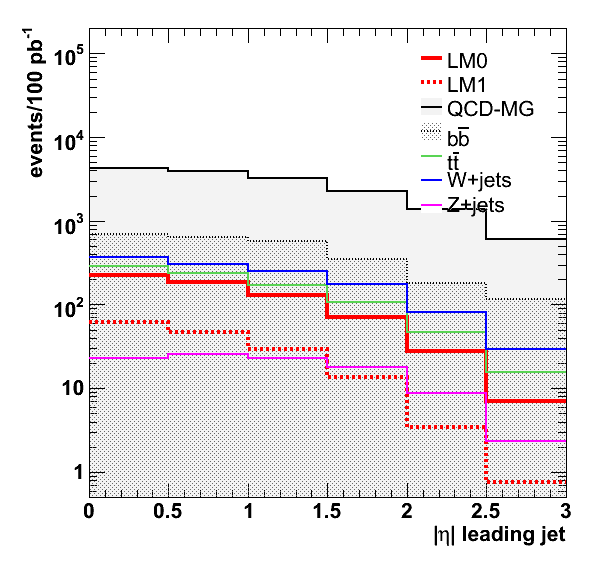
\includegraphics[scale=0.38]{./plots/JetEta.png}} 
\end{minipage}
\begin{minipage}[b]{0.5\linewidth}
\centering
{\label{fig:$H_{T}$}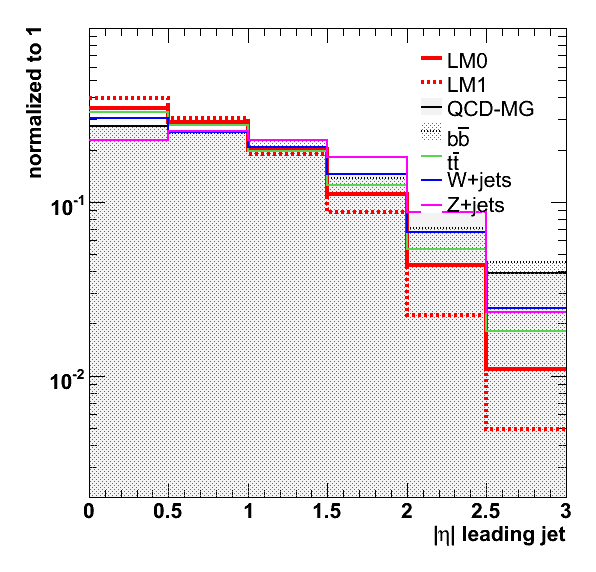
\includegraphics[scale=0.38]{./plots/JetEtaNorm.png}} 
\end{minipage}
\caption{\textit{The $|\eta|$ of the leading jet distribution, for the SUSY signal LM0 (solid red line), LM1 (dashed red line) and all the SM backgrounds superimposed.} }
\label{fig:jeteta}
\end{figure}


%\newpage
\subsection{The eta-$H_{T}$ kinematic method}

Figure \ref{fig:dists2} shows that a significant fraction of the SUSY signal is present high $H_{T}$ values.  As shown in the previous section, the $\alpha_T$ variable is very powerful in separating the signal and background events in two regions.  The QCD (and $b\bar{b}$) backgrounds can be controlled and, in fact, can be totally rejected by requesting that events satisfy $\alpha_{T}>0.55$. The above, plus the different eta dependence between signal and SM background samples, lead to establish the following analysis strategy.

Fisrt, we introduce the variable $R_{\alpha_T}$ which is defined as the ratio of the number of events passing the $\alpha_T$ cut over the number of events failing it:
\bea
R_{\alpha T} = \frac{N(\alpha_{T}>0.55)}{N(\alpha_{T}<0.55)}
\eea

We then study the behavior of $R_{\alpha T}$ as a function of the leading jet $|\eta|$.  This is done in different regions of $H_T$: it is expected that at low values of $H_T$ the ratio will be dominated by Standard Model processes, whereas at high values the SUSY signal will be relatively more prominent.  The basic idea is, therefore, to establish a different behavior of $R_{\alpha T}$ vs $|\eta|$ as we move from the background-dominated region (low-$H_T$) to the potentially signal-rich region (high $H_T$).

The QCD and $b\bar{b}$ backgrounds are expected to give R$_{aT}$ values of zero. Therefore, we study the effect of the remaining backgrounds, - $t\bar{t}$+jets and W+jets -, with a sizable amount of events above the $a_{T}$ cut. Figure \ref{fig:bkgsep} shows the distribution of R$_{aT}$ as a function of the leading jet $|\eta|$ for the QCD + $t\bar{t}$ (left) and QCD + W backgrounds (right), after requesting events with $H_T>$350~GeV. A slight slope - towards central values - tends to be visible in this $H_{T}$ region. In figure \ref{fig:bkgsep}, right, the point in the  $2< |\eta| < 2.5$ bin, which shows an upward fluctuation by more than one sigma, is due to event weighting effect (from the QCD sample). R$_{aT}$, after combining all the SM backgrounds, gives a flatish distribution as a function of $|\eta|$ for all $H_{T}$ bins, as shown in figure \ref{fig:id1}. 
       
Figure \ref{fig:id2} shows the R$_{aT}$ distribution for the background-plus-LM0 (left) and background-plus-LM1 (right) scenarios, respectively, for three different $H_{T}$ bins ([250,350], [350,inf] and [450,inf]). A rough comparison of the two scenarios, background-only and signal-plus-back- \\ ground, shows significant difference between them, as the $H_{T}$ threshold becomes higher.  

\begin{figure}[h!]
\begin{minipage}[b]{0.5\linewidth}
\centering
{\label{fig:m$H_{T}$ov$H_{T}$}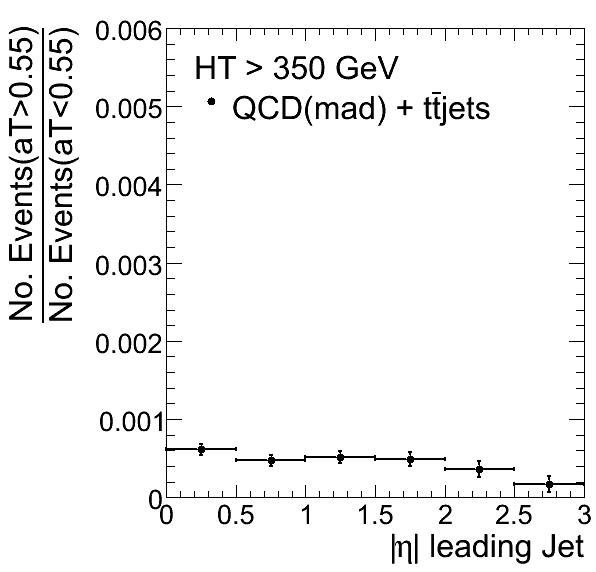
\includegraphics[scale=0.38]{./plots/RaT-TTbarVsQCD.png}} 
\end{minipage}
\begin{minipage}[b]{0.5\linewidth}
\centering
{\label{fig:$H_{T}$}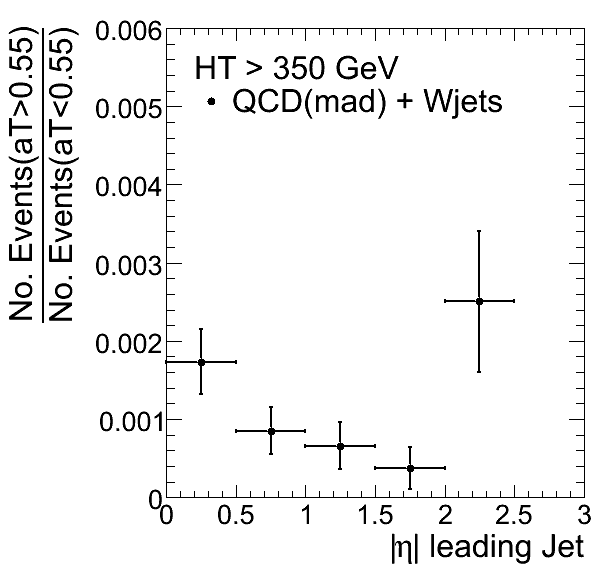
\includegraphics[scale=0.38]{./plots/RaT-WVsQCD.png}} 
\end{minipage}
\caption{\textit{The $R_{\alpha T}$ versus the leading jet $\eta$, for the $t\bar{t} + \textrm{jets}$ (left) and $W + \textrm{jets}$ (rig$H_{T}$), separately.} }
\label{fig:bkgsep}
\end{figure}

%\newpage
\begin{figure}[h!]
%\begin{minipage}[b]{0.5\linewidth} % A minipage that covers half the page
\centering
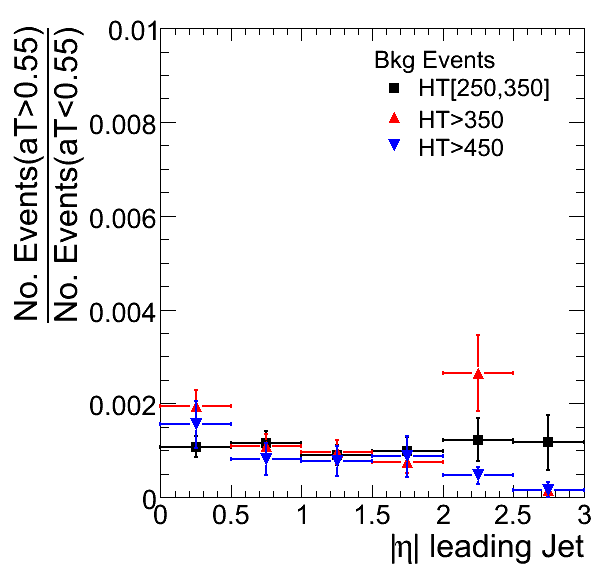
\includegraphics[scale=0.38]{./plots/RaT-Bkg.png}
%\end{minipage}
%\hspace{0.1cm} % To get a little bit of space between the figures
%\begin{minipage}[b]{0.5\linewidth}
%\centering
%\includegraphics[scale=0.38]{}
%\end{minipage}
\caption{\textit{The $R_{\alpha T}$ versus the leading jet $|\eta|$ for the SM background-only hypothesis, in three $H_{T}$ bins [250, 350], [350, inf], [450, inf].} }
\label{fig:id1}
\end{figure}

\begin{figure}[h!]
\begin{minipage}[b]{0.5\linewidth}
\centering
{\label{fig:aT}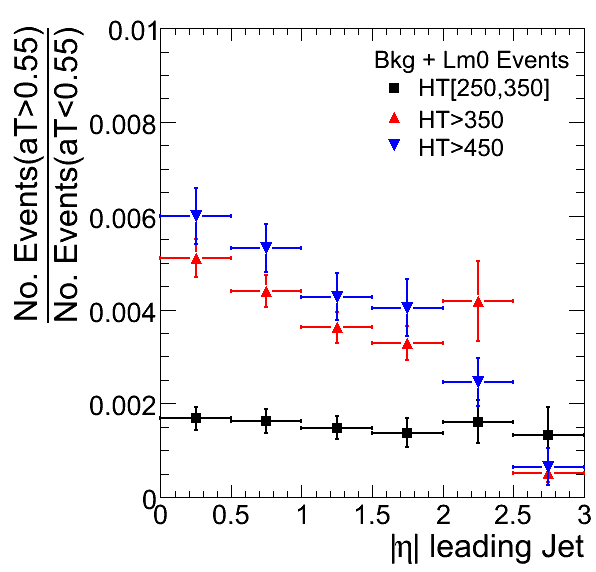
\includegraphics[scale=0.38]{./plots/RaT-LM0.png}} 
\end{minipage}
\begin{minipage}[b]{0.5\linewidth}
\centering
{\label{fig:m$H_{T}$}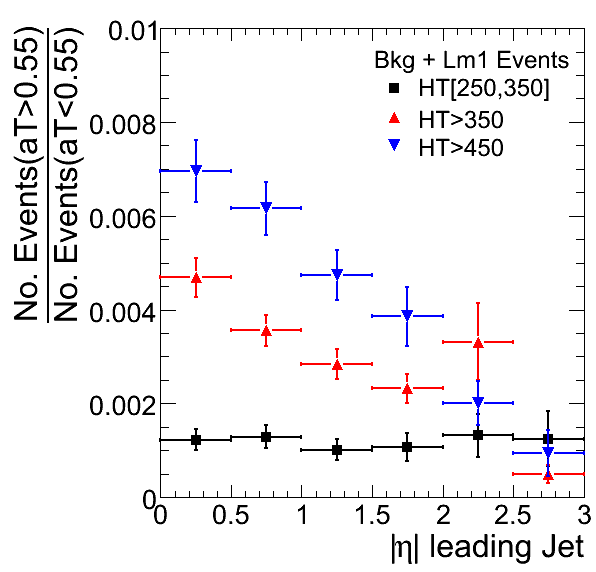
\includegraphics[scale=0.38]{./plots/RaT-LM1.png}} 
\end{minipage}
\caption{\textit{The $R_{\alpha T}$ versus the leading jet $|\eta|$ for the SUSY signal plus SM background hypothesis, in three $H_{T}$ bins [250, 350], [350, inf], [450, inf].} }
\vspace{5mm}
\label{fig:id2}
\end{figure}

\begin{comment}
\begin{figure}[h!]
\begin{minipage}[b]{0.5\linewidth} % A minipage that covers half the page
\centering
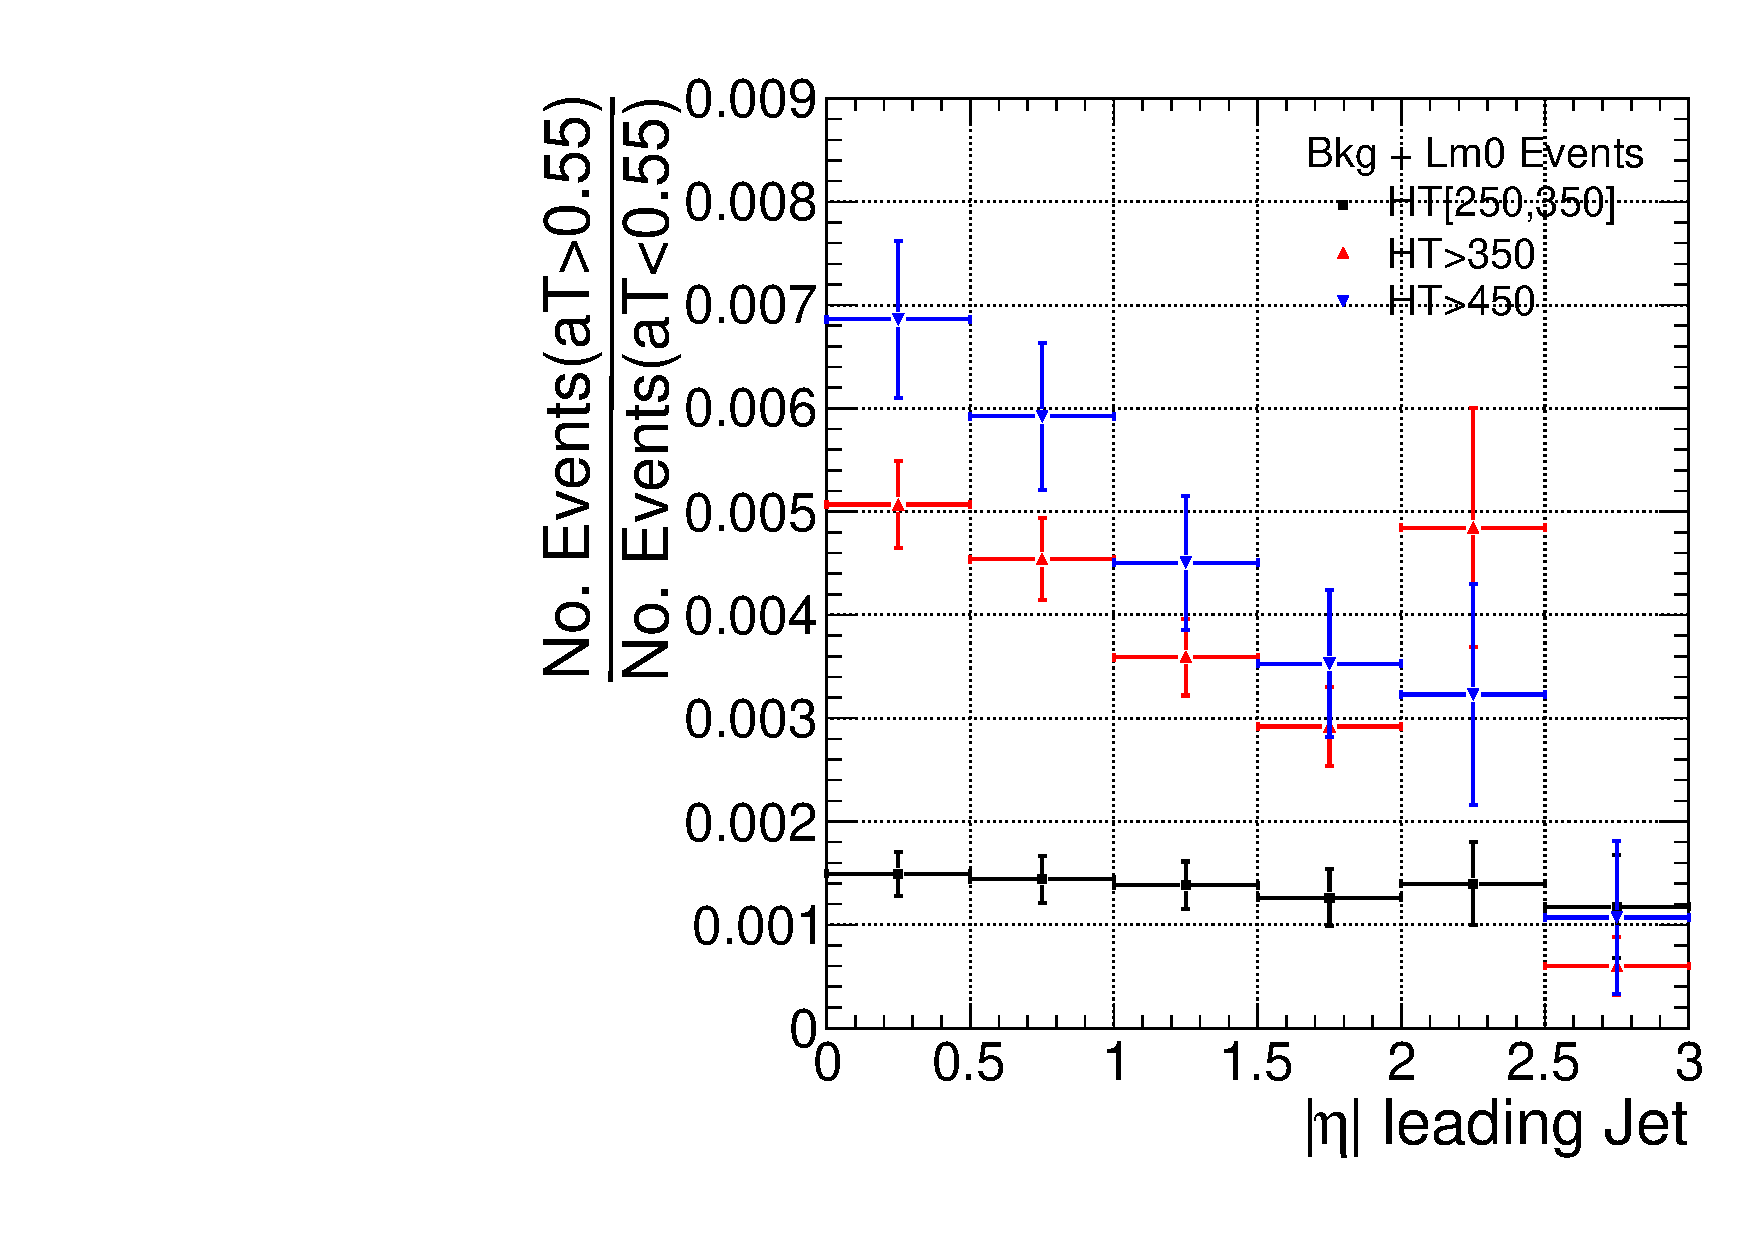
\includegraphics[scale=0.38]{./plots/aT-NT7-Lm0-MCerr}
\end{minipage}
\hspace{0.1cm} % To get a little bit of space between the figures
\begin{minipage}[b]{0.5\linewidth}
\centering
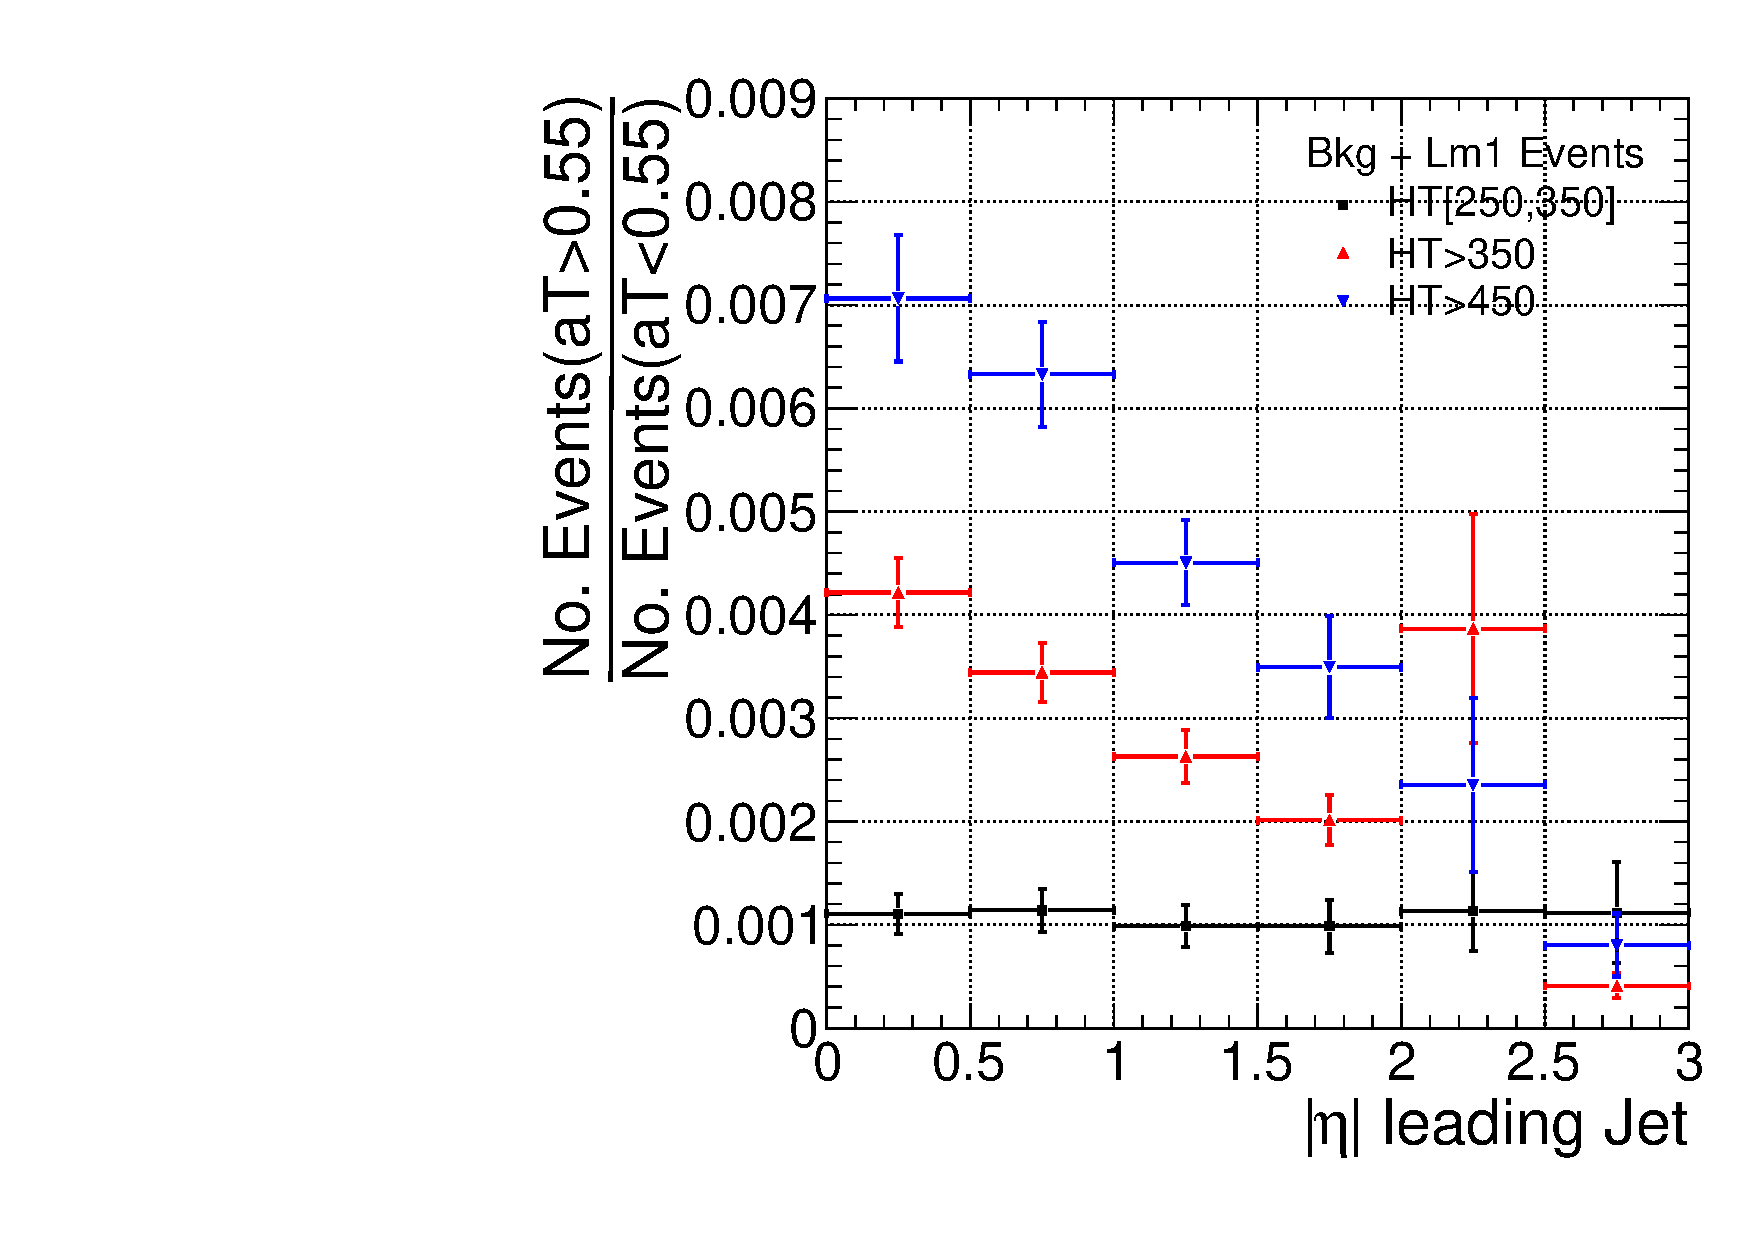
\includegraphics[scale=0.38]{./plots/aT-NT7-Lm1-MCerr}
\end{minipage}
\caption{\textit{The $R_{\alpha T}$ versus the leading jet $\eta$ for the SUSY signal plus SM background hypothesis, in three $H_{T}$ bins [250, 350], [350, inf], [450, inf].} }
\vspace{5mm}
\label{fig:id3}
\end{figure}
\end{comment}

%\clearpage

\subsection{Fitting $R_{\alpha T}$ vs eta}

This section describes an attempt to quantify the procedure of establishing a New Physics deviation from the SM background. A first method is tried by fitting the distributions of RaT vs the $|\eta|$ of the leading jet with a 1st degree polynomial ($p0 + p1 \cdot |\eta|$) using the $\chi^{2}$ method. The parameters of the fit, intercept and slope, for the background-only, as well as the signal-plus-background (background-plus-LM0 and background-plus-LM1) hypotheses have been plotted in bins of $H_{T}$ on figure ~\ref{fig:sum1}. One can easily observe the following:
\begin{enumerate}
 \item The background-only scenario shows flat distributions for both parameters as a function of $H_{T}$, which justifies the assumption of a constant RaT vs $|\eta|$. Instead, the fitting curves for both SUSY scenarios get an increasing incline as the $H_{T}$ threshold rises, leading to a clear distinguish from the background-only case.

\item Two regions in $H_{T}$ can be defined, depending on whether the SUSY signal is either suppressed or pronounced. A very first approach is to select the region with $H_{T}$ threshold below 300 GeV as the ``control region'' and the region $H_{T}>300$~GeV as the ``signal enriched'' region. By this technique and taking into account the flatness of the background distribution, we gain the advantage of estimating the background contribution directly from the data without using any MC-driven methods. We estimate the contribution from the control region and then extrapolate to higher $H_{T}$ regions. This leads inevitably to an over-estimation of the background, which still itself gives a ``safety factor'' which is important when dealing with early data.
\end{enumerate}

\begin{figure}[h!]
\begin{minipage}[b]{0.5\linewidth}
\centering
{\label{fig:m$H_{T}$ov$H_{T}$}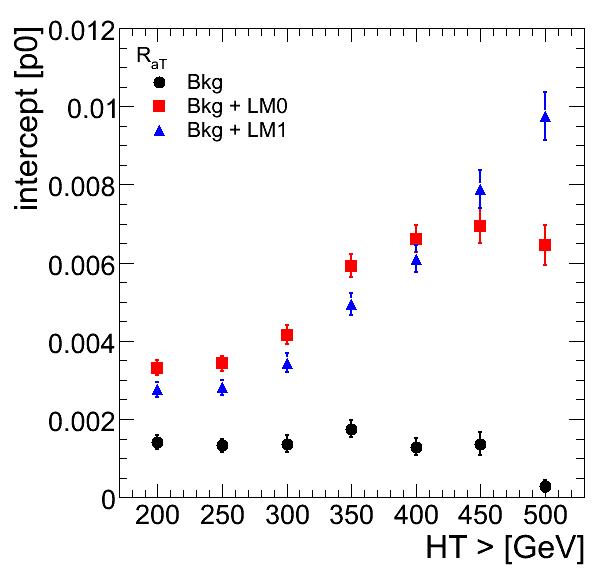
\includegraphics[scale=0.38]{./plots/aT-p0.png}} 
\end{minipage}
\begin{minipage}[b]{0.5\linewidth}
\centering
{\label{fig:$H_{T}$}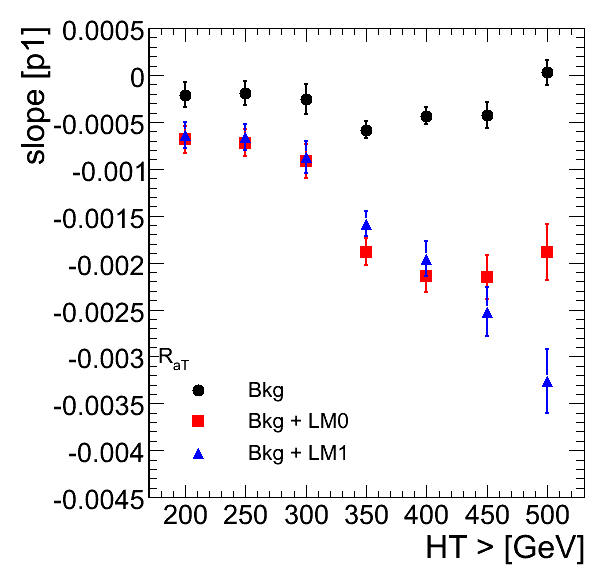
\includegraphics[scale=0.38]{./plots/aT-p1.png}} 
\end{minipage}
\caption{\textit{The fit to the $R_{\alpha T}$ vs $|\eta|$ curves, with a one-degree polynomial $f(|\eta|)= p0 + p1 \cdot |\eta|$, in bins of the $H_{T}$. Left figure shows the intercept ($p0$) values, and rig$H_{T}$ figure shows the slope ($p1$) values, in each $H_{T}$ bin, as extracted from the fit. Error bars assigned use the full MC statistics.  } }
\label{fig:sum1}
\end{figure}

\begin{figure}[h!]
\vspace{5mm}
\begin{minipage}[b]{0.5\linewidth}
\centering
{\label{fig:m$H_{T}$ov$H_{T}$}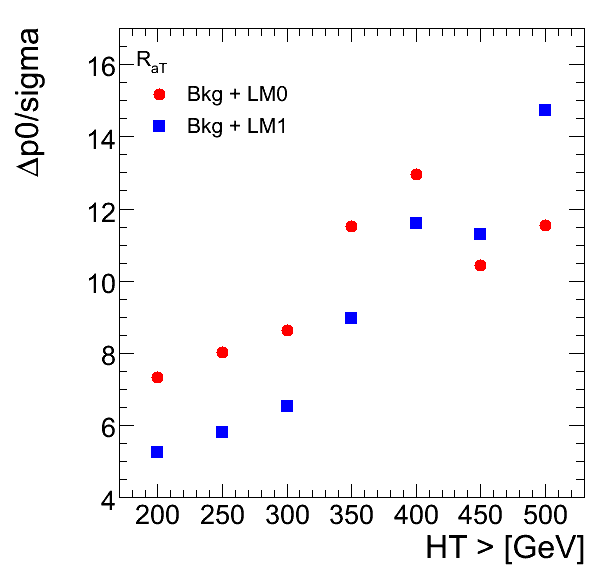
\includegraphics[scale=0.38]{./plots/aT-Dp0OvSigma.png}} 
\end{minipage}
\begin{minipage}[b]{0.5\linewidth}
\centering
{\label{fig:$H_{T}$}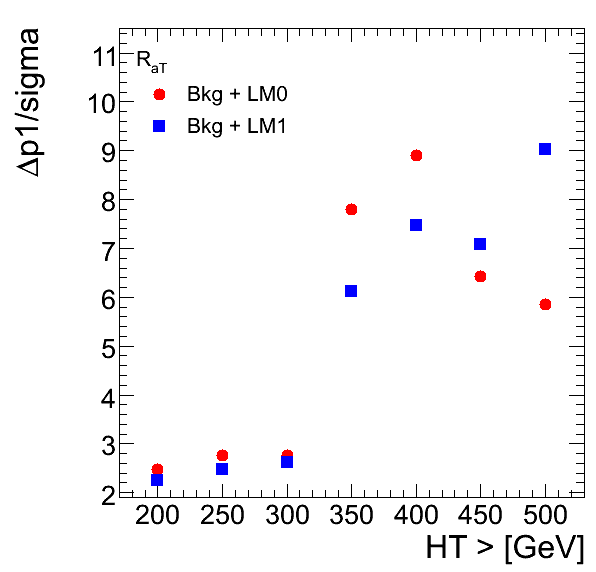
\includegraphics[scale=0.38]{./plots/aT-Dp1OvSigma.png}} 
\end{minipage}
\caption{\textit{A measure of the ``significance'' for establishing a SUSY deviation to the SM expectations: i) $\Delta p0 = p0_{fit}^{tot} - p0_{fit}^{bkg}$ - left figure - and $\Delta p1 = p1_{fit}^{tot} - p1_{fit}^{bkg}$ - rig$H_{T}$ figure -, divided by $\sigma = \sqrt{\sigma_{tot}^{2} + \sigma_{bkg}^{2}}$, in bins of $H_{T}$.  }}
\label{fig:sum2}
\end{figure}

Moving one step forward, we try to estimate the significance of the difference between the measured parameters (p0 and p1) with the presence of signal and the expected values in the background-only case. Thus, we calculate the quantity $\Delta p_{i} / sigma$, where:
\begin{eqnarray}
\Delta p_{i} = p_{i, fit}^{tot} - p_{i_fit}^{bkg},  \\
\sigma =  \sqrt{ (\delta (p_{i, fit}^{tot}))^{2} + (\delta (p_{i, fit}^{bkg}))^{2} } 
\end{eqnarray}
with the index $i$ corresponding to the two parameters of the fitting function.
<<<<<<< deviation.tex
In figure 13 (a) and (b), we plot this quantity for different HT bins, for the parameters p0 and p1 respectively, testing the bkg+LM0 and bkg+LM1 scenarios. When dealing with real data, the parameter values and the corresponding errors for the background-only case will be taken directly from the ``control region''. The difference in the intercept between the signal-plus-background and background-only cases, is more than 5 sigma in the low HT regions, and gets bigger, as expected, for higher HT thresholds. The difference in the slope though, becomes more important (above 5 sigma) for HT values above 350 GeV. This reinforces the assumption of selecting the region with $H_{T}<300$~GeV as a ``control region''.

\subsection{Alternatives variables to HT}
HT was chosen for this method as SM processes dominate in the low region, and potential SUSY signal in the higher region. Another typical observables that exhibits this behaviour is the effective mass, $M_{eff}$, for which the distribution is shown in Figure . We repeat the previous analysis, using regions of $M_{eff}$ instead of H$_{T}$, for comparison, whilst having imposed a 350GeV cut on H$_{T}$.The plota in figure show the same deviation from background hypothesis as was seen for HT. The deviation is in this case more rapid though it is clearly dependent on the choice of Meff bins. Using the 


=======
In figure \ref{tab:sum2}, we plot this quantity for different $H_{T}$ bins, for the parameters p0 (left) and p1 (right) respectively, testing the background-plus-LM0 and background-plus-LM1 scenarios. When dealing with real data, the parameter values and the corresponding errors for the background-only case will be taken directly from the ``control region''. The difference in the intercept between the signal-plus-background and background-only cases, is more than 5 sigma in the low $H_{T}$ regions, and gets bigger, as expected, for higher $H_{T}$ thresholds. The difference in the slope though, becomes more important (above 5 sigma) for $H_{T}$ values above 350 GeV. This reinforces the assumption of selecting the region with $H_{T}<300$~GeV as a ``control region''.>>>>>>> 1.8


\section{Systematic uncertainties on signal efficiency \label{sec:systematics}}

The systematic uncertainties on the signal event yield are estimated
following in general the recipes discussed in ~\cite{RA1Paper} and are
split into two parts: theoretical uncertainties on the predicted cross
section of the different production processes (squark-squark,
squark-gluino, gluino-gluino) and experimental uncertainties on the
integrated luminosity and on the selection efficiency.

The experimental systematic uncertainties on the estimated signal
event yield are the uncertainty on the luminosity measurement
(6\%)~\cite{ref:lumi}, the effect of rejecting events with jets
pointing to masked ECAL regions (3\%)~\cite{RA1Paper}, the modelling
of the lepton and photon vetoes in the simulation
(2.5\%)~\cite{RA1Paper}, and the effect of the uncertainty in the jet
energy scale and resolution on the selection efficiency
(2.5\%)~\cite{RA1Paper,PAS-JME-10-010}.

The systematic uncertainties on the next-to-leading order (NLO) cross
section predictions due to the choice of the renormalization and
factorization scales combined with the uncertainties on the used
parton distribution functions amount to a 10\% systematic uncertainty.

These uncertainties are all included in the limit calculation.

\section{Summary}
\label{sec:Summary}

This study proposes two methods of data-driven QCD background estimation, and presents results from Monte Carlo and the first X pb$^{-1}$ of 7TeV data taken by CMS at the LHC. 

Following the promising results of studies into using the $\alpha_{T}$  kinematic variable in the single electron mode of SUSY searches, it is proposed that a suitable control sample in the distribution of this variable for predicting the QCD background could be obtained by inverting the $\Delta \phi$ and $\Delta \eta$ cuts in the electron selection criteria. 

The analysis uses Monte Carlo samples to perform a closure test on this method, first with a pure QCD sample, and then with W + jets contamination in the anti-selected control sample. The method proved unbiased between selected and anti-selected in these tests. 

The first look at this method under 7TeV collision data and corresponding Monte Carlo is also shown, with lowered selection to maximise available statistics.


%\newpage
%\section{Background estimation methods}

%\subsection{Data-driven background estimation for $W+jets$}

%\section{Summary}
%\label{sec:Summary}

\clearpage

%\appendix

%\newpage
%\bibliographystyle{plain}
%\bibliography{Bibliography}

\begin{thebibliography}{9}
\bibitem{data}{https://twiki.cern.ch/twiki/bin/view/CMS/ProductionSummer2009.}
\bibitem{mad}{J~Alwall et al., ``MadGraph/MadEvent v4: The New Web generation'', JHEP 09 (2007) 028, arXiv:0706.2334.}
\bibitem{lmx} {http://cmsdoc.cern.ch/cms/PRS/susybsm/msugra\_testpts/msugra\_testpts.html.}
\bibitem{susypat1} {https://twiki.cern.ch/twiki/bin/view/CMS/SusyPat.}
\bibitem{susypat2} {https://twiki.cern.ch/twiki/bin/view/CMS/SWGuidePAT.}
\bibitem{susypat}{https://twiki.cern.ch/twiki/bin/view/CMS/SusyPatLayer1.}
\bibitem{cc} {https://twiki.cern.ch/twiki/bin/view/CMS/SusyPatCrossCleaner.}
\bibitem{ICNT}{https://twiki.cern.ch/twiki/bin/view/CMS/SusyICFNtuple.}
\bibitem{ra4}{https://twiki.cern.ch/twiki/bin/view/CMS/SusyRA4SingleLeptonOrganization.}
\bibitem{elecid}{\bf{CMS AN-2008/082}}{\em``A cut based method for electron identification in CMS''.}
\bibitem{muonid}{\bf{CMS AN-2008/098}}{\em``Muon Identification in CMS''.}
\bibitem{vjets}{https://twiki.cern.ch/twiki/bin/view/CMS/VplusJets.}
\bibitem{iso}{Z.~Hatherell, G.~Karapostoli, M.~Pioppi, A.~Savin, A.~Sparrow, M.~Weinberg, {\em``Study of isolation properties of SUSY low-$p_{T}$ leptons.''}, CMS Analysis Note 2009/167.}
\bibitem{lisa}{L.~Randall and D.~Tucker-Smith, {\em``Dijet searches for Supersymmetry at the LHC''}, Phys. Rev. Lett. \bf{101} (2008) 221803, arXiv:0806.1049.}
\bibitem{njet}{H.~Flaecher, M.~Stoye, T.~Rommerskirchen, T.~Yetkin, T.~Whyntie, R.~Bainbridge, J.~Marrouche, {\em``Search for SUSY with exclusive n-jet events''}, CMS Analysis Note 2008/082. }
%\bibitem{elecid}{\bf{CMS AN-2008/082}}{\em``A cut based method for electron identification in CMS''}
%\bibitem{muonid}{\bf{CMS AN-2008/098}}{\em``Muon Identification in CMS''}
%  \bibitem {NOTE000} {\bf CMS Note 2005/000},
%    X.Somebody et al.,
%    {\em "CMS Note Template"}.
\end{thebibliography}

\newpage

\appendix
\section{Alternatives to the $\alpha_{T}$ approach}

Typical observables that separate SUSY signal from the background are $MH_{T}$ and $MH_{T}/H_{T}$. We repeat the same analysis as for the $R_{\alpha T}$ case. We estimate a cut value on $MH_{T}$ at 200 GeV which rejects (mainly) the QCD and $b\bar{b} + \textrm{jets}$ background, while this has a small impact on the SUSY signal. For the $MH_{T}/H_{T}$ observable, a cut value with similar effects is $0.4$. We then calculate the ratio $R_{MHT}$ and $R_{MHT/HT}$.  

Figure \ref{fig:app1} shows the $R_{MHT}$ versus the $|\eta|$ of the leading jet for the SM background only case, in three different $H_{T}$ bins. The dependence on $H_{T}$ value and $|\eta|$ of the leading jet is apparent. In figures~\ref{fig:app2}, we plot the $R_{MHT}$ value for the SUSY signal LM0 (left) and LM1 (right) respectively, plus the SM background, versus the $|\eta|$ of the leading jet. Again the signal case is more central than the background and clearly depends on the $H_{T}$ bin. 

The corresponding plots for $R_{MHT/HT}$ are plotted in figures ~\ref{fig:app3} and ~\ref{fig:app4}. The SM background case is quite similar to the $R_{\alpha T}$ case. The $R_{MHT/HT}$ has a small trend to more central values for higher HT bins. From the background-plus-signal plots, we conclude that $R_{MHT/HT}$ depends highly on the $H_{T}$ and the leading jet $\eta$. 

\begin{figure}[h!]
%\begin{minipage}[b]{0.5\linewidth} % A minipage that covers half the page
\centering
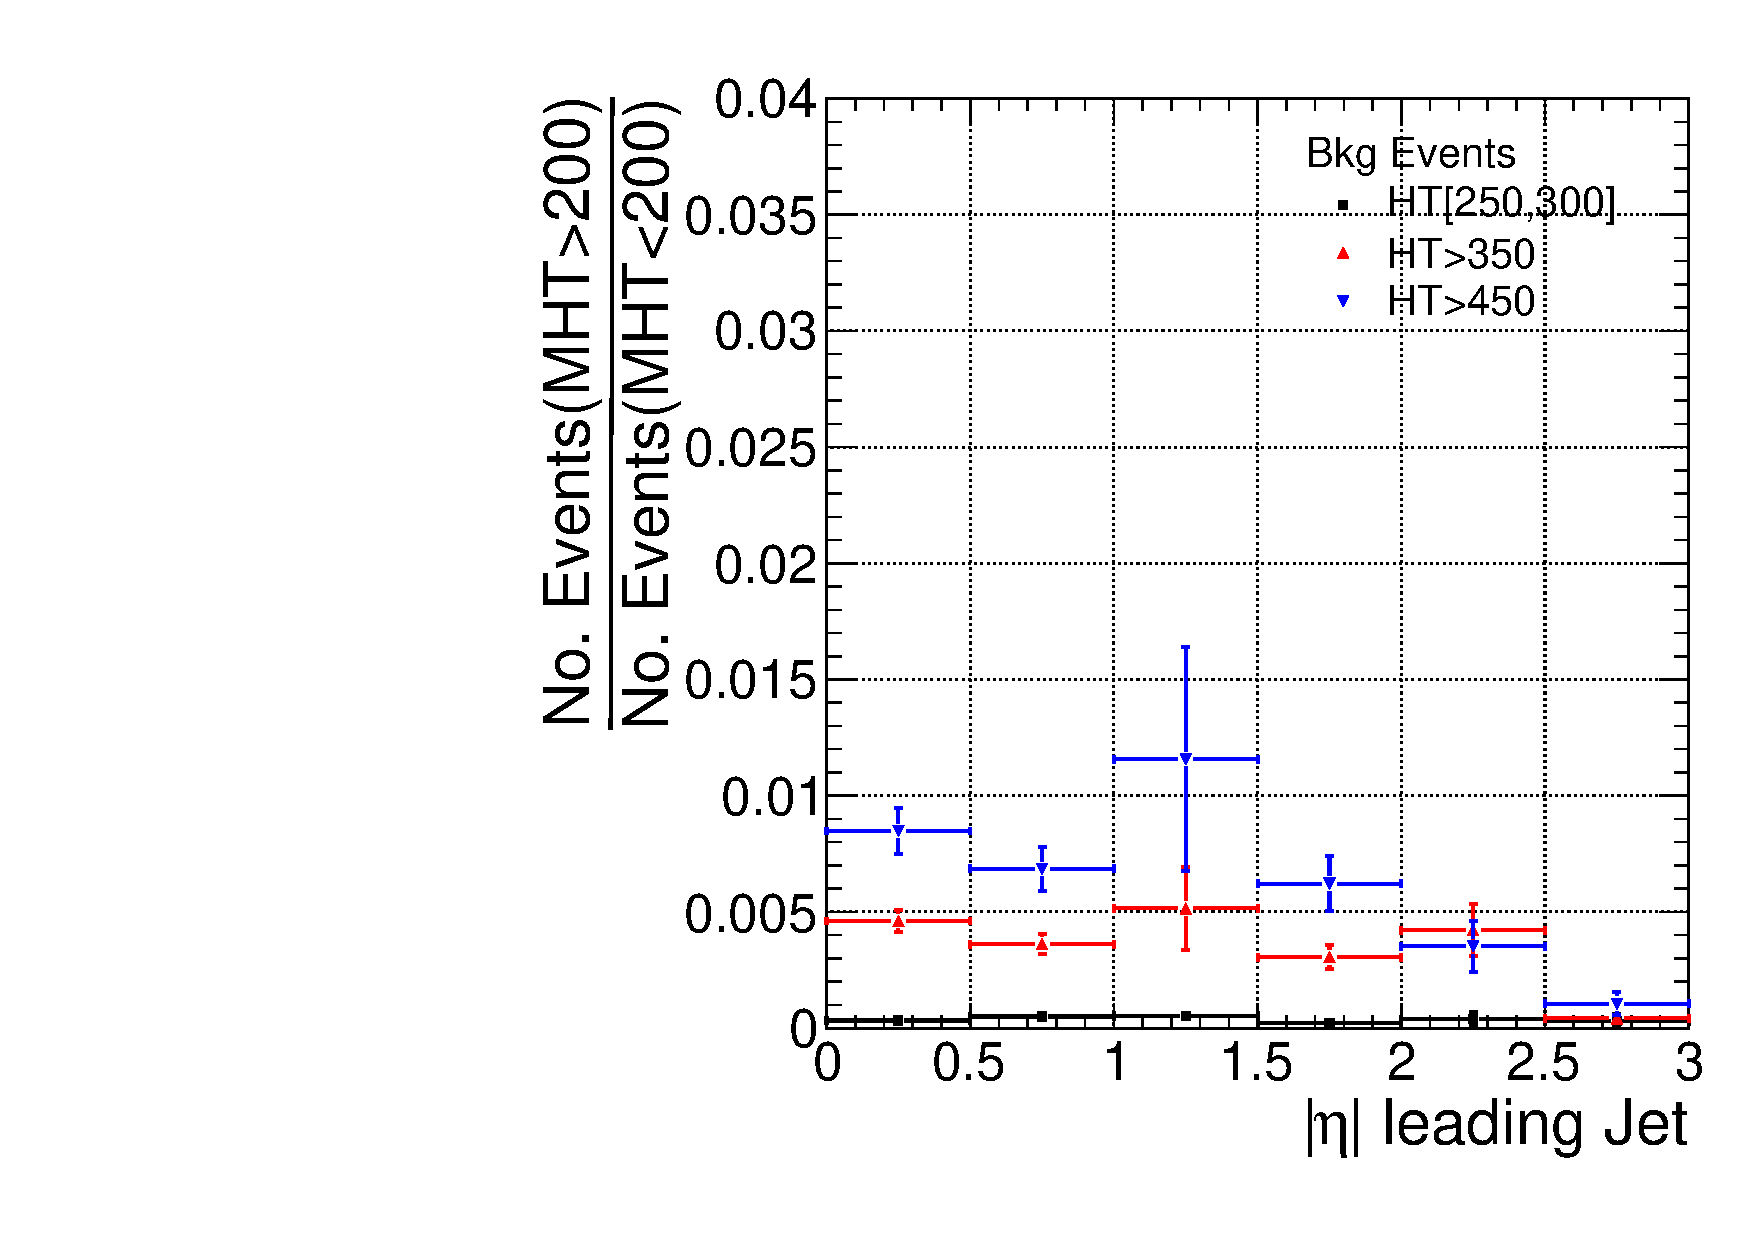
\includegraphics[scale=0.4]{./plots/MHT-NT7-Bkg-MCerr}
%\end{minipage}
%\hspace{0.1cm} % To get a little bit of space between the figures
%\begin{minipage}[b]{0.5\linewidth}
%\centering
%\includegraphics[scale=0.4]{}
%\end{minipage}
\caption{\textit{The $R_{MHT}$ versus the leading jet $|\eta|$ for the SM background-only hypothesis, in three $H_{T}$ bins [250, 350], [350, inf], [450, inf].} }
\label{fig:app1}
\end{figure}

\begin{figure}[h!]
\begin{minipage}[b]{0.5\linewidth}
\centering
{\label{fig:aT}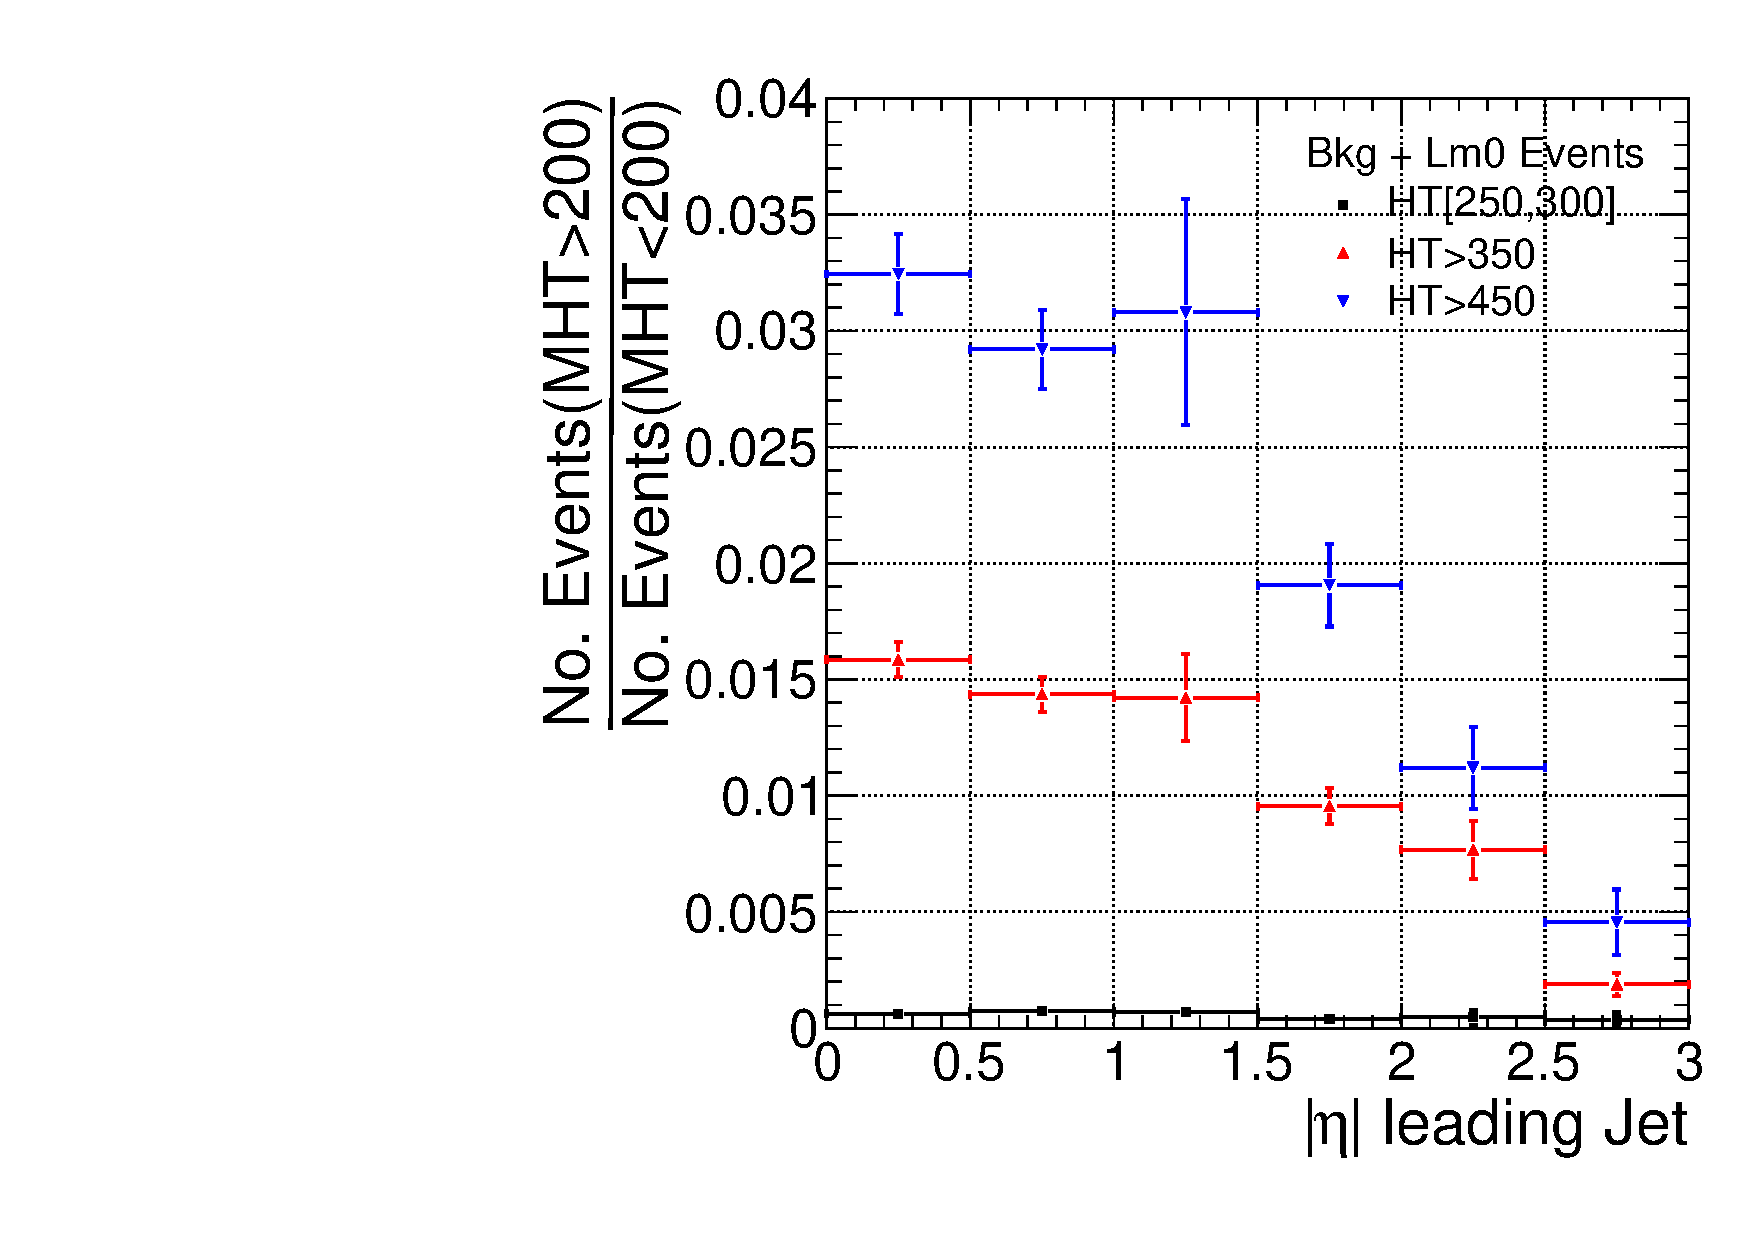
\includegraphics[scale=0.4]{./plots/MHT-NT7-Lm0-MCerr}} 
\end{minipage}
\begin{minipage}[b]{0.5\linewidth}
\centering
{\label{fig:mht}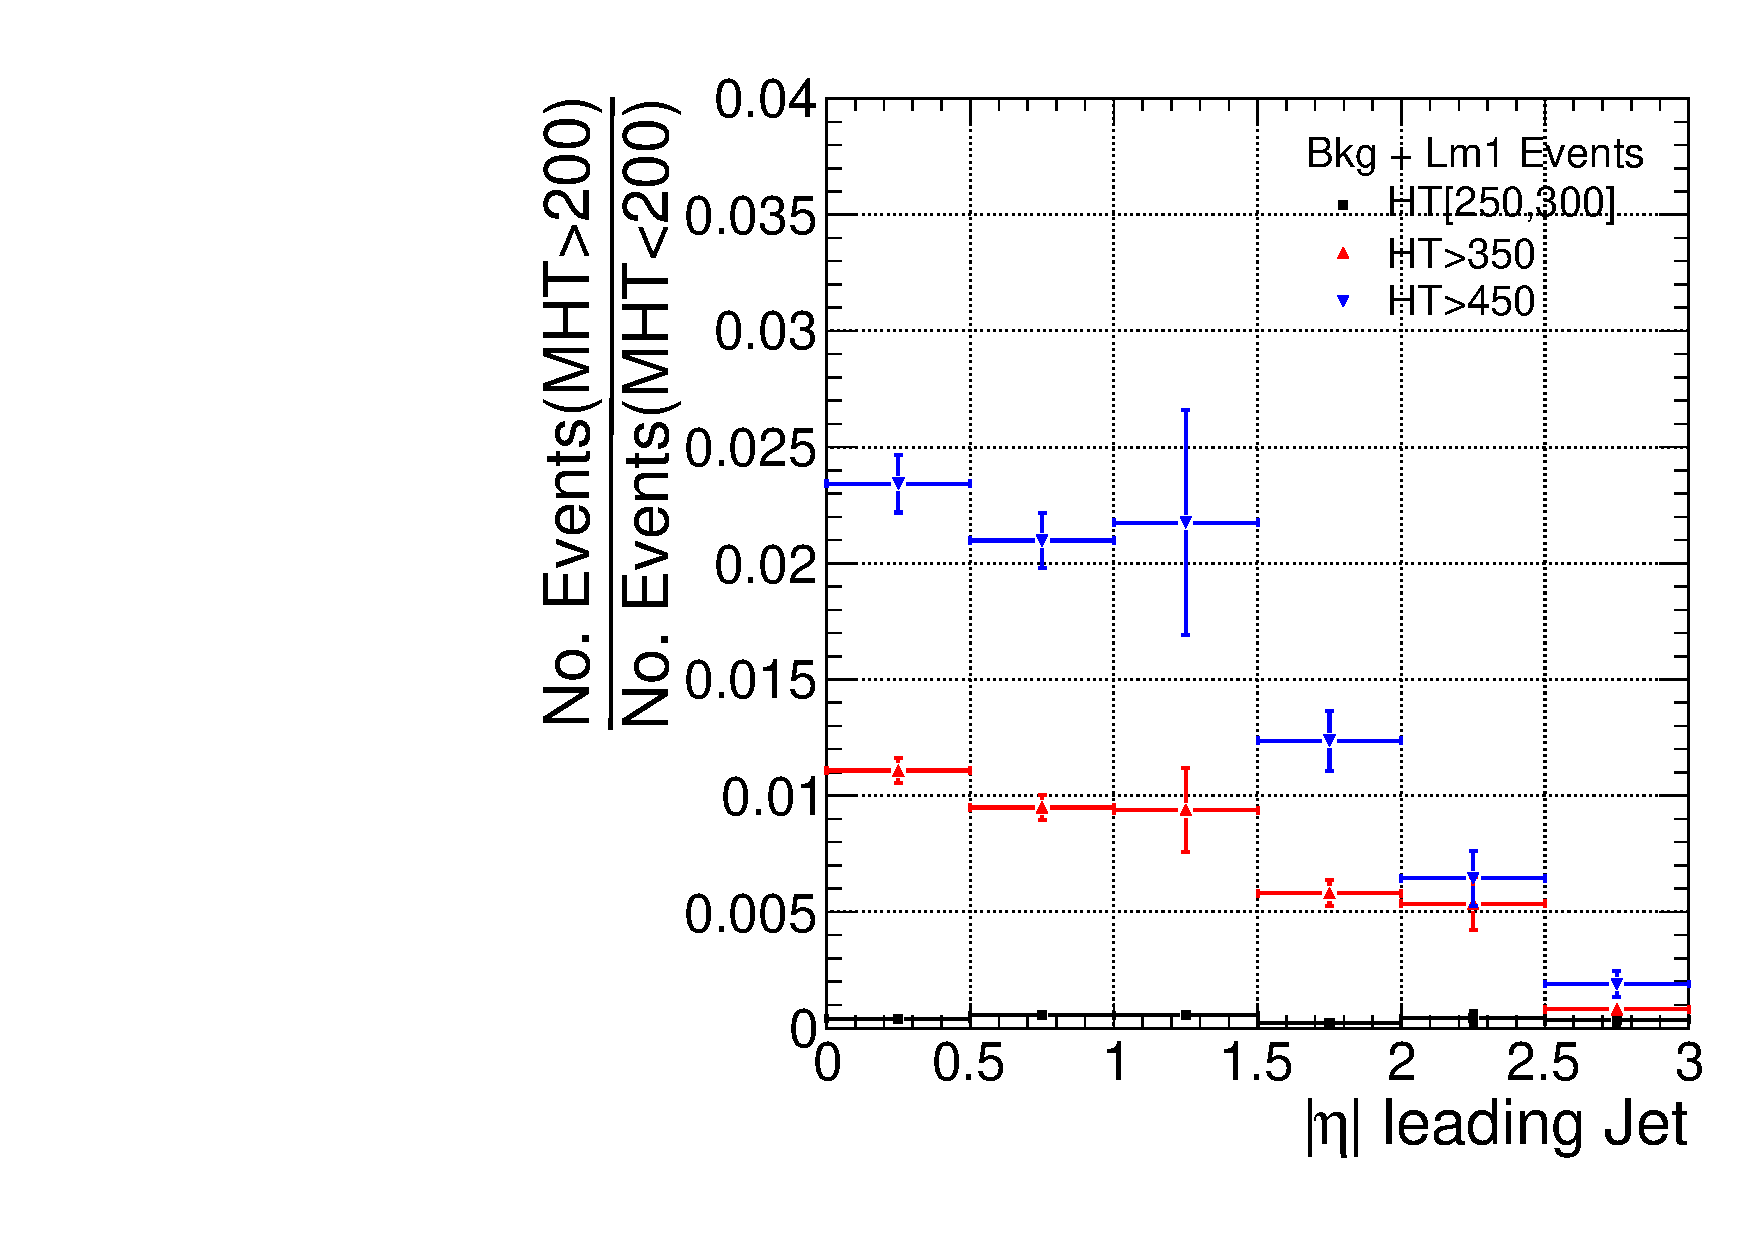
\includegraphics[scale=0.4]{./plots/MHT-NT7-Lm1-MCerr}} 
\end{minipage}
\caption{\textit{The $R_{MHT}$ versus the leading jet $|\eta|$ for the SUSY signal plus SM background hypothesis, in three $H_{T}$ bins [250, 350], [350, inf], [450, inf].} }
\label{fig:app2}
\end{figure}

\begin{figure}[h!]
%\begin{minipage}[b]{0.5\linewidth} % A minipage that covers half the page
\centering
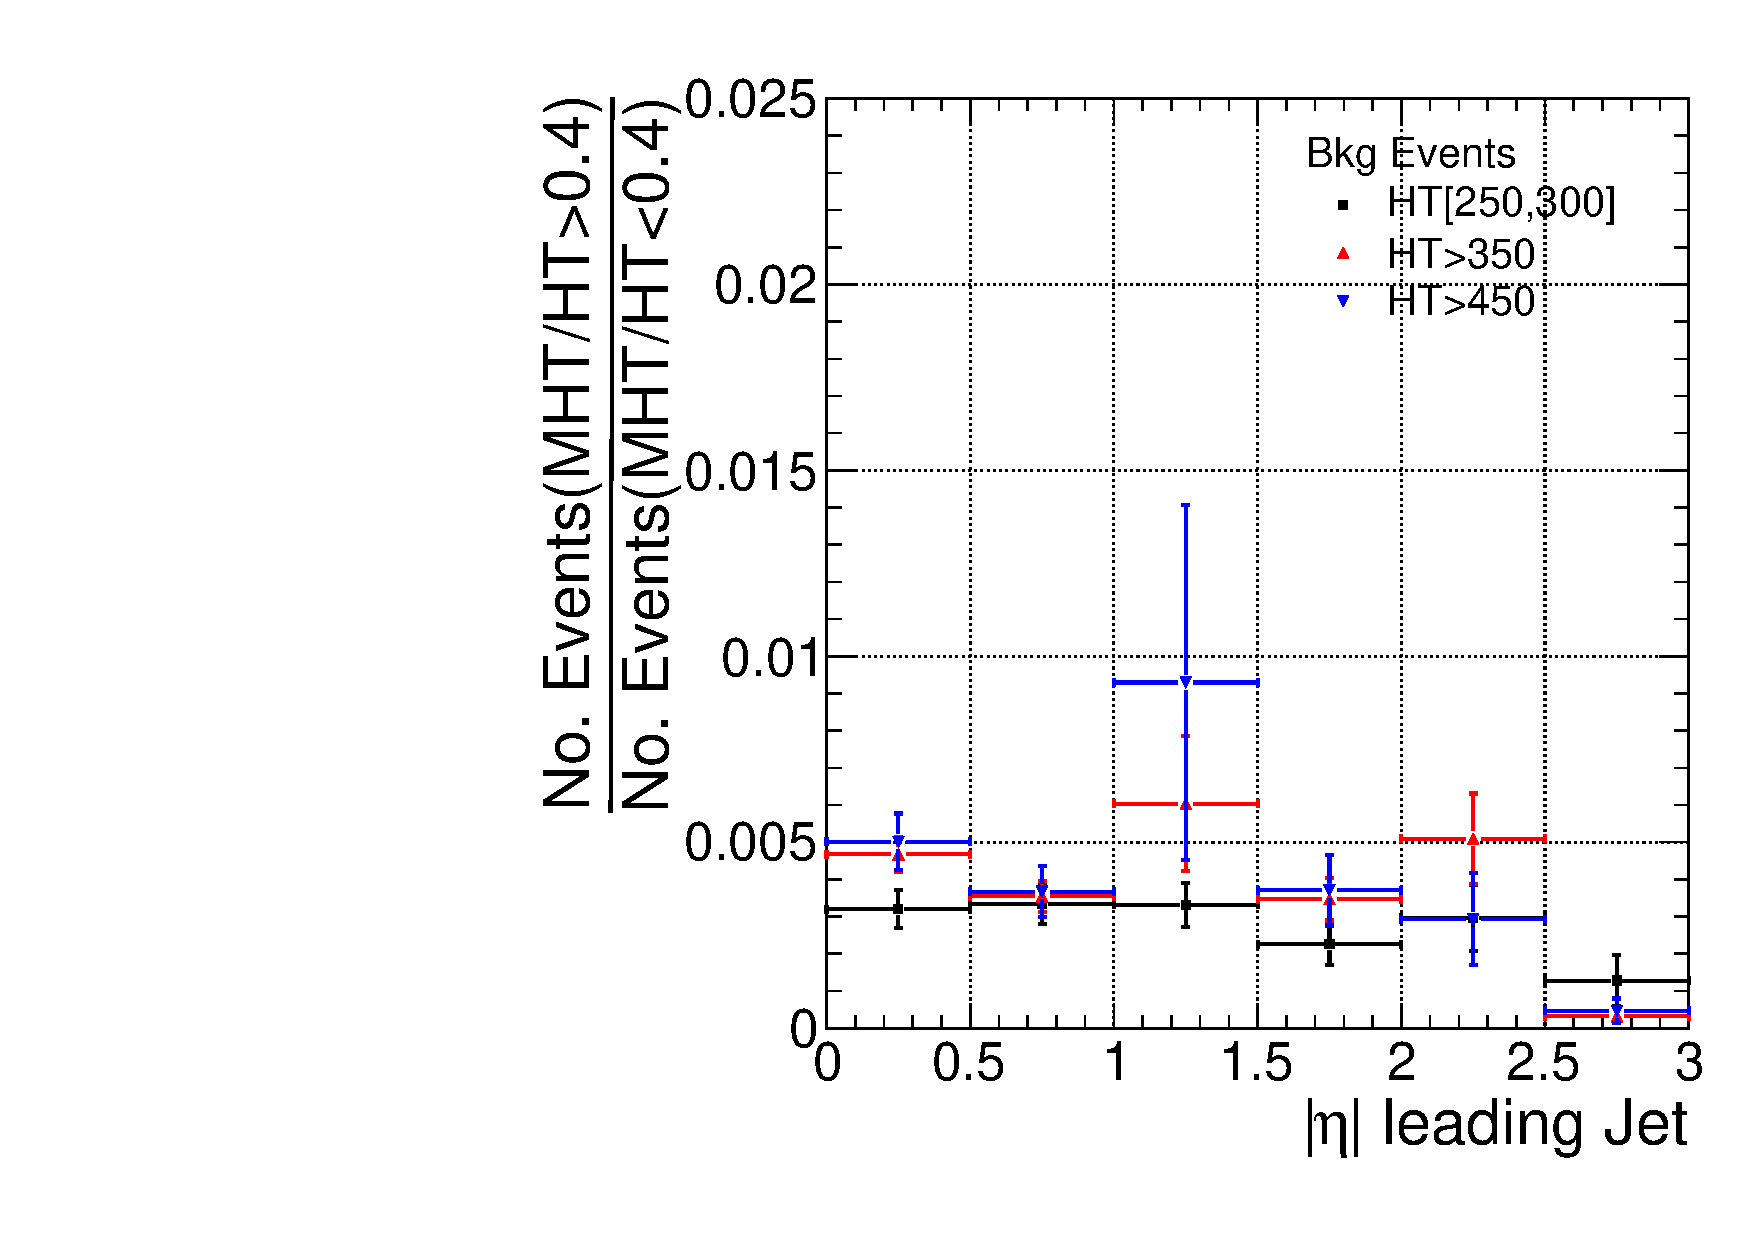
\includegraphics[scale=0.4]{./plots/MHTovHT-NT7-Bkg-MCerr}
%\end{minipage}
%\hspace{0.1cm} % To get a little bit of space between the figures
%\begin{minipage}[b]{0.5\linewidth}
%\centering
%\includegraphics[scale=0.4]{}
%\end{minipage}
\caption{\textit{The $R_{MHT/HT}$ versus the leading jet $|\eta|$ for the SM background-only hypothesis, in three $H_{T}$ bins [250, 350], [350, inf], [450, inf].} }
\label{fig:app3}
\end{figure}

\begin{figure}[h!]
\begin{minipage}[b]{0.5\linewidth}
\centering
{\label{fig:aT}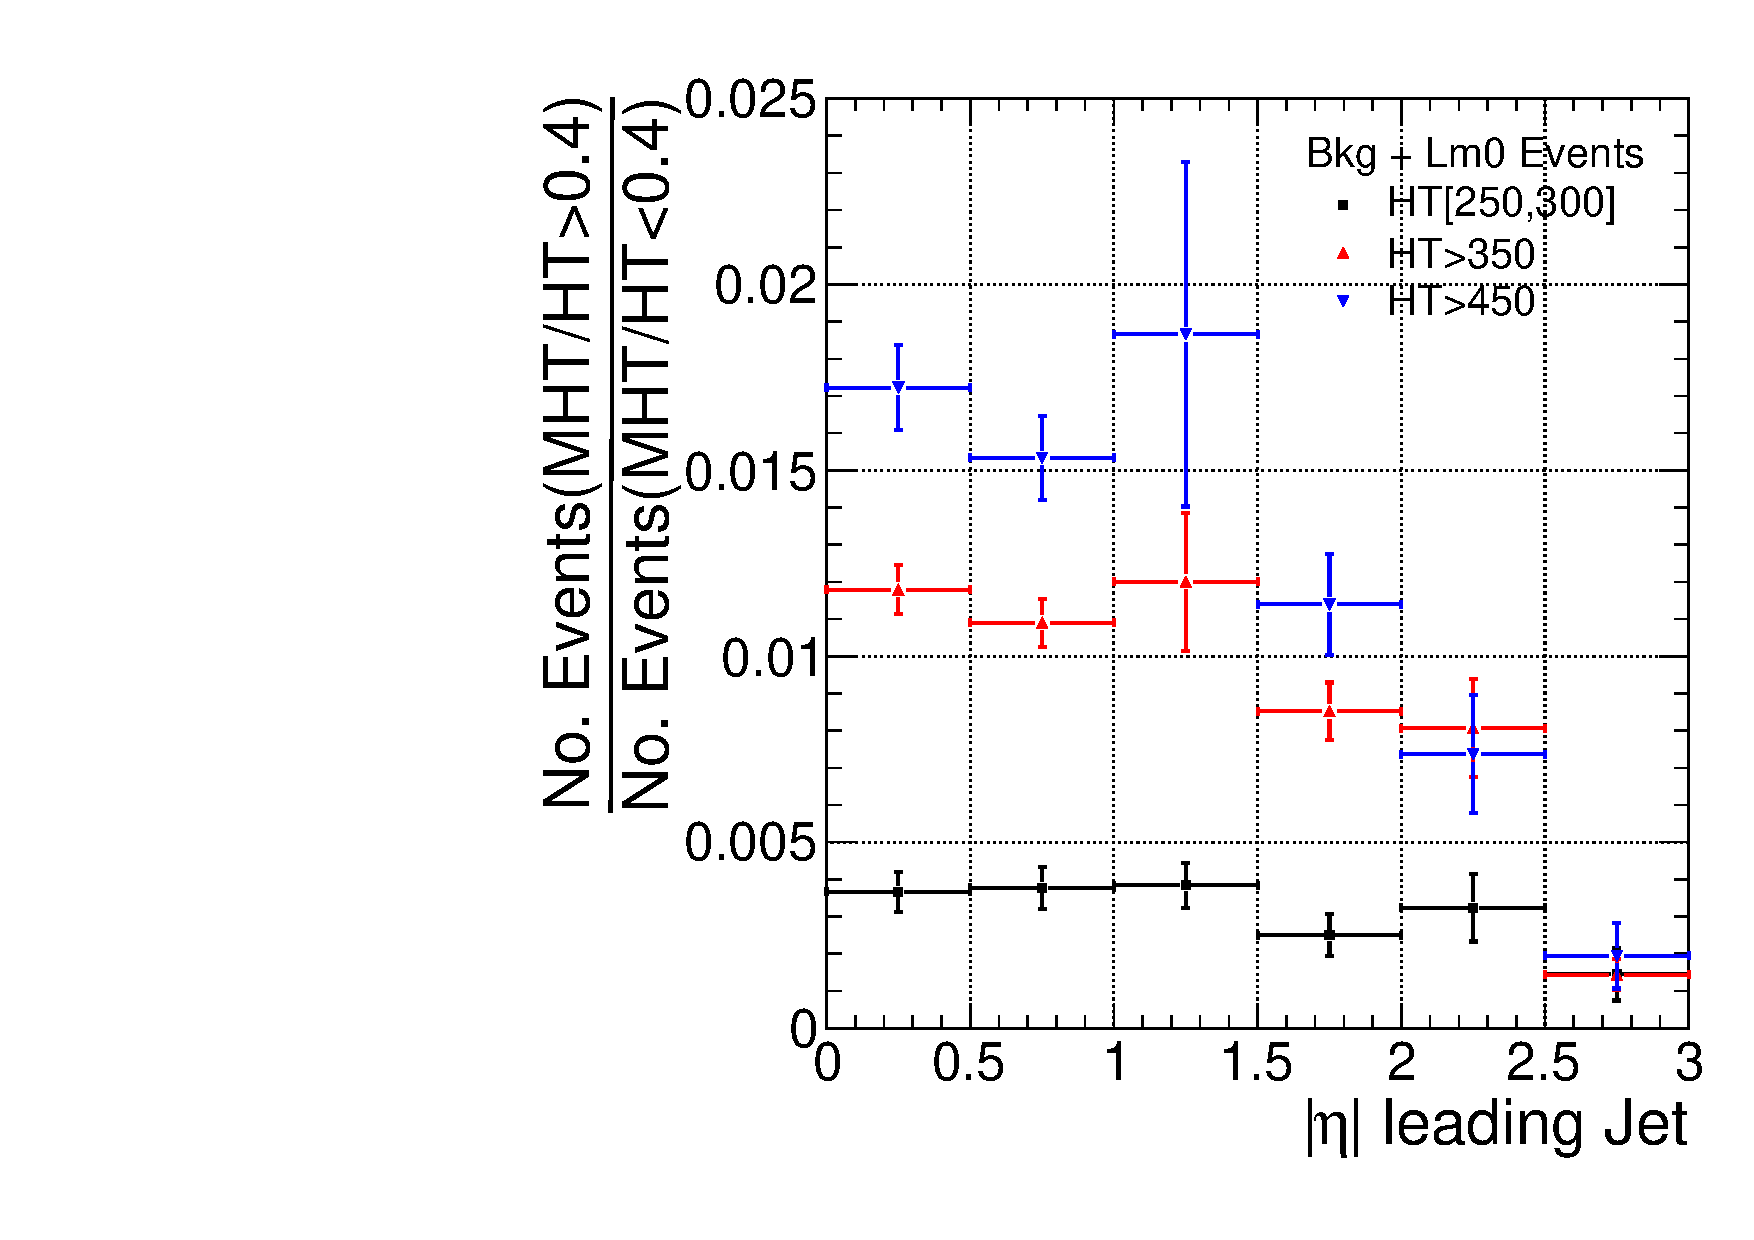
\includegraphics[scale=0.4]{./plots/MHTovHT-NT7-Lm0-MCerr}} 
\end{minipage}
\begin{minipage}[b]{0.5\linewidth}
\centering
{\label{fig:mht}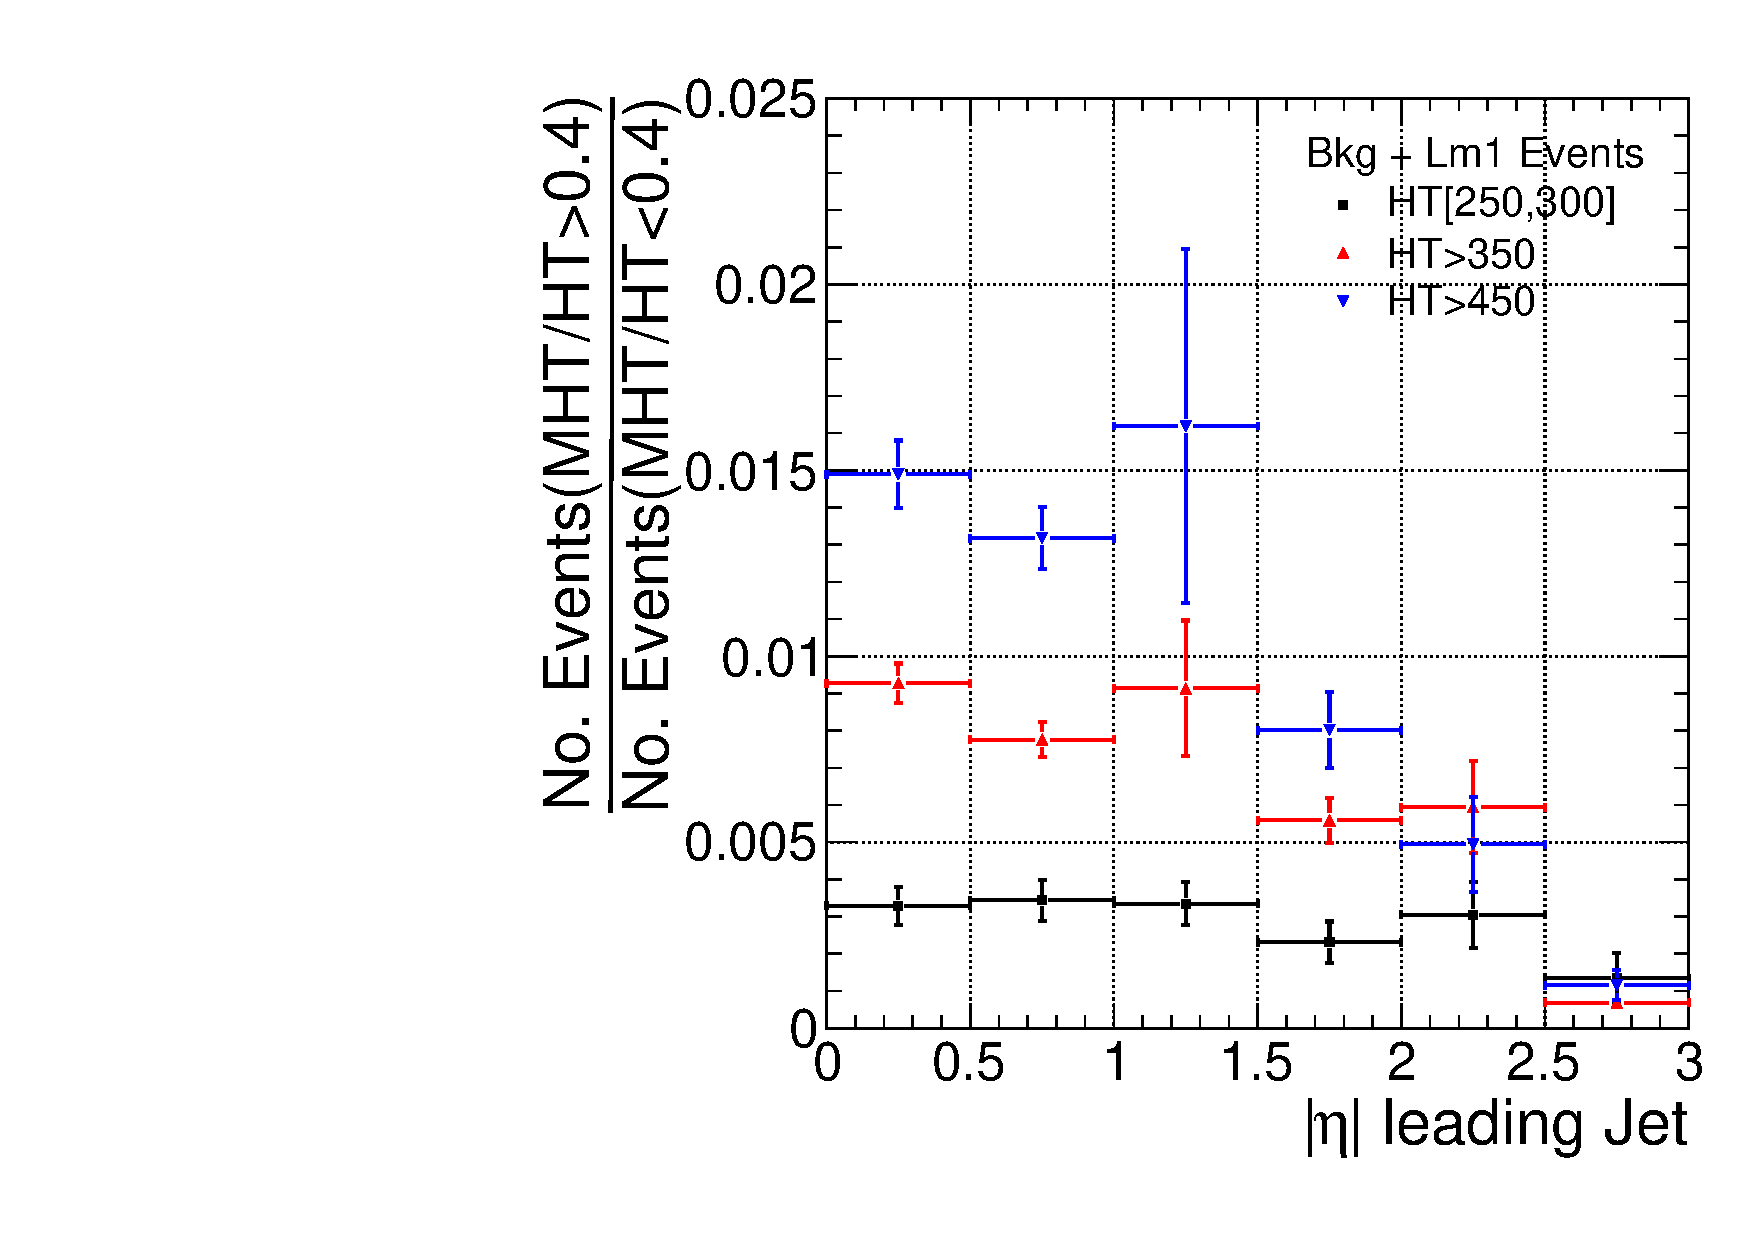
\includegraphics[scale=0.4]{./plots/MHTovHT-NT7-Lm1-MCerr}} 
\end{minipage}
\caption{\textit{The $R_{MHT/HT}$ versus the leading jet $|\eta|$ for the SUSY signal plus SM background hypothesis, in three $H_{T}$ bins [250, 350], [350, inf], [450, inf].} }
\label{fig:app4}
\end{figure}

\begin{comment}
\begin{figure}[h!]
%\begin{minipage}[b]{0.5\linewidth} % A minipage that covers half the page
\centering
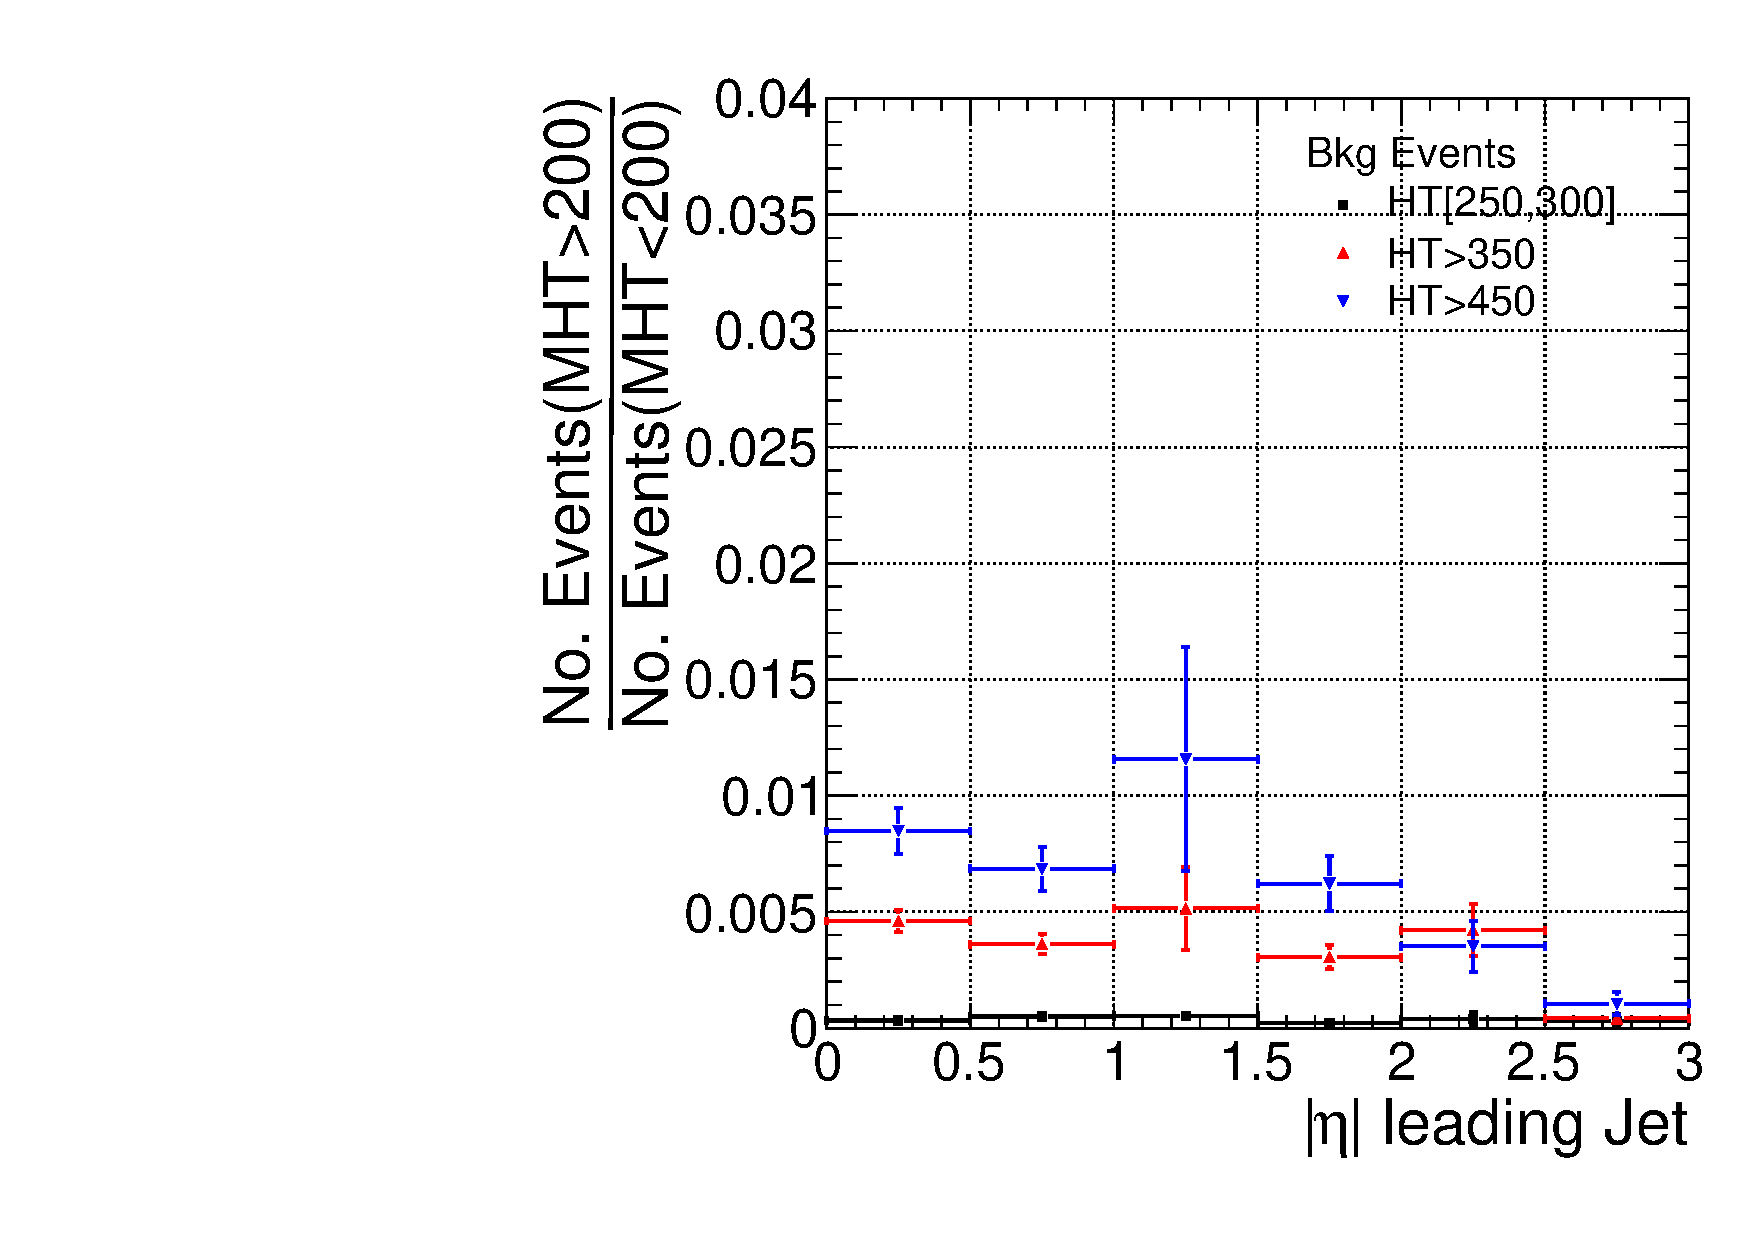
\includegraphics[scale=0.4]{./plots/MHT-NT7-Bkg-MCerr}
%\end{minipage}
%\hspace{0.1cm} % To get a little bit of space between the figures
%\begin{minipage}[b]{0.5\linewidth}
%\centering
%\includegraphics[scale=0.4]{}
%\end{minipage}
%  \caption{ }
\label{fig:app6}
\end{figure}
\begin{figure}[h!]
\begin{minipage}[b]{0.5\linewidth} % A minipage that covers half the page
\centering
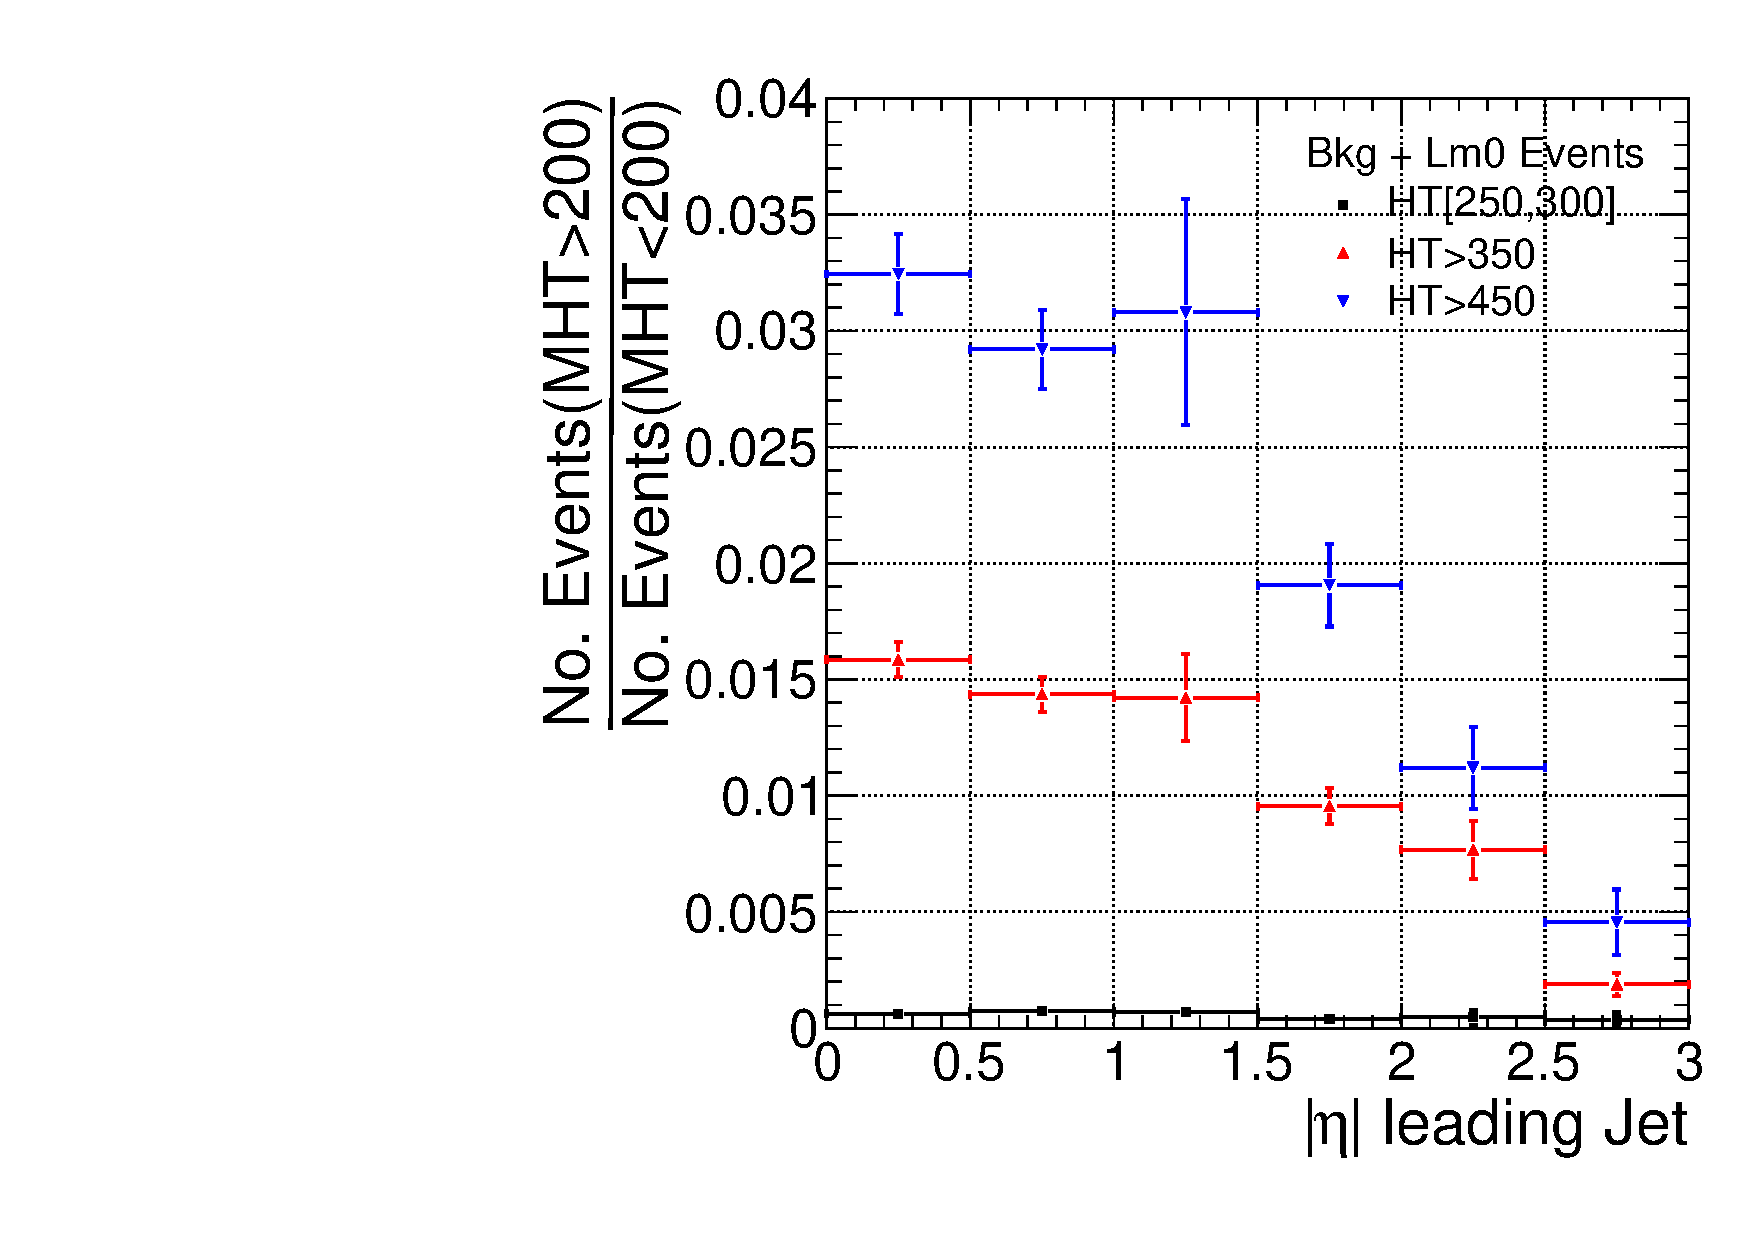
\includegraphics[scale=0.4]{./plots/MHT-NT7-Lm0-MCerr}
\end{minipage}
\hspace{0.1cm} % To get a little bit of space between the figures
\begin{minipage}[b]{0.5\linewidth}
\centering
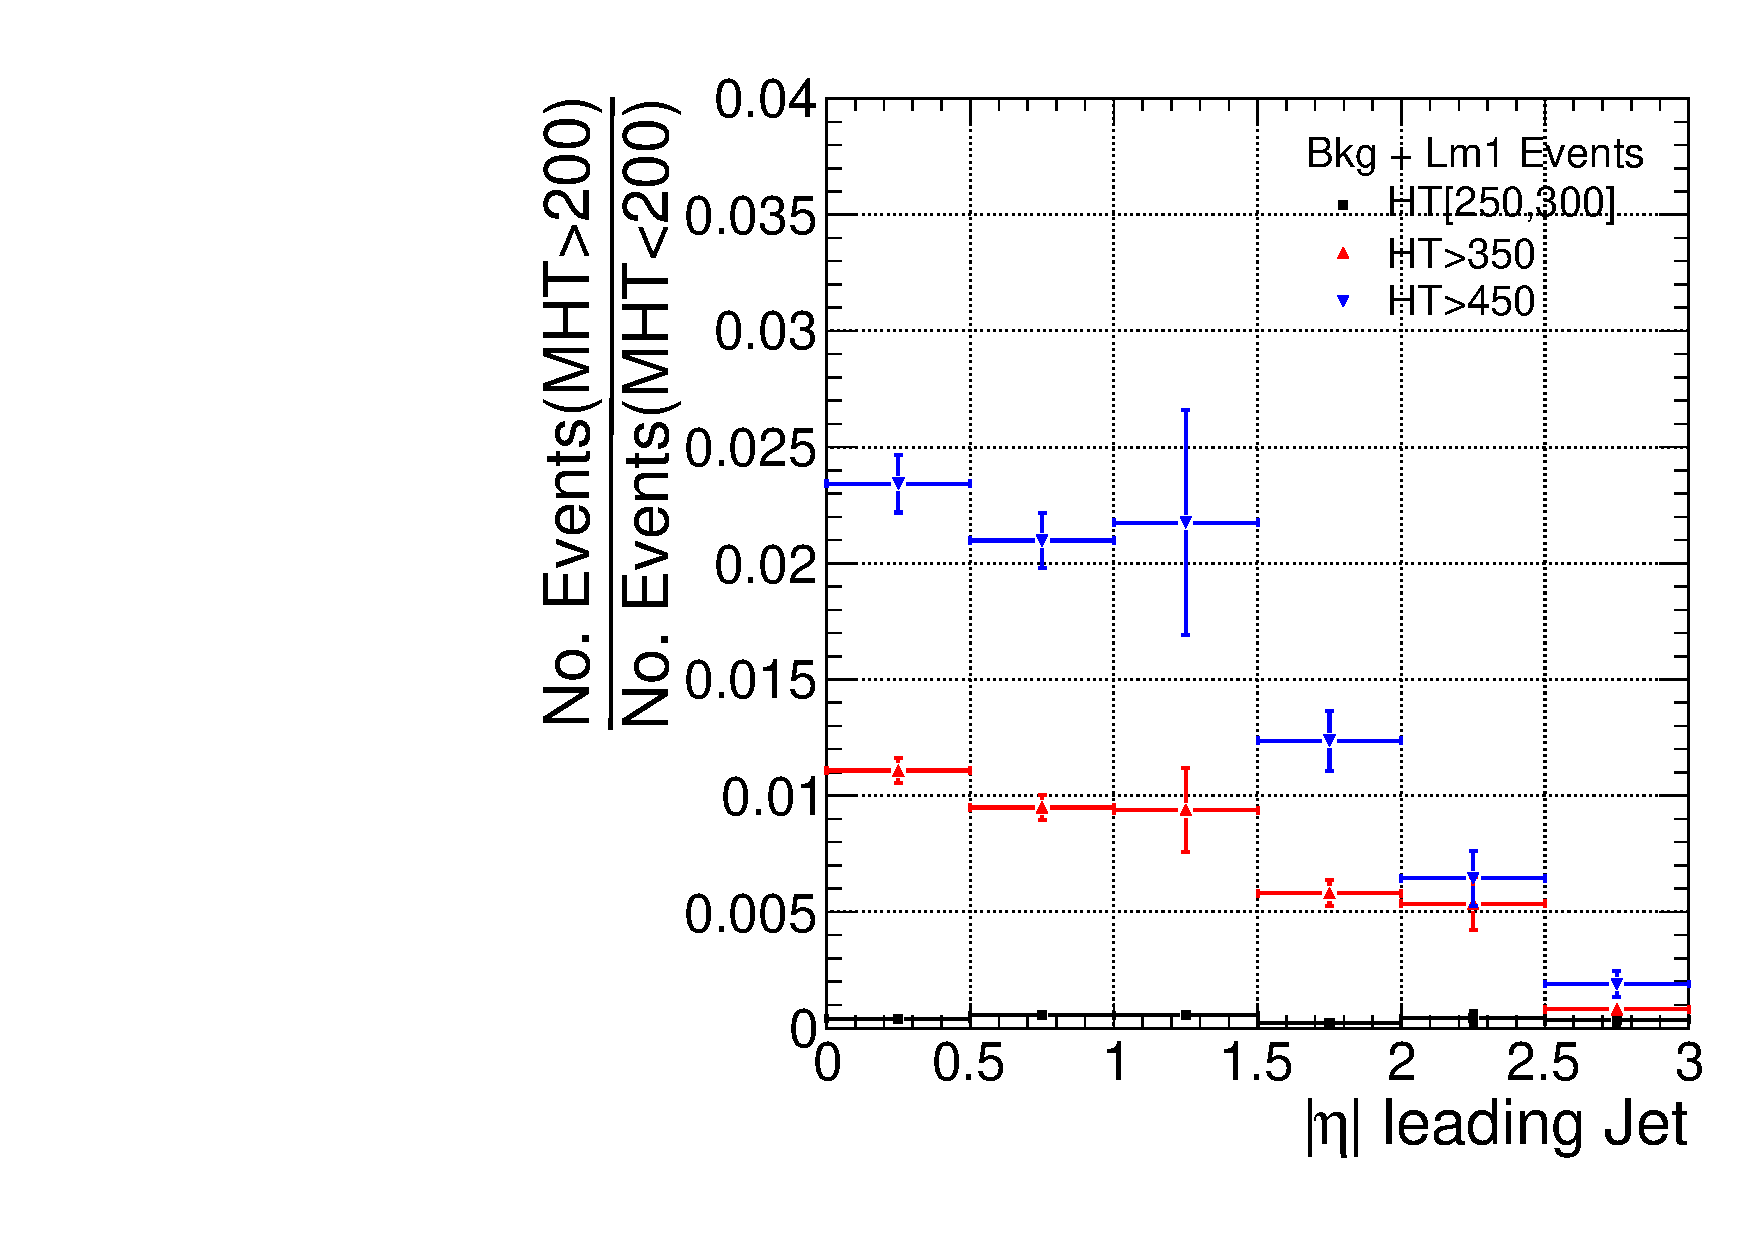
\includegraphics[scale=0.4]{./plots/MHT-NT7-Lm1-MCerr}
\end{minipage}
%  \caption{ }
\label{fig:app4}
\end{figure}

\clearpage
\begin{figure}[h!]
%\begin{minipage}[b]{0.5\linewidth} % A minipage that covers half the page
\centering
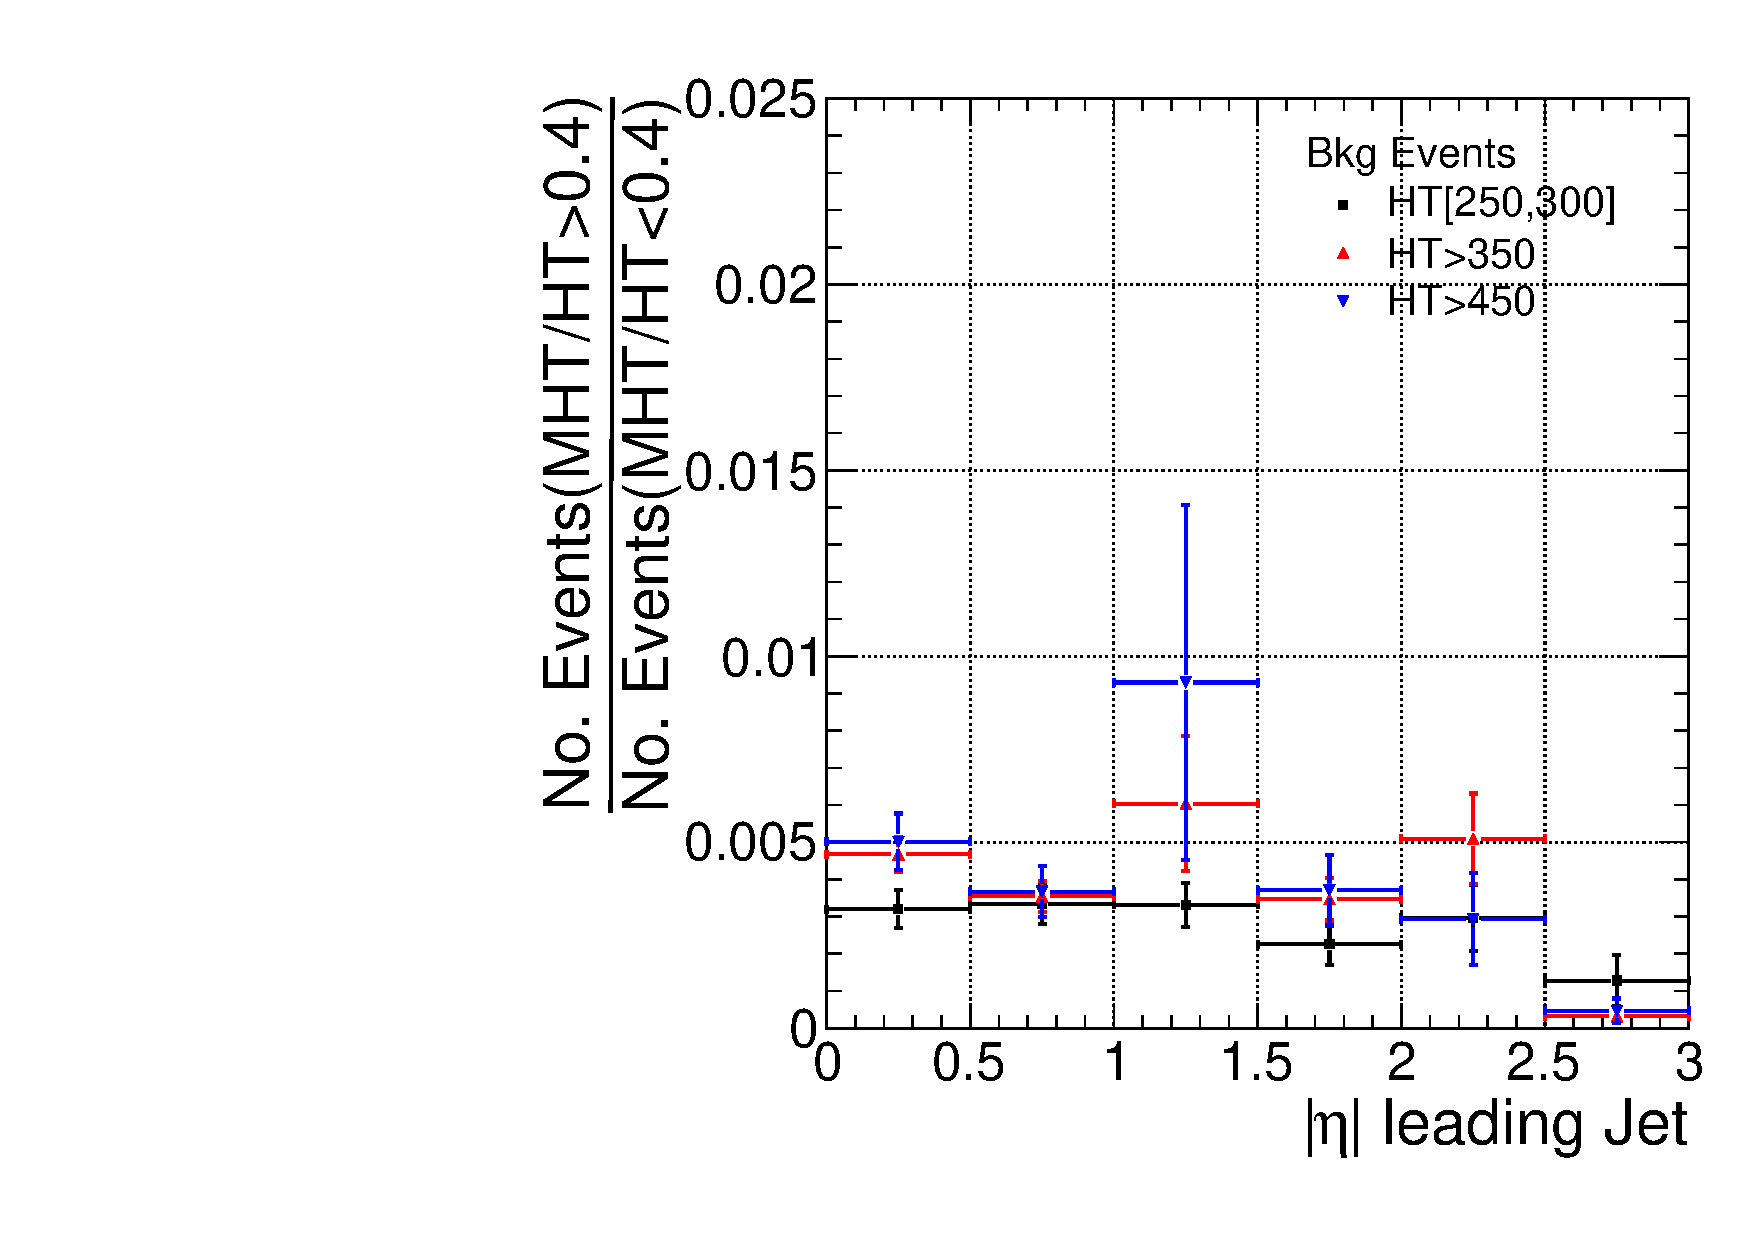
\includegraphics[scale=0.4]{./plots/MHTovHT-NT7-Bkg-MCerr}
%\end{minipage}
%\hspace{0.1cm} % To get a little bit of space between the figures
%\begin{minipage}[b]{0.5\linewidth}
%\centering
%\includegraphics[scale=0.4]{}
%\end{minipage}
%  \caption{ }
\label{fig:id1}
\end{figure}
\begin{figure}[h!]
\begin{minipage}[b]{0.5\linewidth} % A minipage that covers half the page
\centering
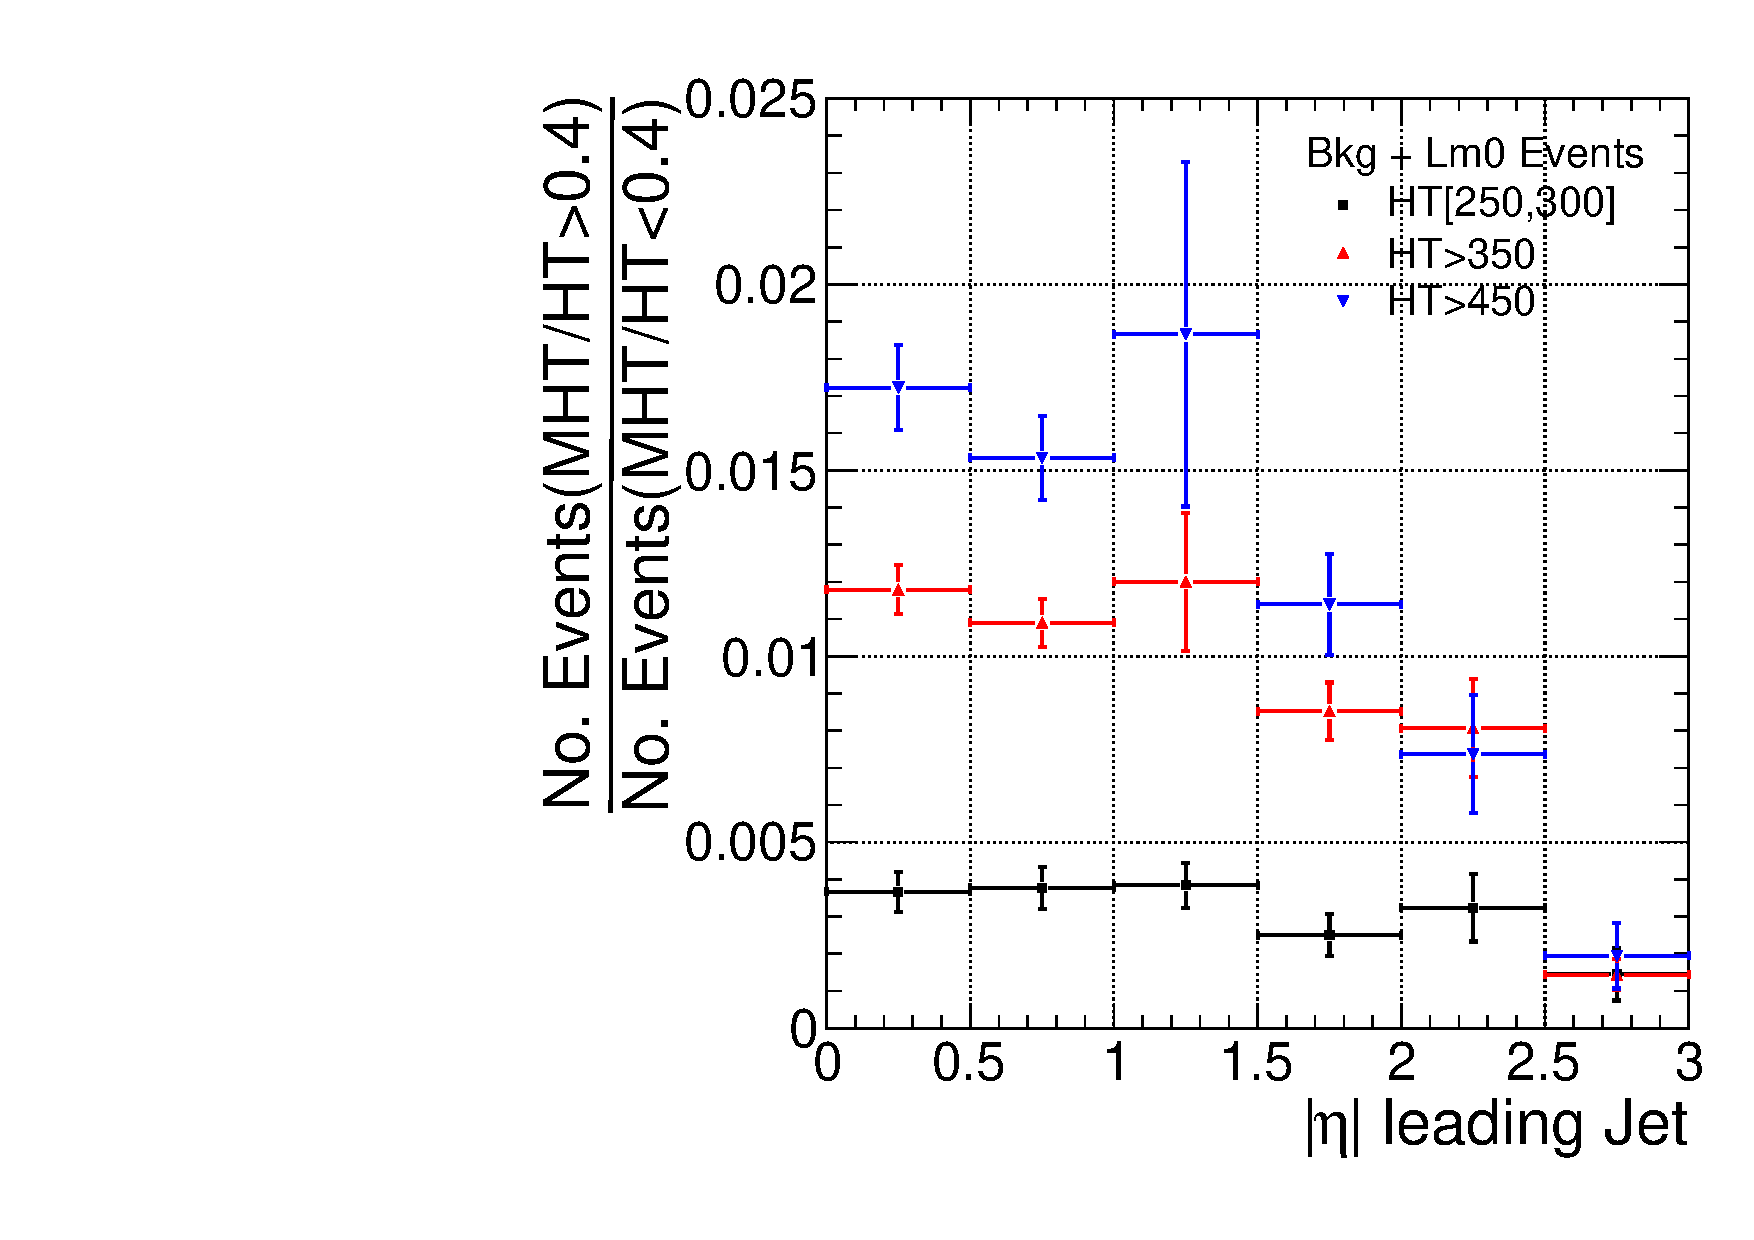
\includegraphics[scale=0.4]{./plots/MHTovHT-NT7-Lm0-MCerr}
\end{minipage}
\hspace{0.1cm} % To get a little bit of space between the figures
\begin{minipage}[b]{0.5\linewidth}
\centering
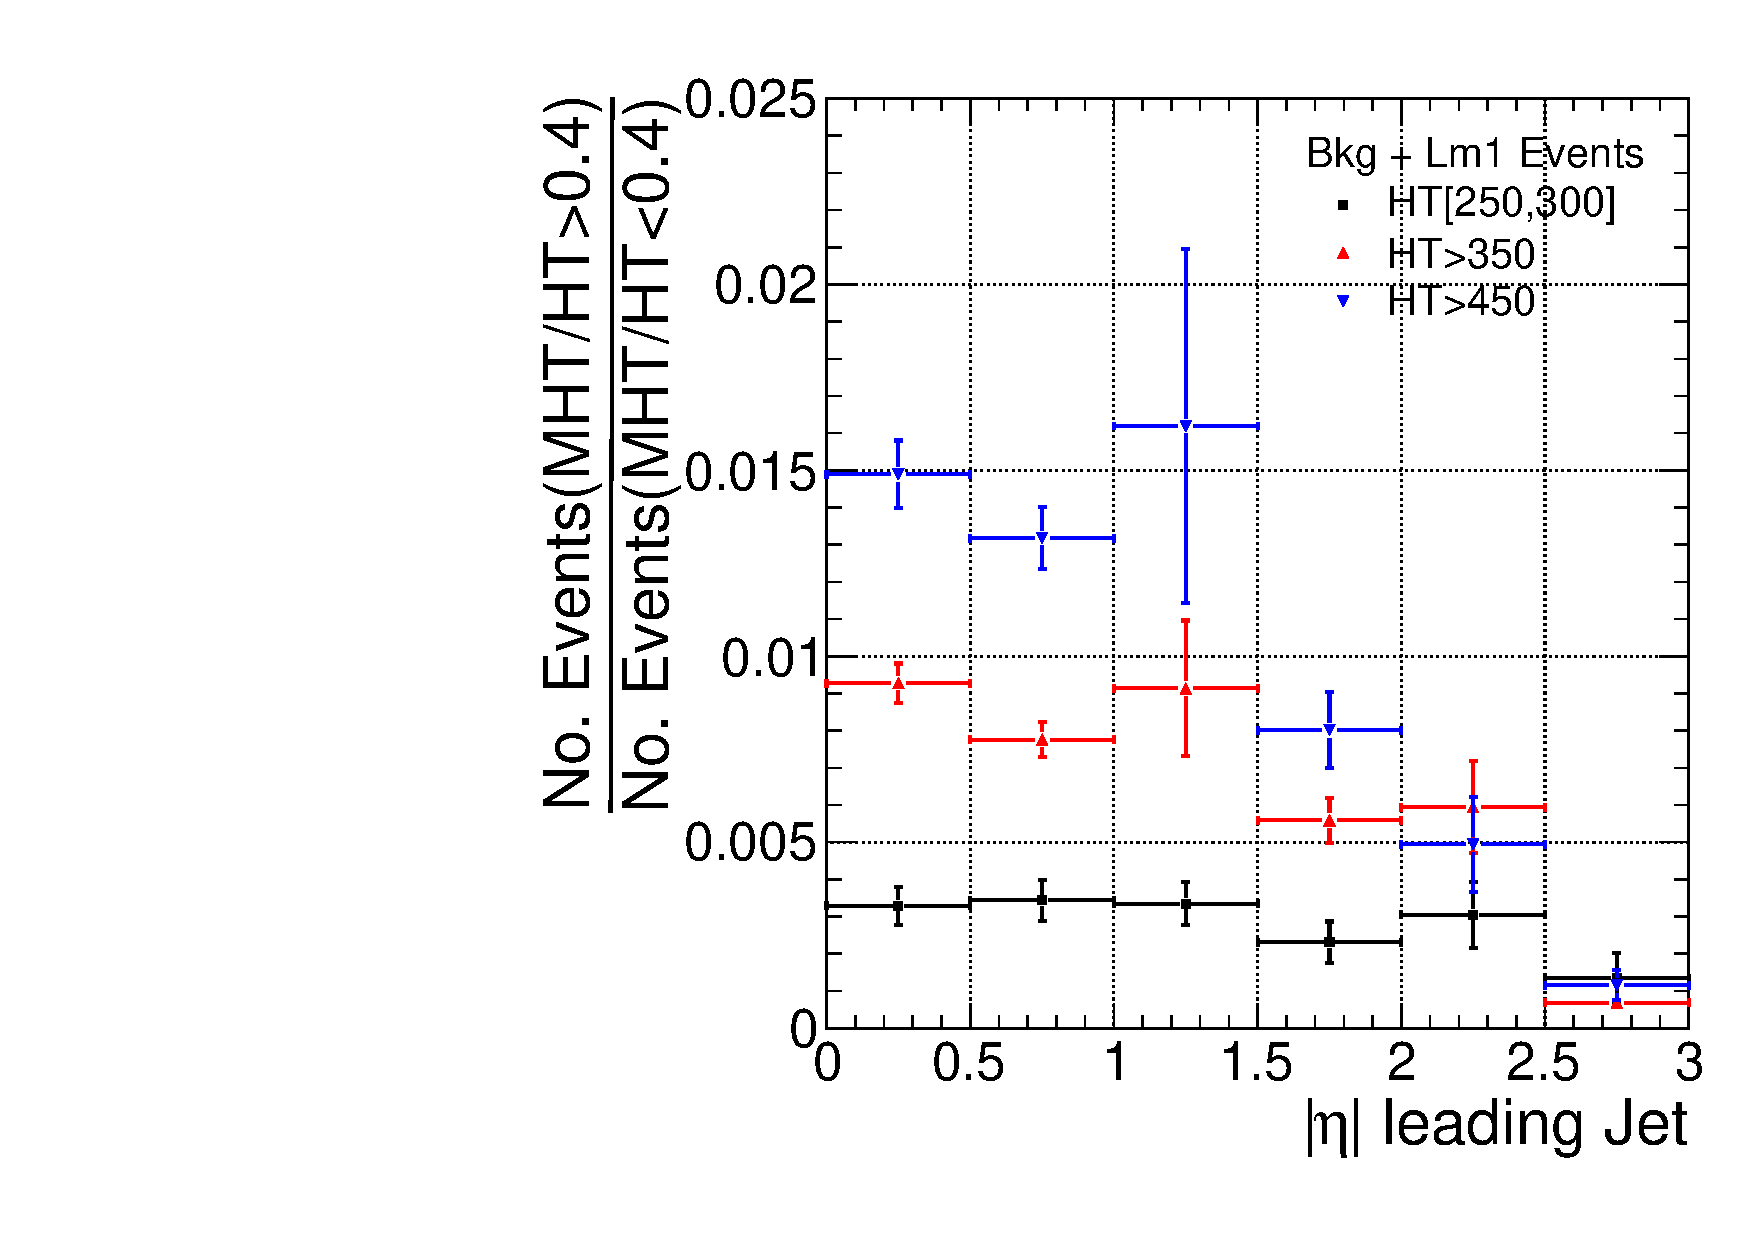
\includegraphics[scale=0.4]{./plots/MHTovHT-NT7-Lm1-MCerr}
\end{minipage}
%  \caption{ }
\label{fig:app5}
\end{figure}
\end{comment}

\clearpage
\section{$M_{eff}$ as an alternative variable choice to $H_{T}$}

$H_{T}$ was chosen for the eta-HT kinematic method as SM processes dominate in the low region, whilst potential SUSY signal can dominate in the higer regions. Another observable which exhibits these characteristics is $M_{eff}$, the sum of $H_{T}$ and $MHT$. We repeat the same analysis as before, using regions of $M_{eff}$ to study $R_{\alpha_{T}}$, having first applied a baseline cut of $H_{T} >$ 350. For this study, we use the same data samples as in the main section, with the exception of the QCD madgraph and $\mathrm{b \bar{b}}$. For these processes we now use a Pythia6 QCD simulation, generated in lower-limit $\hat{p_{T}}$ bins described in Table~\ref{tab:pyth}.As these are inclusive files, care has been taken to remove over-laps. 

\begin{table}[h!]
\centering
\begin{tabular}{|c||c||c|}
\hline
Lower $\hat{p_{T}}$ limit & Number MC Evts & $\sigma$ \\
\hline
\hline
80 GeV & 3477680 & 1934639.6 \\ 
\hline
170 GeV & 3756780 & 62562.9 \\ 
\hline
300 GeV & 1815585 & 3664.6 \\
\hline
470 GeV & 2426752 & 315.5 \\ 
\hline
800 GeV & 2832476 & 11.9 \\ 
\hline
1400 GeV & 584256 & 0.172 \\ 
\hline
2200 GeV & 878796 & 0.00142 \\ 
\hline
3000 GeV & 567040 & 0.0000086 \\
\hline
\end{tabular}
   \caption{\small{\textit{Number of events generated and cross-sections for the Pythia6 QCD Monte Carlo datasets used.They have been generated in inclusive bins with lower limits in $\hat{p_{T}}$. For the study we have taken care to remove all over-laps due to the inclusive binning}}}
 \label{tab:pyth} 
\end{table}

Figure \ref{fig:meff1} displays the distribution of $M_{eff}$ for all the SM backgrounds and the SUSY signal (LM0 and LM1), after the steps of standard selection up to the $\alpha_{T}$ cut. The relationship between SUSY signal and SM background processes clearly changes in the different regions of $M_{eff}$. While background processes clearly dominate for low values, as we increase in $M_{eff}$ they diminish, while signal distributions are still high. Regions of $M_{eff}$ should therefore have largely differing values for $R_{\alpha T}$.


\begin{figure}[h!]
%\begin{minipage}[b]{0.5\linewidth} % A minipage that covers half the page
\centering
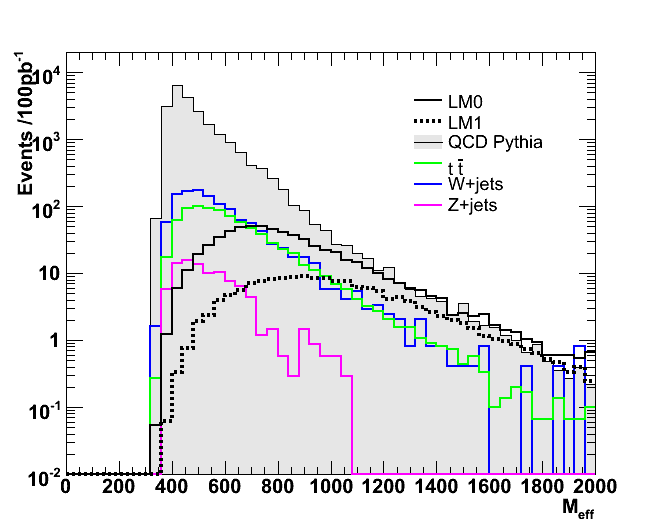
\includegraphics[scale=0.3]{./plots/Meff-NT7-Dist.png}
%\end{minipage}
%\hspace{0.1cm} % To get a little bit of space between the figures
%\begin{minipage}[b]{0.5\linewidth}
%\centering
%\includegraphics[scale=0.4]{}
%\end{minipage}
\caption{\small{\textit{The $M_{eff}$ distribution for the LM0 and LM1 SUSY signal and all the SM backgrounds superimposed, for an intergrated luminosity of 100pb$_{-1}$.}}}
\label{fig:meff1}
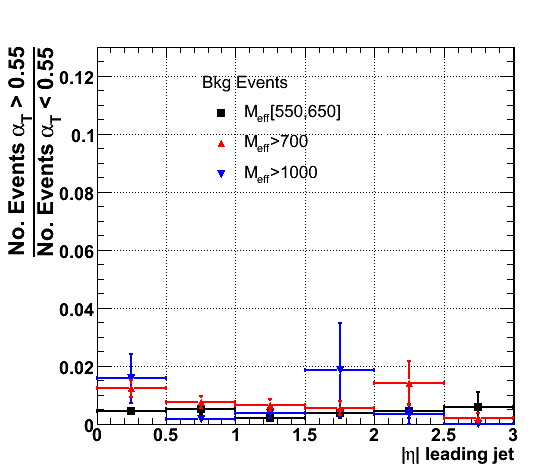
\includegraphics[scale=0.4]{./plots/Meff-NT7-Bkg-MCerr}
%\end{minipage}
%\hspace{0.1cm} % To get a little bit of space between the figures
%\begin{minipage}[b]{0.5\linewidth}
%\centering
%\includegraphics[scale=0.4]{}
%\end{minipage}
\caption{\small{\textit{The $R_{\alpha T}$ versus the leading jet $|\eta|$ for the SM background-only hypothesis, in three $M_{eff}$ bins [550, 650], [700, inf], [1000, inf].} }}
\label{fig:meff2}
\end{figure}

Figure \ref{fig:meff2} shows the $R_{\alpha T}$ versus the $|\eta|$ of the leading jet for the SM background only case, in three chosen regions of $M_{eff}$. The lowest is an exclusive bin with upper and lower limits to choose control region only, and in addition two inclusive bins with lower limits only. The distribution of $R_{\alpha T}$ in this background-only hypothesis is flattish for all regions, as in the $H_{T}$ case. This is expected as for background processes the leading jet has little predisposition to centrality. 
In figures \ref{fig:meff3}, we plot the value of $R_{\alpha T}$ for the SUSY signal LM0 (left) and LM1 (right) respectively, plus the SM background, versus $|\eta|$ of the leading jet. Comparing these to the background-only hypothesis, it can be seen a significant deviation occurs, increasing in Meff bins. The signal case is more central than the background-only, and this is more pronounced as we move to higher regions of $M_{eff}$, where the signal is more prominent against background. 

Comparing these to the $H_{T}$ case, we see the same characteristics. Numerically the gain in $R_{\alpha T}$ is on a greater scale than that seen in the $H_{T}$ case, but the errors are larger too. In order to inspect the deviation quantitatively, the $R_{\alpha T}$ distribution is fitted, as previously done for HT. The $R_{\alpha T}$ vs the $|\eta|$ of ther leading jet is fitted with a 1st degree polynomial ($p0+p1.|\eta|$) using the $\chi^{2}$ method. The corresponding plots of the parameters of the fit are seen in Figure~\ref{fig:meff4} for the cases with and without signal. As in the HT case, the background-only picture shows flat distribution in $M_{eff}$ for both p0 and p1, while the SUSY signal is much more pronounced in regions of high $M_{eff}$ than in the low control region. It can also be seen that for LM0, the deviation from the background picture reaches a plateau at 750 GeV while for LM1 it continues. This is inherent from the mass spectrum of the LM0 case. 
\begin{figure}[h!]
\begin{minipage}[b]{0.5\linewidth}
\centering
{\label{fig:lm0_RaT}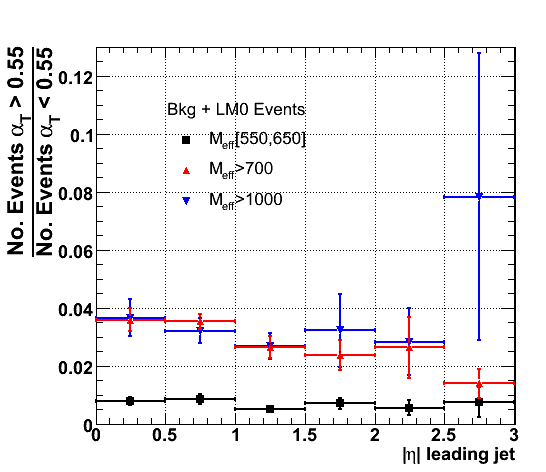
\includegraphics[scale=0.4]{./plots/Meff-NT7-Lm0-MCerr}} 
\end{minipage}
\begin{minipage}[b]{0.5\linewidth}
\centering
{\label{fig:lm1_RaT}\includegraphics[scale=0.4]{./plots/Meff-NT7-Lm1-MCerr}} 
\end{minipage}
\caption{\small{\textit{The $R_{\alpha T}$ versus the leading jet $|\eta|$ for the SUSY signal (LM0 on the left, LM1 on the right) plus SM background hypothesis, in three $M_{eff}$ bins [550, 650], [700, inf], [1000, inf].} }}
\label{fig:meff3}
\end{figure}


\begin{figure}[h!]
\begin{minipage}[b]{0.5\linewidth}
\centering
{\label{fig:meff_p0}\includegraphics[scale=0.4]{./plots/Meff-NT7-p0-MCerr}} 
\end{minipage}
\begin{minipage}[b]{0.5\linewidth}
\centering
{\label{fig:meff_p1}\includegraphics[scale=0.4]{./plots/Meff-NT7-p1-MCerr}} 
\end{minipage}
\caption{\small{\textit{The parameters p0(left) and p1(right) of the first-degree polynomial fit to the $R_{\alpha T}$ versus $|\eta|$ curves, for each value of lower $M_{eff}$ limit [GeV]. Each plot shows three scenarios: background-only hypothesis, and background with added LM0/LM1 signal.}}}
\label{fig:meff4}
\end{figure}


In order to compare the use of $M_{eff}$ in this method to that of HT, we again calculate the quantity $\Delta p_{i} / \sigma$, to consider the significance of the difference between the parameters with and without LM1 signal. Figures~\ref{fig:meff5} and \ref{fig:meff6} show the intercept and gradient plots for Meff (left) against the same plots for HT (right) for comparison. It can be seen that the significance of the intercept increases faster for $M_{eff}$ than for HT, but the corresponding plots for the gradient indicate that using $M_{eff}$ in this method produces less stable results. 

From these plots we can conclude that increasing lower limits in $M_{eff}$ allow a change from a region where SM processes dominate to where SUSY signal is prolific. Thus this variable can be used instead of HT along with $|\eta|$ to establish a deviation from the Standard Model. The deviation apears more pronounced than for the HT method, but significance plots show a more erratic behaviour. Until this behaviour is understood, and can be controlled, more reliable results will be seen with the HT method. 




 




\begin{figure}[h!]
\begin{minipage}[b]{0.5\linewidth}
\centering
{\label{fig:meff_p0_s}\includegraphics[scale=0.4]{./plots/Meff-NT7-p0-Sig}} 
\end{minipage}
\begin{minipage}[b]{0.5\linewidth}
\centering
{\label{fig:HT_p0_s}\includegraphics[scale=0.4]{./plots/HT-NT7-p0-Sig}} 
\end{minipage}
\caption{\small{\textit{ $\Delta p_{i} / \sigma$ of the parameter p0 of the fit to the $R_{\alpha T}$ vs. $|\eta|$ plots for $M_{eff}$ (left) and $H_{T}$ (right). This is a measure of 'significance' for establishing a SUSY deviation to the SM-only hypothesis using this parameter.}}}
\label{fig:meff5}
\end{figure}



\begin{figure}[h!]
\begin{minipage}[b]{0.5\linewidth}
\centering
{\label{fig:meff_p1_s}\includegraphics[scale=0.4]{./plots/Meff-NT7-p1-Sig}} 
\end{minipage}
\begin{minipage}[b]{0.5\linewidth}
\centering
{\label{fig:HT_p1_s}\includegraphics[scale=0.4]{./plots/HT-NT7-p1-Sig}} 
\end{minipage}
\caption{\small{\textit{ $\Delta p_{i} / \sigma$ of the parameter p1 of the fit to the $R_{\alpha T}$ vs. $|\eta|$ plots for $M_{eff}$ (left) and $H_{T}$ (right). This is a measure of 'significance' for establishing a SUSY deviation to the SM-only hypothesis using this parameter.} }}
\label{fig:meff6}
\end{figure}

\end{document}
